\documentclass{article}
\usepackage[utf8]{inputenc}
\usepackage{hyperref}
\usepackage{natbib}
\usepackage{times}
\usepackage{amsfonts}
\usepackage{amsmath}
\usepackage{amssymb}
\usepackage{amstext}
\usepackage{amsthm}
\usepackage{bbm}
\usepackage{latexsym}
\usepackage{color}
\usepackage{graphicx}
\usepackage{subfigure}
\usepackage{enumerate}
\usepackage{float}
\usepackage{caption}
\captionsetup[figure]{font=small}
\usepackage[justification=centering]{caption}
\usepackage{algorithm}
\usepackage[noend]{algpseudocode}
\usepackage{fullpage}
\usepackage{array}
\newtheorem{theorem}{Theorem}
\newtheorem{lemma}[theorem]{Lemma}

\title{SURE report}
\author{Xinyu Li, Ziyu Lu}
\date{August 2019}

\begin{document}

\maketitle

\section{Introduction} 
Stochastic optimization is an old subject given new life by application to machine learning. Among the numerous variants of the classical gradient descent algorithm, the Adagrad algorithm\cite{duchi2011adaptive}, the Adam algorithm\cite{kingma2014adam}, and the RMSprop algorithm\cite{tieleman2012lecture} are particularly well-known. They have been proven to be more effective than the vanilla gradient descent algorithm especially with deep neural networks, where the optimization problem is usually nonlinear and high-dimensional. While these algorithms have been widely applied in machine learning, little effort has been made to adapt them to stochastic optimal control problems beyond this field. The aim of our project, therefore, is to apply these innovative stochastic optimization algorithms to stochastic optimal control problems which are traditionally thought to be outside their specialty. In most stochastic optimal control problems, the actual control is impossible to calculate. As a matter of fact, the control can only be computed in exact formulas when it is designed to be linear quadratic and the problem is low dimensional. As real world problems are usually more complicated with nonlinear control and high dimensionality, the actual control cannot be calculated. In this report, we propose that we can first parameterize the control and then employ stochastic optimization algorithms from machine learning to estimate its parameters.

\bigskip
\noindent The report is organized as follows: In section 2, we solve a linear quadratic gaussian problem with Kalman filter and linear control, where the theoretical optimal control is avaliable. We compare the results given by machine learning optimization algorithms with the theoretical solution, and conduct a series of experiments to tune the parameters in the algorithms. In section 3, we move on to the nonlinear insulin control problem, where theoretical solution no longer exists and we rely on the machine learning optimization algorithms to obtain the control. In section 4, we close the report with a discussion on our results and a reflection on this project.

\section{Linear quadratic gaussian control problem}
\subsection{Model}
Consider a spring-mass model described by the 2D Ornstein-Uhlenbeck process:
\[
\begin{cases}
	dx = vdt \\ dv = (-\frac{k}{m}x - \frac{\gamma}{m}v)dt + \sigma dW 
\end{cases}
\]
%\begin{equation*}
%\begin{pmatrix}dx\\dv\end{pmatrix}= \begin{pmatrix}0 & 1 \\ -\frac{k}{m}  & -\frac{\gamma}{m}\end{pmatrix}\begin{pmatrix}x\\v\end{pmatrix} dt+ \begin{pmatrix}0 & 0 \\0 &\sigma\end{pmatrix}\begin{pmatrix}dW_t^{(1)}\\dW_t^{(2)}\end{pmatrix}
%\end{equation*}
where $x$, $v$ are the position and the velocity of the object, $k$ is the spring constant, $\gamma$ is the friction coefficient, $\sigma$ is the noise coefficient, and $W$ is a Wiener process. \\
To prepare for the insulin control problem where the observation is discrete, we discretize the state and observation of the system into a series of time steps: Let $T = N\Delta t$, $X_n = \begin{pmatrix}x(n\Delta t)\\v(n\Delta t)\end{pmatrix}, \ n = 0,1,\dots, N$. Then by spectral decomposition, the dynamics of the system can be captured by
\begin{equation*}
X_{n+1} = AX_n + W_n
\end{equation*}
where 
\begin{equation*}
A = A(\Delta t) = \frac{1}{\lambda_{2}-\lambda_{1}}\left(\begin{array}{ll}{\lambda_{2} e^{\lambda_{1} \Delta t}-\lambda_{1} e^{\lambda_{2} \Delta t}} & {-e^{\lambda_{1} \Delta t}+e^{\lambda_{2} \Delta t}} \\ {\lambda_{1} \lambda_{2}\left(e^{\lambda_{1} \Delta t}-e^{\lambda_{2} \Delta t}\right)} & {-\lambda_{1} e^{\lambda_{1} \Delta t}+\lambda_{2} e^{\lambda_{2} \Delta t}}\end{array}\right) 
\end{equation*}
and $\lambda_1 = -\frac{\gamma}{2m} + i\sqrt{\frac{4km-\gamma^2}{4m^2}}$, $\lambda_2 = -\frac{\gamma}{2m} - i\sqrt{\frac{4km-\gamma^2}{4m^2}}$. 
$W_n$ is a gaussian noise with mean 0 and covariance $R$, where 
\begin{equation*}
R = \left(\frac{\sigma}{\lambda_{2}-\lambda_{1}}\right)^{2}
    \begin{pmatrix}
    \frac{e^{2 \lambda_{1} \Delta t}-1}{2 \lambda_{1}}+\frac{e^{2 \lambda_{2} \Delta t}-1}{2 \lambda_{2}}-2 \frac{e^{\left(\lambda_{1}+\lambda_{2}\right) \Delta t}-1}{\left(\lambda_{1}+\lambda_{2}\right)} 
    & \frac{e^{2 \lambda_{1} \Delta t}-1}{2 }+\frac{e^{2 \lambda_{2} \Delta t}-1}{2 }- ({e^{\left(\lambda_{1}+\lambda_{2}\right) \Delta t}-1})  \\
    \frac{e^{2 \lambda_{1} \Delta t}-1}{2 }+\frac{e^{2 \lambda_{2} \Delta t}-1}{2 }- ({e^{\left(\lambda_{1}+\lambda_{2}\right) \Delta t}-1})  & 
     \lambda_{1}\frac{e^{2 \lambda_{1} \Delta t}-1}{2}+\lambda_{2}\frac{e^{2 \lambda_{2} \Delta t}-1}{2 }-2 \lambda_{1}\lambda_{2}\frac{e^{\left(\lambda_{1}+\lambda_{2}\right) \Delta t}-1}{\left(\lambda_{1}+\lambda_{2}\right)} \end{pmatrix}
\end{equation*}
With control, the state update becomes
\begin{equation*}
    X_{n+1} = AX_n + BU_n + W_n
\end{equation*}
where $U_n$ denotes the control at time step $n$, and $B = \begin{pmatrix} 0 \\1 \end{pmatrix}$.\\
The observation can be expressed as 
\begin{equation*}
Z_{n+1} = CX_{n+1} + V_{n+1}
\end{equation*}
where $C = \begin{pmatrix} 1 & 0\end{pmatrix}$, and $V_n$ is a gaussian noise with mean 0 and covariance $S$, $V_n$ independent of $W_n\ \forall n$.\\
Using a Kalman filter, the state estimation update is given by
\begin{equation*}\label{eq:est}
\widehat{X}_{n+1} = A\widehat{X}_n + BU_n + K(Z_{n+1} - C(A\widehat{X}_n + BU_n))
\end{equation*}
where $K$ denotes the Kalman gain, and $\widehat{X}_0 \equiv X_0$.\\
Define cost rate
\begin{equation*}
    J_n(G) = \mathbb{E}[ |X_{n+1}|^2+r|U_{n}|^2 ], \quad \text{for } n = 0, 1, \dots, N-1
\end{equation*}
and the total cost
\begin{equation*}
F(K,G) = \frac{1}{2N} \mathbb{E} [ \sum_{n=0}^{N-1} (X_{n+1}^T X_{n+1} + r U_n^T U_n)]
\end{equation*}
Our goal is to find the optimal $K$ and $G$ such that the cost $F(K,G)$ is minimized.
\subsection{Theoretical solution}
\subsection{Optimization with machine learning optimization algorithms}
\subsubsection{Review of RMSprop algorithm}
The RMSprop algorithm is an adaptive learning rate method proposed by Geoff Hinton in Lecture 6e of his Coursera Class \cite{tieleman2012lecture}. The basic idea of RMSprop algorithm is summarized in algorithm \ref{alg:rmsprop}.
\begin{algorithm}
	\caption{RMSprop}
	\begin{algorithmic}
		\State \textbf{Input:} Cost function $f$, total number of gradient descent iterations $n$, learning rate $\alpha$, smoothing constant $\beta$, initial value of the parameter(s) to be optimized $\theta_0$, initial $\phi_0 = 0$, term added to denominator to avoid divide-by-zero error $\epsilon$.
		\For{$i = 1,2,\dots, n$}
		\State Compute the cost with the parameter(s) at the current iteration $f(\theta_i)$
		\State Compute the gradient $g_i = \frac{\partial f(\theta_i)}{\partial \theta_i}$
		\State Update $\phi_i$: $\phi_i = \beta \phi_{i-1} + (1-\beta) g^2_i$ (element-wise square)
		\State Update $\theta_i$: $\theta_i = \theta_{i-1} - \alpha\frac{g_i}{\sqrt{\phi_i + \epsilon}}$
		\EndFor
	\end{algorithmic}
	\label{alg:rmsprop}
\end{algorithm}

\subsubsection{Gradient calculation}
At each iteration, the gradient $g_i$ is calculated using a backward recurrence relation:\\
Assume $\widehat{X}_0 = X_0 = x_0$. Define the total cost
\[
F(K,G) = \sum_{n=0}^{N-1} (X_n^T X_n + r U_n^T U_n) + X_N^T X_N
\]
In practice, we store the value of $U_N$ as 0, so we can simply compute $F(K,G) = \sum_{n=0}^{N} (X_n^T X_n + rU_n^2)$. This is a random variable that depends on $K$, $G$ and the random noise $W_n$ and $V_n$.
For $K$ and $G$ fixed, the expectation is 
\[
V_0(x_0,x_0,K,G) \triangleq \text{E}\left[F \right]
\]
The random cost starting at time $j$ with $\widehat{X}_j = \widehat{x}$, $X_j = x$ is
\[
F_j(x, \widehat{x},K,G, V_{[j+1,\ldots,N]},X_{[j+1,\ldots,N]}) = \sum_{n=j}^N (X_n^T X_n + rU_n^T U_n)
\]
In this formula, $\widehat{X}_j = \widehat{x}$, $X_j = x$, so the $n=j$ term is $x^T x + rU_j^2$.
Assume the ``initial'' condition at time $n=j$ is given by $x$ and $\widehat{x}$, then the cost-to-go function is 
\[
V_j(x,\widehat{x},K,G) = \text{E} \!\left[\, F_j(x,\widehat{x},K,G\ldots)\right] \; .
\]
The optimal filtering and control problem, therefore, is to choose $K$ and $G$ to minimize $V_0(x_0,x_0,K,G)$, and we need to compute $\nabla_K V_0(x_0,x_0,K,G)$ and $\nabla_G V_0(x_0,x_0,K,G)$.

\noindent Define 
\[
Q_j \triangleq \nabla_K F_j(x, \widehat{x},K,G\ldots), \quad H_j \triangleq \nabla_G F_j(x, \widehat{x},K,G\ldots)
\]
then 
\[
\nabla_K V_j(x,\widehat{x},K,G) = \mathbb{E}[Q_j], \quad \nabla_G V_j(x,\widehat{x},K,G) = \mathbb{E}[H_j]
\]

\noindent Other important quantities are the gradients of the random cost and the cost-to-go functions with respect
to $x$ and $\widehat{x}$.
Define
\[
P_j(x,\widehat{x},K,G\ldots) \triangleq \nabla_{\widehat{x}} F_j(x,\widehat{x},K,G\ldots)
\]
\[
T_j(x,\widehat{x},K,G\ldots) \triangleq \nabla_{x} F_j(x,\widehat{x},K,G\ldots)
\]
then
\[
\nabla_{\widehat{x}} V_j(x, \widehat{x},K,G\ldots) 
= \text{E} \!\left[\, P_j(x,\widehat{x},K,G\ldots)\right]
\]
\[
\nabla_{x} V_j(x, \widehat{x},K,G\ldots) 
= \text{E} \!\left[\, R_j(x,\widehat{x},K,G\ldots)\right]
\]
An algorithm for computing $Q_j$, $H_j$ uses $P_j$ and $T_j$.
The $P_j$ and $T_j$ are computed using a backward recurrence.

\noindent Start with 
\[
F_N = X_N^T X_N + rU_N^T U_N
\]
The derivative with respect to $K$ is zero, and the derivative with respect to $G$ is 0 (since $U_N = 0$).
The derivative with respect to $\widehat{x}$ (in numerator-layout) is
\[
P_N =  2rU_N^T\frac{\partial U_N}{\partial \widehat{x}_N} = 2rU_N^TG = 0
\]
The derivative with respect to $x$ (in numerator-layout) is
\begin{align*}
T_N &= 2X^T_N + 2rU_N^T\frac{\partial U_N}{\partial \widehat{x}_N}\frac{\partial \widehat{x}_N}{\partial x_N} \\
&= 2X^T_N + 2rU_N^TGKC = 2X^T_N
\end{align*}
From this start, the rest of the derivatives are calculated using back-propagation.
The backward recurrence relation is
\[
F_j(x,\widehat{x},K,G\ldots) = x^T x + rU_j^2 + F_{j+1}(X_{j+1},\widehat{X}_{j+1}, K,G\ldots)
\]
In this formula, $X_{j+1}$ is a function of $x$, $\widehat{x}$, $G$, and $\widehat{X}_{j+1}$ is a function of $x$, $\widehat{x}$, $K$ and $G$.
\begin{align*}
X_{j+1} = Ax + BG\widehat{x} + W_j
\end{align*}
\begin{align*}
\widehat{X}_{j+1} &=  (A+BG) \widehat{x}  + K(Z_{j+1} - C(A+BG)\widehat{x}) \\
& = (I-KC)(A+BG) \widehat{x} + KZ_{j+1} \\
&= (I-KC)(A+BG) \widehat{x} + K(CX_{j+1} + V_{j+1}) \\
&= (I-KC)(A+BG)\widehat{x}+K(CAx+CBG\widehat{x}+CW_j+V_{j+1})\\
&= [(I-KC)A+BG]\widehat{x}+KCAx+KCW_j+KV_{j+1} 
\end{align*}
The recurrence relations for $P_j$ and $T_j$ use the chain rule and differentiates the above update formulas for $X$ and $\widehat{X}$ 
\[
\nabla_{\widehat{x}} X_{j+1} = BG, \quad \nabla_{x} X_{j+1} = A
\]
\[
\nabla_{\widehat{x}} \widehat{X}_{j+1} = [(I-KC)A + BG], \quad \nabla_{x} X_{j+1} = KCA
\]
The chain rule gives (in numerator-layout)
\begin{align*}
P_j = \nabla_{\widehat{x}} F_j 
&= \nabla_{\widehat{x}}(x^Tx + rU_j^TU_j)
+ \nabla_{\widehat{x}}F_{j+1}(X_{j+1},\widehat{X}_{j+1},K,G \ldots) \\
&= 2rU_j^TG + \nabla_{\widehat{X}_{j+1}}F_{j+1} \nabla_{\widehat{x}} \widehat{X}_{j+1}+ \nabla_{X_{j+1}}F_{j+1} \nabla_{\widehat{x}} X_{j+1}\\
&= 2rU_j^TG 
+ P_{j+1}[(I-KC)A + BG] + T_{j+1}BG
\end{align*}
\begin{align*}
T_j = \nabla_{x} F_j &= \nabla_{x}(x^Tx + rU_j^TU_j) + \nabla_{x}F_{j+1}(X_{j+1},\widehat{X}_{j+1},K,G \ldots) \\
&= 2x^T  + \nabla_{X_{j+1}}F_{j+1} \nabla_{x} X_{j+1} + \nabla_{\widehat{X}_{j+1}}F_{j+1} \nabla_{x} \widehat{X}_{j+1} \\
&= 2x^T  + T_{j+1}A + P_{j+1}KCA 
\end{align*}

\noindent Since 
\[
\widehat{X}_{n+1} = A \widehat{X}_n+BU_n+K(Z_{n+1}-C(A\widehat{X}_n+BU_n))
\]
we have 
\[
\nabla_K \widehat{X}_{j+1} = \text{diag}\{(Z_{j+1}- C(A\widehat{x}+BU_j))\}
\]
\[
\nabla_G\widehat{X}_{j+1} = (I-KC)B\widehat{x}^T
\]
so
\begin{align*}
Q_j 
&= \nabla_K (x^Tx + rU_j^TU_j) 
+ \nabla_K F_{j+1}
+ \nabla_{\widehat{X}_{j+1}} F_{j+1} \nabla_K \widehat{X}_{j+1} + \nabla_{X_{j+1}} F_{j+1} \nabla_K X_{j+1} \\
&= Q_{j+1} + P_{j+1}\cdot \text{diag}\{(Z_{j+1}- C(A\widehat{x}+BU_j))\}
\end{align*}
Since
\[
X_{n+1}=AX_n+BU_n+W_n
\]
we have 
\[
\nabla_G X_{j+1} = B\widehat{x}^T
\]
So
\begin{align*}
H_j &= \nabla_G (x^Tx + rU_j^TU_j) 
+ \nabla_G F_{j+1}
+ \nabla_{\widehat{X}_{j+1}} F_{j+1} \nabla_G\widehat{X}_{j+1} + \nabla_{X_{j+1}} F_{j+1} \nabla_G X_{j+1} \\
&= 2rU_j^T\widehat{x}^T + H_{j+1} + P_{j+1}(I-KC)B\widehat{x}^T + T_{j+1} B\widehat{x}^T
\end{align*}

\subsubsection{Hyper-parameter settings}
According our experiments, the hyper-parameters that have dominant influence on the performance of the algorithm are: total number of gradient descent iterations $n$, smoothing constant $\beta$, and mini-batch size $M$. To investigate the impacts of these three factors, we fix other hyper-parameters as constants and list them here.
\begin{itemize}
	\item mass of the object $m = 1$
	\item spring constant $k = 1$
	\item friction coefficient $\gamma = 0.1$
	\item noise coefficient in SDE $\sigma = 0.1$
	\item covariance of observation noise $S = 0.3$
	\item initial displacement $x_0 = 1$
	\item initial velocity $v_0 = 0$
	\item initial state $X_0 = [x_0, v_0]^T = [1.0, 0.0]^T$
	\item total time in one simulation $t_1 = 30$
	\item step size in one simulation $dt = 1.5$
	\item total time steps in one simulation $N = \frac{t_1}{dt} + 1 = 21$
	%\item algorithm: RMSprop
	\item learning rate $\alpha = 0.1$
	%\item smoothing constant $\beta = 0.99$ (default value in PyTorch)
	%\item mini-batch size $M = 8$
	%\item number of gradient descent iterations $n = 2000$
	\item initial Kalman gain $K_0 = [0.5, 0.5]^T$
	\item initial control gain $G_0 = [-1.0, -0.1]$
	\item random seed $s = 1$
\end{itemize}

\subsubsection{Theoretical result}
In the steady state, $K = [1.12\times 10^{-1},  2.44\times 10^{-3}]^T$,
$G = [6.49\times 10^{-1}, -4.89\times 10^{-2}]$. The cost simulating with $K$, $G$ in the steady state is $5.37\times 10^{-2}$.\\
Evolution of displacement $x$, velocity $v$, Kalman gain $K$, and control gain $G$ w.r.t. time are plotted in figures \ref{fig:x_t} to \ref{fig:G_t}.\\

\begin{figure}[h!]
	\centering
	\begin{minipage}[t]{.27\paperwidth}
		\centering
		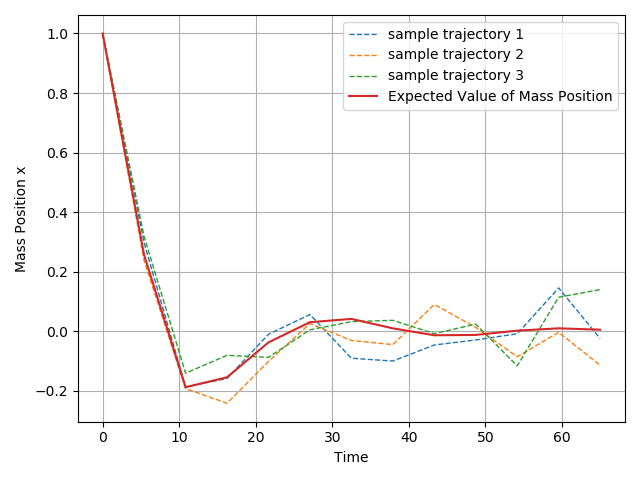
\includegraphics[width=1.0\textwidth]{Figures/x_t.png}
		\caption{$x$ w.r.t $t$: sample trajectories and \\ expected value \label{fig:x_t}}
	\end{minipage}%
	\begin{minipage}[t]{.27\paperwidth}
		\centering
		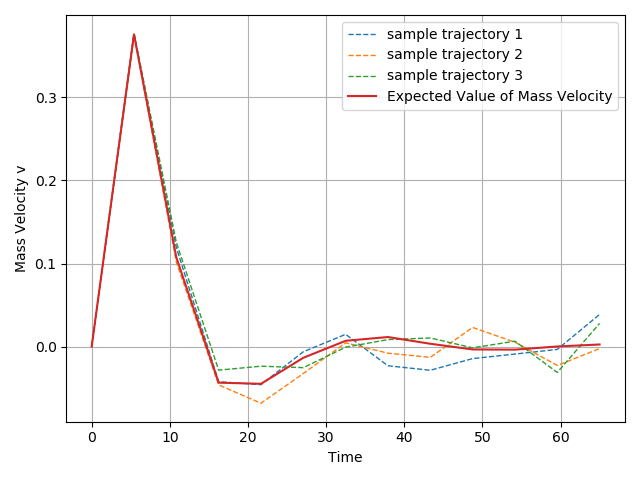
\includegraphics[width=1.0\textwidth]{Figures/v_t.png}
		\caption{$v$ w.r.t $t$: sample trajectories and \\ expected value \label{fig:v_t}}
	\end{minipage}
\end{figure}

\begin{figure}[h!]
	\centering
	\begin{minipage}[t]{.27\paperwidth}
		\centering
		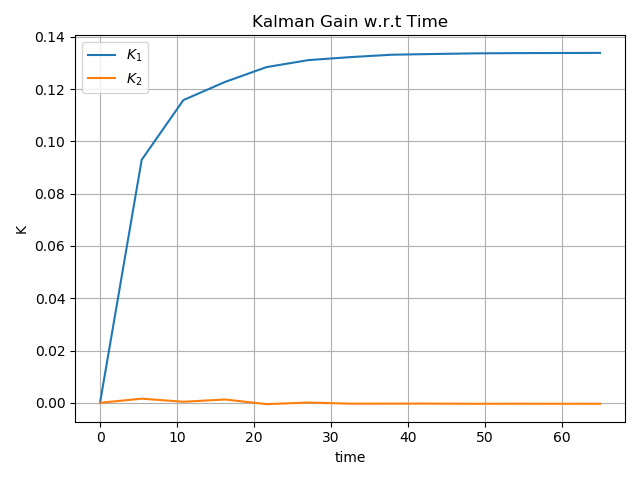
\includegraphics[width=1.0\textwidth]{Figures/K_t.png}
		\caption{Kalman gain $K$ w.r.t time\label{fig:K_t}}
	\end{minipage}%
	\begin{minipage}[t]{.27\paperwidth}
		\centering
		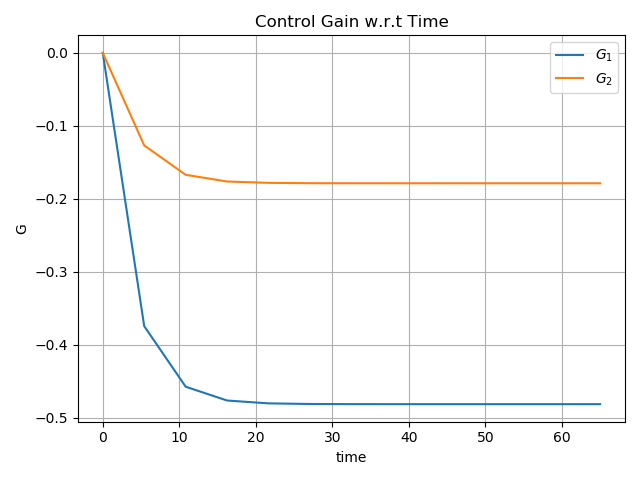
\includegraphics[width=1.0\textwidth]{Figures/G_t.png}
		\caption{Control gain $G$ w.r.t time\label{fig:G_t}}
	\end{minipage}
\end{figure}

\subsubsection{Numerical results}
\paragraph{Experiments with $n$}
With $n = 2000$, $\beta = 0.99$ (default value in PyTorch), $M = 8$, the ultimate $K$ is $[9.17\times 10^{-2}, 1.70\times 10^{-2}]^T$, and the ultimate $G$ is $[6.08\times 10^{-1}, -6.67\times 10^{-2}]$. The difference (in L2 norm) between the ultimate $K$ and the theoretical steady state $K$ is $2.49\times 10^{-2}$, and the difference (in L2 norm) between the ultimate $G$ and the theoretical steady state $G$ is $4.47\times 10^{-2}$. The cost simulating with the ultimate $K$, $G$ is $7.79\times 10^{-2}$, and testing the ultimate $K$, $G$ on 1000 simulations gives an expected cost of $6.94\times 10^{-2}$.\\
Figures \ref{fig:sgd_2000} to \ref{fig:diff_2000_sep} show the cost decay, the decay in the difference between $K$, $G$ and theoretical steady state $K$, $G$ in L2 norm, and the decay in the element-wise difference between $K$, $G$ and theoretical steady state $K$, $G$, respectively. \\
\begin{figure}[h!]
	\centering
	\begin{minipage}[t]{.27\paperwidth}
		\centering
		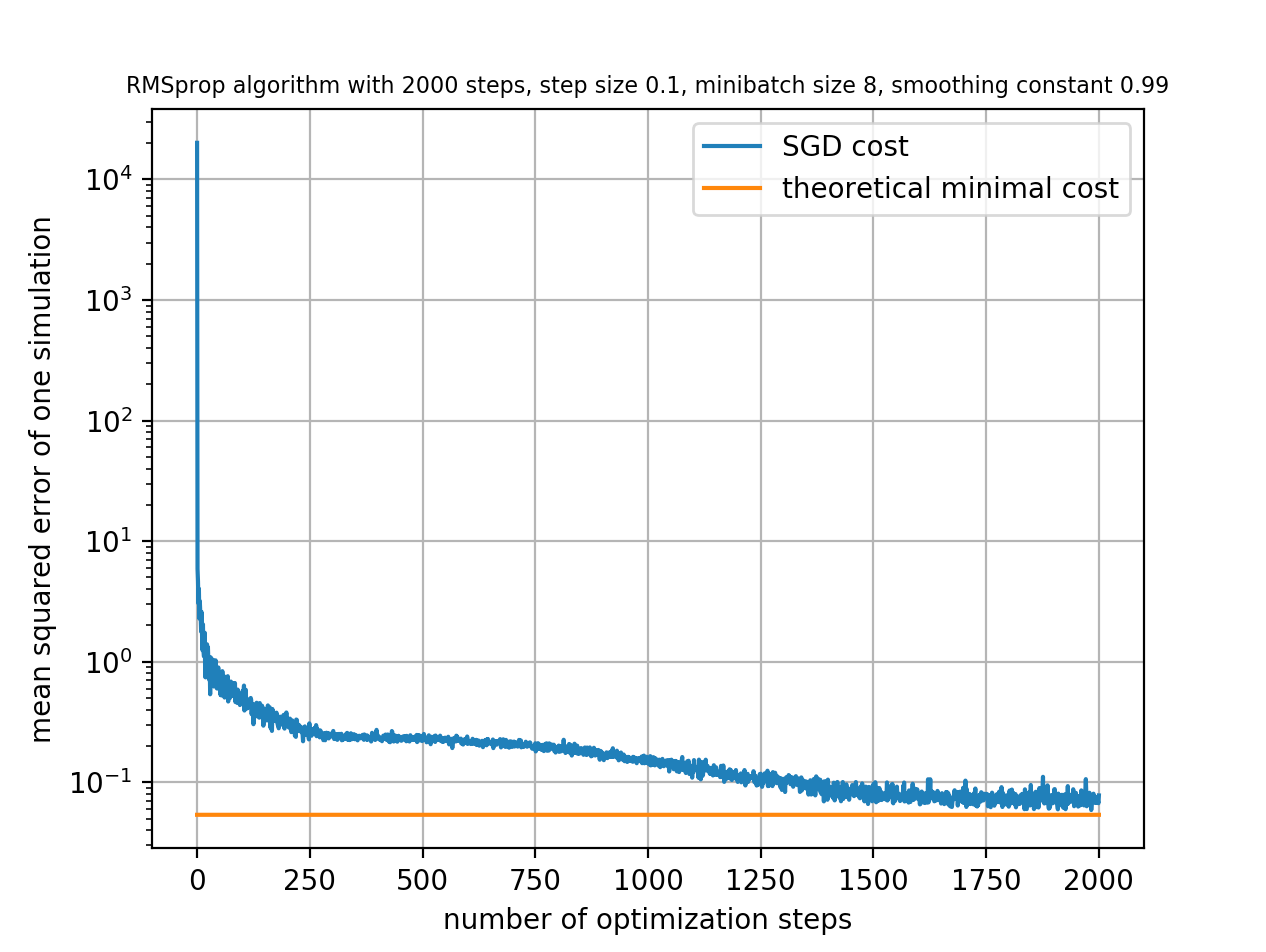
\includegraphics[width=1.0\textwidth]{Figures/sgd_2000.png}
		\caption{$n=2000$: cost w.r.t $n$\label{fig:sgd_2000}}
	\end{minipage}%
	\begin{minipage}[t]{.27\paperwidth}
		\centering
		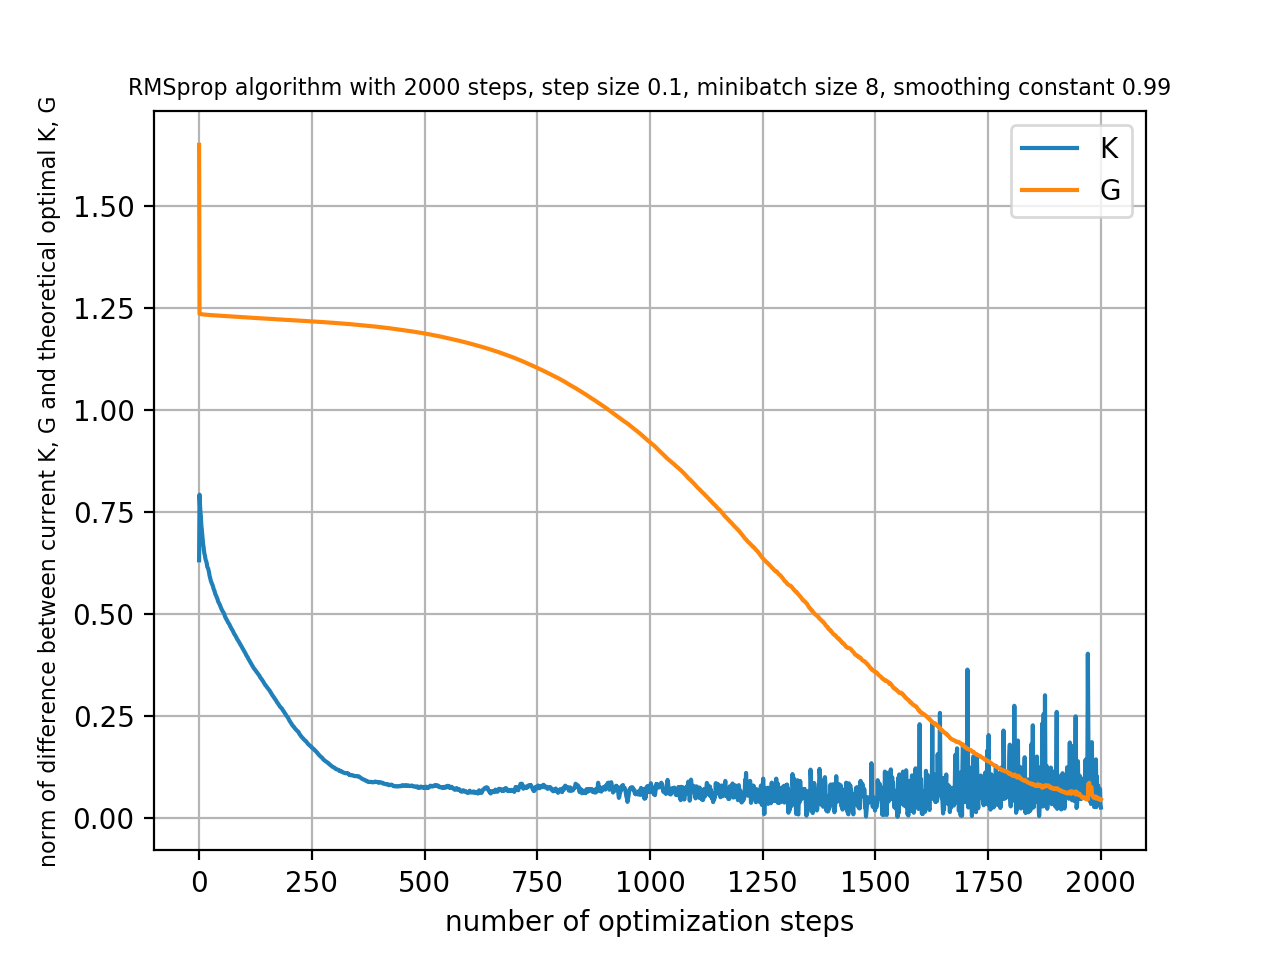
\includegraphics[width=1.0\textwidth]{Figures/diff_2000.png}
		\caption{$n=2000$: difference between $K$, $G$ and theoretical steady state $K$, $G$ w.r.t $n$\label{fig:diff_2000}}
	\end{minipage}%
	\begin{minipage}[t]{.27\paperwidth}
		\centering
		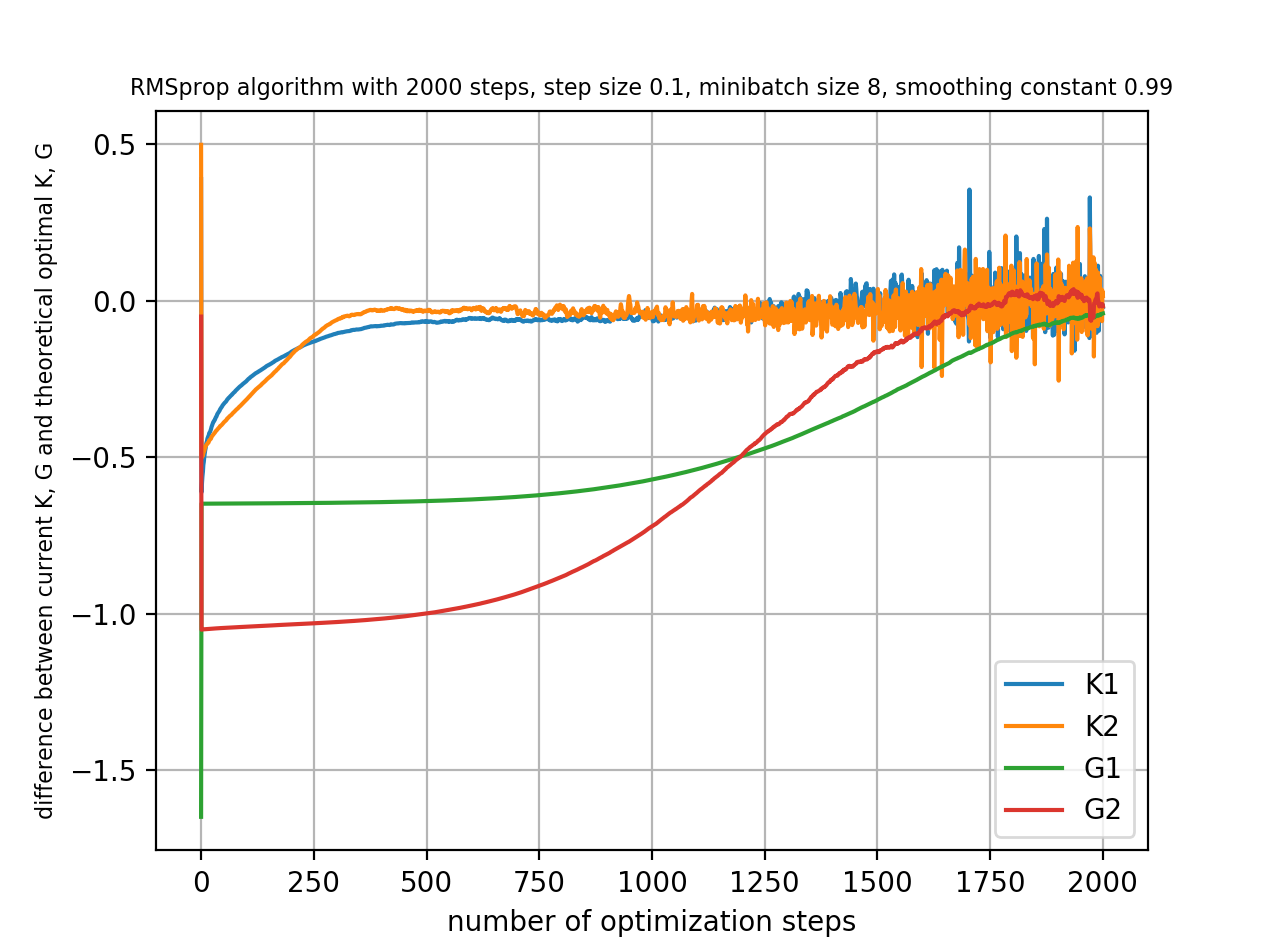
\includegraphics[width=1.0\textwidth]{Figures/diff_2000_sep.png}
		\caption{$n=2000$: difference between $K$, $G$ and theoretical steady state $K$, $G$ w.r.t $n$ (element-wise)\label{fig:diff_2000_sep}}
	\end{minipage}
\end{figure}

\noindent From the graphs, it seems that overall the numerical result converges to the theoretical steady result. However, there are noticeable fluctuations in the difference between the current $K$ and the theoretical steady state $K$ as we approaches 2000 iterations. The cause for these fluctuations may be that as we approach the optimum, the learning rate is too large so the result oscillates around the optimum. To further narrow down the difference between the numerical result and the theoretical result, we increase the number of iterations and use a learning rate scheduler to decay the learning rate manually. 

\noindent In particular, if we run 4000 iterations and use a learning rate scheduler to set $\alpha = 0.1\alpha$ after 2000 iterations and 3000 iterations, then the ultimate $K$ is $[8.41\times 10^{-2}, 1.70\times 10^{-3}]^T$, and the ultimate $G$ is $[6.45\times 10^{-1}, -5.35\times 10^{-2}]$. The differences between the ultimate $K$, $G$ and the theoretical steady state $K$, $G$ are $2.79\times 10^{-2}$ and $6.14\times 10^{-3}$, respectively. The cost simulating with the ultimate $K$, $G$ is $6.67\times 10^{-2}$, and testing the ultimate $K$, $G$ on 1000 simulations gives an expected cost of $6.97\times 10^{-2}$.\\
Figures \ref{fig:sgd_4000} to \ref{fig:diff_4000_sep} show the cost decay, the decay in the difference between $K$, $G$ and theoretical steady state $K$, $G$ in L2 norm, and the decay in the element-wise difference between $K$, $G$ and theoretical steady state $K$, $G$, respectively. \\
\begin{figure}[h!]
	\centering
	\begin{minipage}[t]{.27\paperwidth}
		\centering
		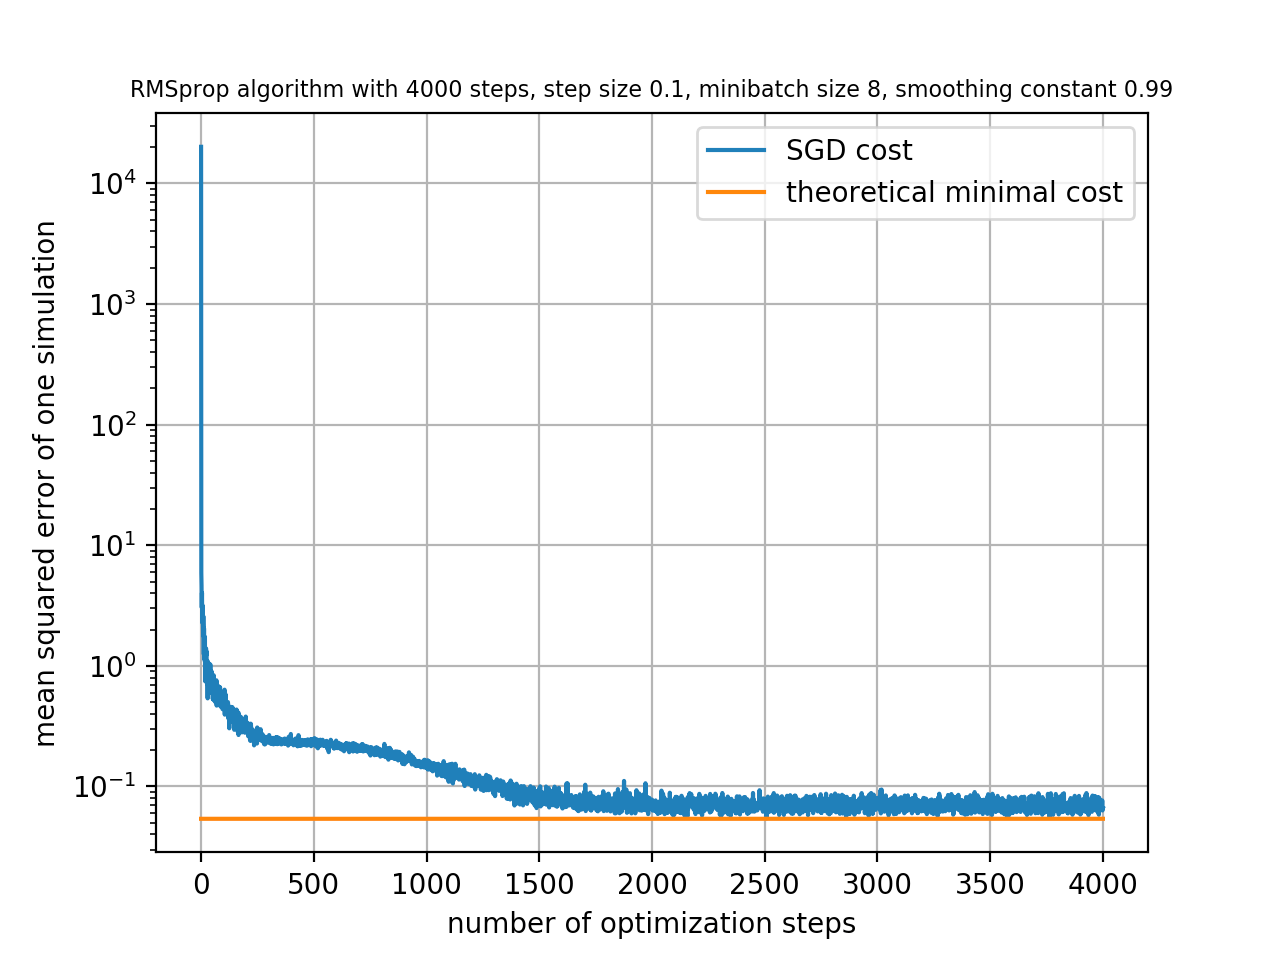
\includegraphics[width=1.0\textwidth]{Figures/sgd_4000.png}
		\caption{$n=4000$: cost w.r.t $n$\label{fig:sgd_4000}}
	\end{minipage}%
	\begin{minipage}[t]{.27\paperwidth}
		\centering
		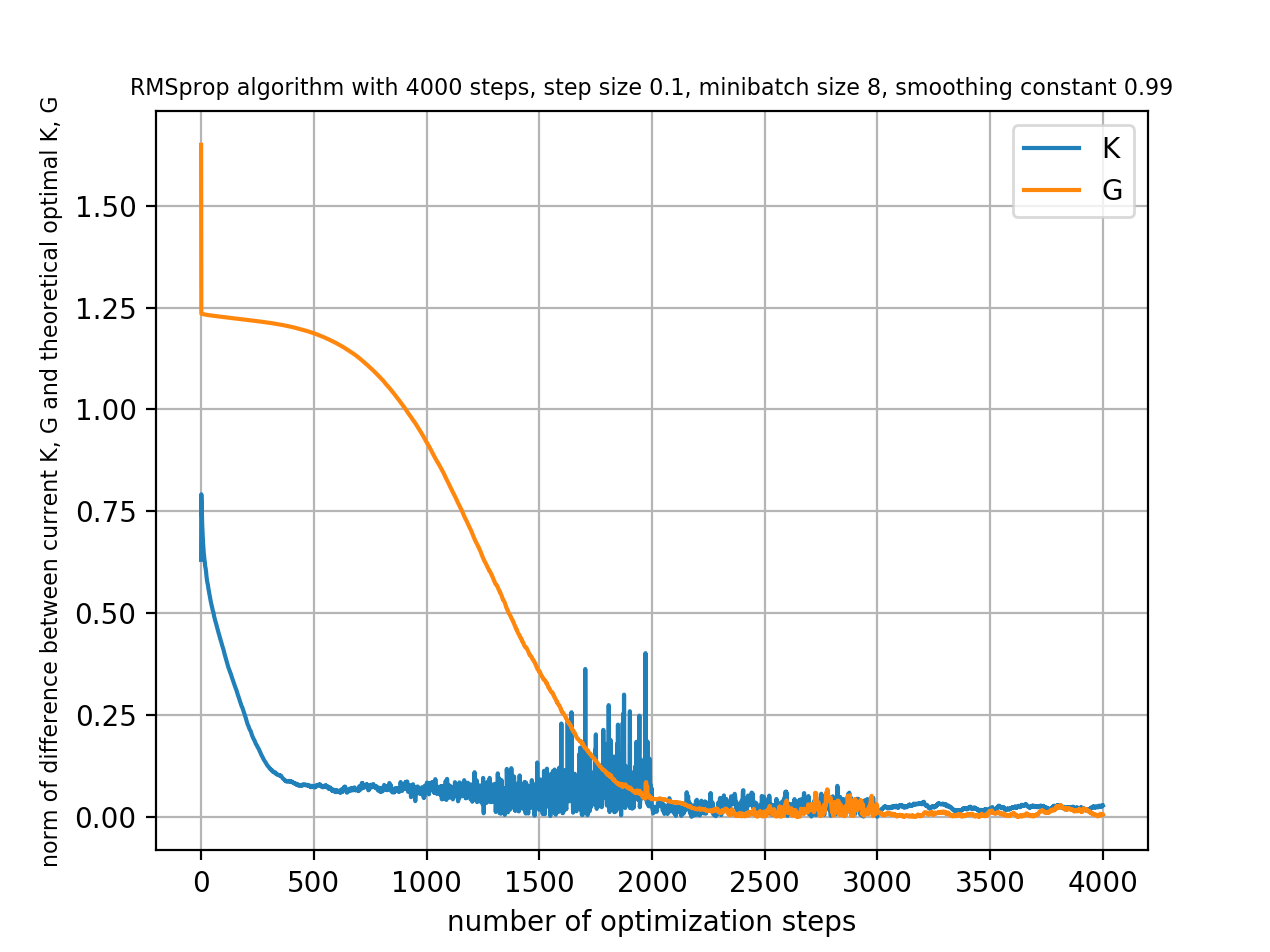
\includegraphics[width=1.0\textwidth]{Figures/diff_4000.png}
		\caption{$n=4000$: difference between $K$, $G$ and theoretical steady state $K$, $G$ w.r.t $n$\label{fig:diff_4000}}
	\end{minipage}%
	\begin{minipage}[t]{.27\paperwidth}
		\centering
		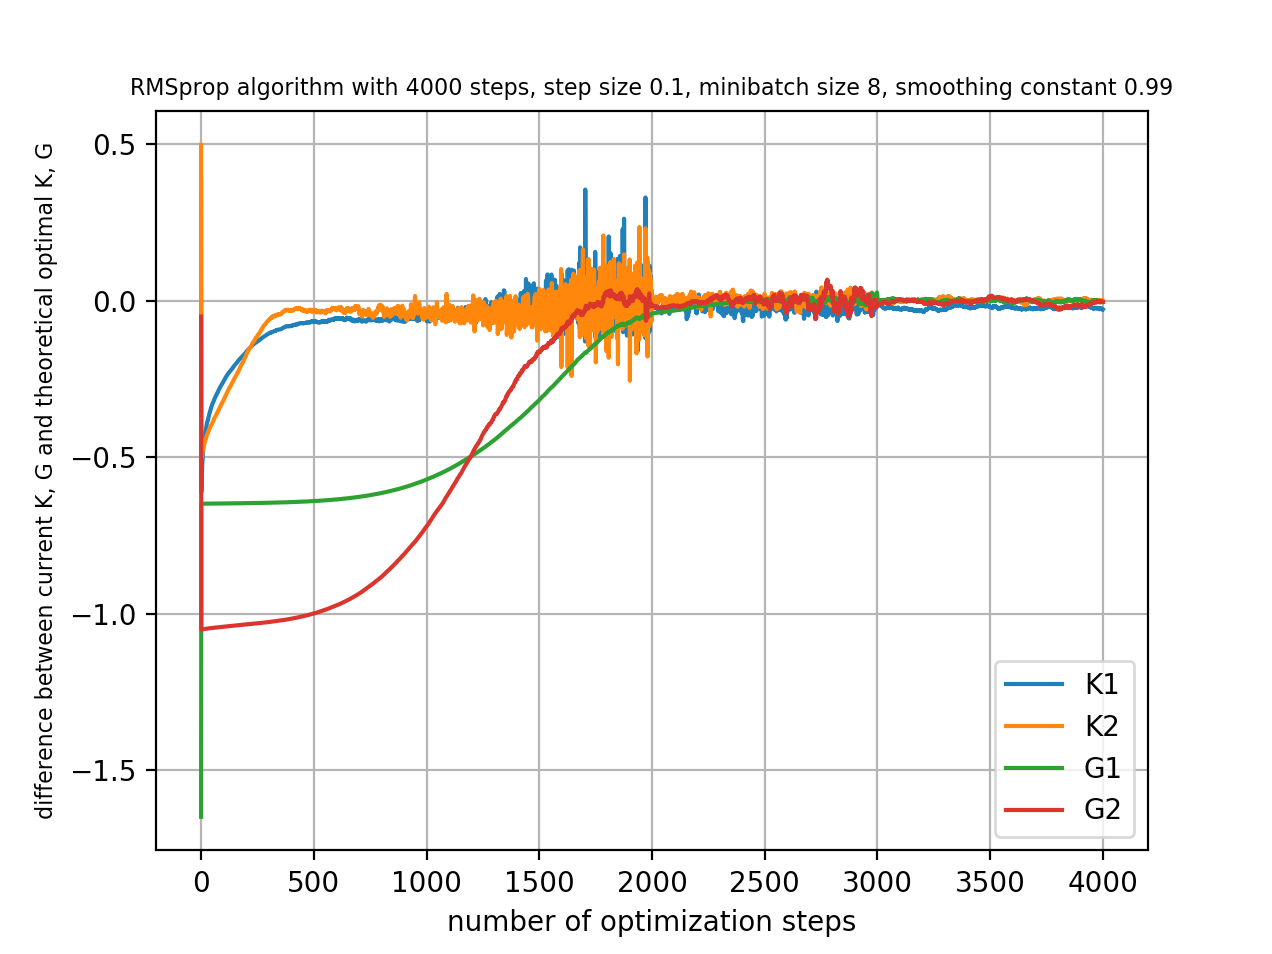
\includegraphics[width=1.0\textwidth]{Figures/diff_4000_sep.png}
		\caption{$n=4000$: difference between $K$, $G$ and theoretical steady state $K$, $G$ w.r.t $n$ (element-wise)\label{fig:diff_4000_sep}}
	\end{minipage}
\end{figure}

\paragraph{Experiments with $\beta$}
While the above experiments show that with a sufficiently large number of iterations and a sufficiently small learning rate, the result of RMSprop can eventually converge to the theoretical solution, we can't help wondering if there is a way to accelerate this convergence. It turns out that the smoothing constant $\beta$ plays a crucial role here. We observe that by decreasing $\beta$, we are able to achieve convergence within fewer iterations. Table \ref{table:2} compares the number of iterations that takes to converge for different $\beta$s when $\alpha = 0.1$ and $M = 8$. The first row in the table shows the theoretical result. Figures \ref{fig:beta_0_99} to \ref{fig:d_beta_0_sep} plot the decay in the cost, the decay in the difference between $K$, $G$ and theoretical steady state $K$, $G$ in L2 norm, and the decay in the element-wise difference between $K$, $G$ and theoretical steady state $K$, $G$ w.r.t. $n$ for different $\beta$s. Figure \ref{fig:comp_beta} offers a more intuitive comparison of the performances of different $\beta$s. From the results it seems that smaller $\beta$ can achieve faster convergence. This is especially surprising because when $\beta$ equals to 0, the algorithm is simply clipping the gradient to 1. However, we also note that although the convergence is fast when $\beta = 0$, the final cost and testing cost in this case is relatively large, which may be a drawback of doing simple gradient clipping. On the other hand, the poor performance of $\beta = 0.99$ indicates that it is probably not a good idea to rely too heavily on the past gradients.  \\
\begin{table}[h!]
	\begin{center}
		\begin{tabular}{|c|c|m{3.0cm}|m{3.0cm}|m{1.7cm}|m{1.7cm}|c|c|} 
			\hline
			$\beta$ & $n$ & ultimate $K$ & ultimate $G^T$ & final $K$ difference & final $G$ difference & final cost & testing cost \\ 
			\hline
			- & - & $\begin{bmatrix}1.12\times 10^{-1} \\ 2.44\times 10^{-3}\end{bmatrix}$ & $\begin{bmatrix}6.49\times 10^{-1} \\ -4.89\times 10^{-2}\end{bmatrix}$ & -- & -- & -- & $5.37\times 10^{-2}$\\
			\hline
			\hline
			0.99 & 400 & $\begin{bmatrix}3.18\times 10^{-2} \\ -2.89\times 10^{-2}\end{bmatrix}$ & $\begin{bmatrix}5.04\times 10^{-3} \\ -1.07\times 10^{0}\end{bmatrix}$ & $8.60\times 10^{-2}$ & $1.20\times 10^{0}$ & $2.36\times 10^{-1}$ & $2.35\times 10^{-1}$\\ 
			\hline
			0.9  & 400 & $\begin{bmatrix}1.13\times 10^{-1} \\ 1.91\times 10^{-2}\end{bmatrix}$ & $\begin{bmatrix}6.11\times 10^{-1} \\ -1.28\times 10^{-1}\end{bmatrix}$ & $1.67\times 10^{-2}$ & $8.81\times 10^{-2}$ & $7.45\times 10^{-2}$ & $7.01\times 10^{-2}$\\ 
			\hline
			0.85  & 300 & $\begin{bmatrix}8.57\times 10^{-2} \\ 5.60\times 10^{-2}\end{bmatrix}$ & $\begin{bmatrix}6.30\times 10^{-1} \\ -1.00\times 10^{-1}\end{bmatrix}$ & $5.97\times 10^{-2}$ & $5.45\times 10^{-2}$ & $7.52\times 10^{-2}$ & $6.95\times 10^{-2}$\\ 
			\hline
			0.75 & 300 & $\begin{bmatrix}8.88\times 10^{-2} \\ 6.72\times 10^{-2}\end{bmatrix}$ & $\begin{bmatrix}6.40\times 10^{-1} \\ -9.95\times 10^{-2}\end{bmatrix}$ & $6.88\times 10^{-2}$ & $5.13\times 10^{-2}$ & $7.51\times 10^{-2}$ & $6.99\times 10^{-2}$\\ 
			\hline
			0.5 & 200 & $\begin{bmatrix}9.04\times 10^{-2} \\ -1.33\times 10^{-2}\end{bmatrix}$ & $\begin{bmatrix}6.37\times 10^{-1} \\ -1.70\times 10^{-2}\end{bmatrix}$ & $2.67\times 10^{-2}$ & $3.40\times 10^{-2}$ & $7.51\times 10^{-2}$ & $6.96\times 10^{-2}$\\
			\hline
			0.25 & 200 & $\begin{bmatrix}8.16\times 10^{-2} \\ -1.30\times 10^{-2}\end{bmatrix}$ & $\begin{bmatrix}6.19\times 10^{-1} \\ 1.45\times 10^{-2}\end{bmatrix}$ & $3.40\times 10^{-2}$ & $6.99\times 10^{-2}$ & $7.53\times 10^{-2}$ & $6.97\times 10^{-2}$\\ 
			\hline
			0.00 & 200 & $\begin{bmatrix}1.00\times 10^{-1} \\ 1.00\times 10^{-1}\end{bmatrix}$ & $\begin{bmatrix}6.00\times 10^{-1} \\ -1.00\times 10^{-1}\end{bmatrix}$ & $9.83\times 10^{-2}$ & $7.05\times 10^{-2}$ & $7.63\times 10^{-2}$ & $7.26\times 10^{-2}$\\ 
			\hline
		\end{tabular}
	\end{center}
	\caption{Comparison of different $\beta$}
	\label{table:2}
\end{table}
\begin{figure}[h!]
	\centering
	\begin{minipage}[t]{.28\paperwidth}
		\centering
		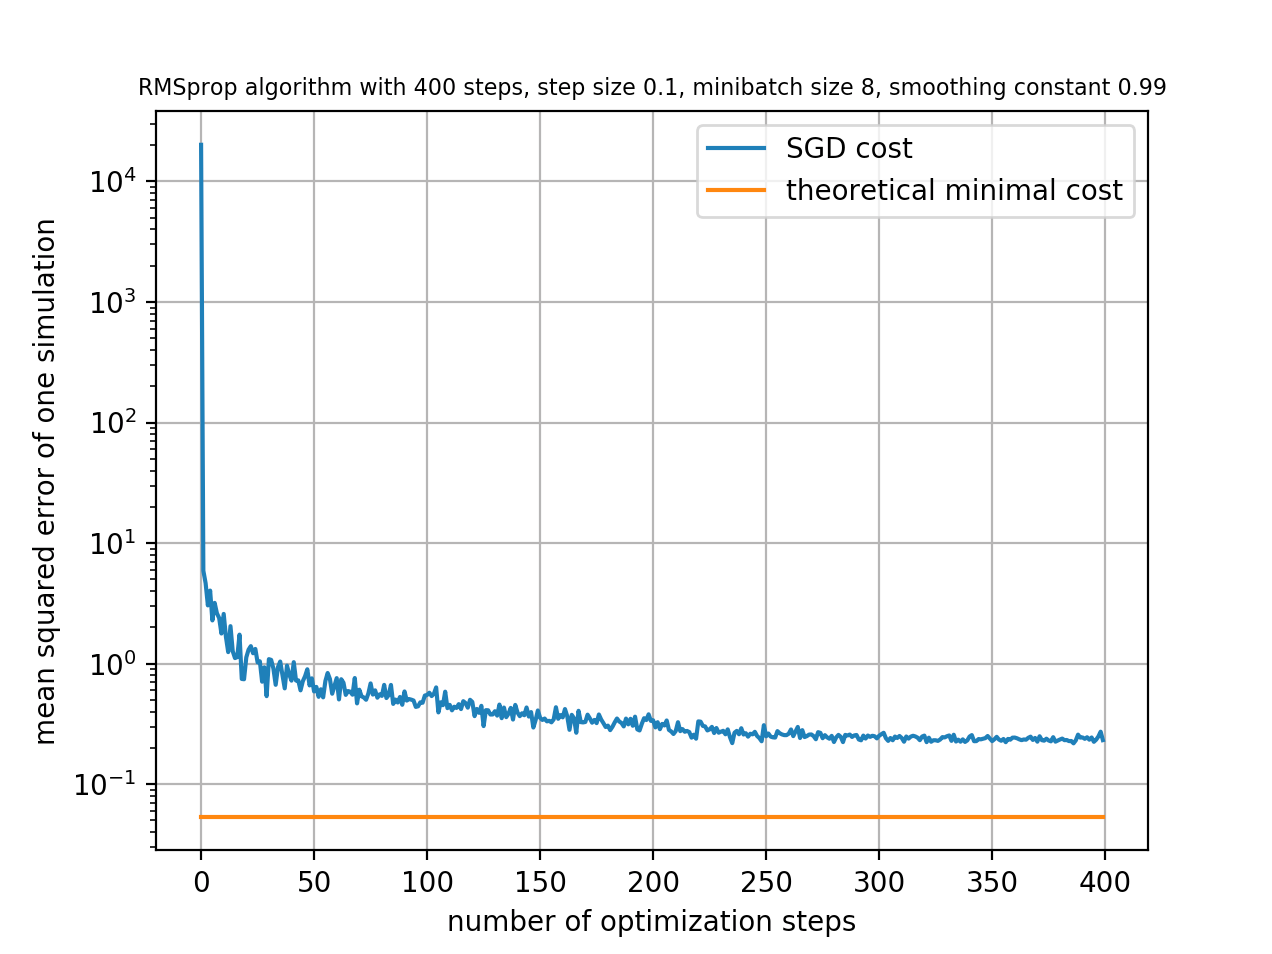
\includegraphics[width=1.0\textwidth]{Figures/beta_0_99.png}
		\caption{$\beta = 0.99$: cost w.r.t $n$\label{fig:beta_0_99}}
	\end{minipage}%
	\begin{minipage}[t]{.28\paperwidth}
		\centering
		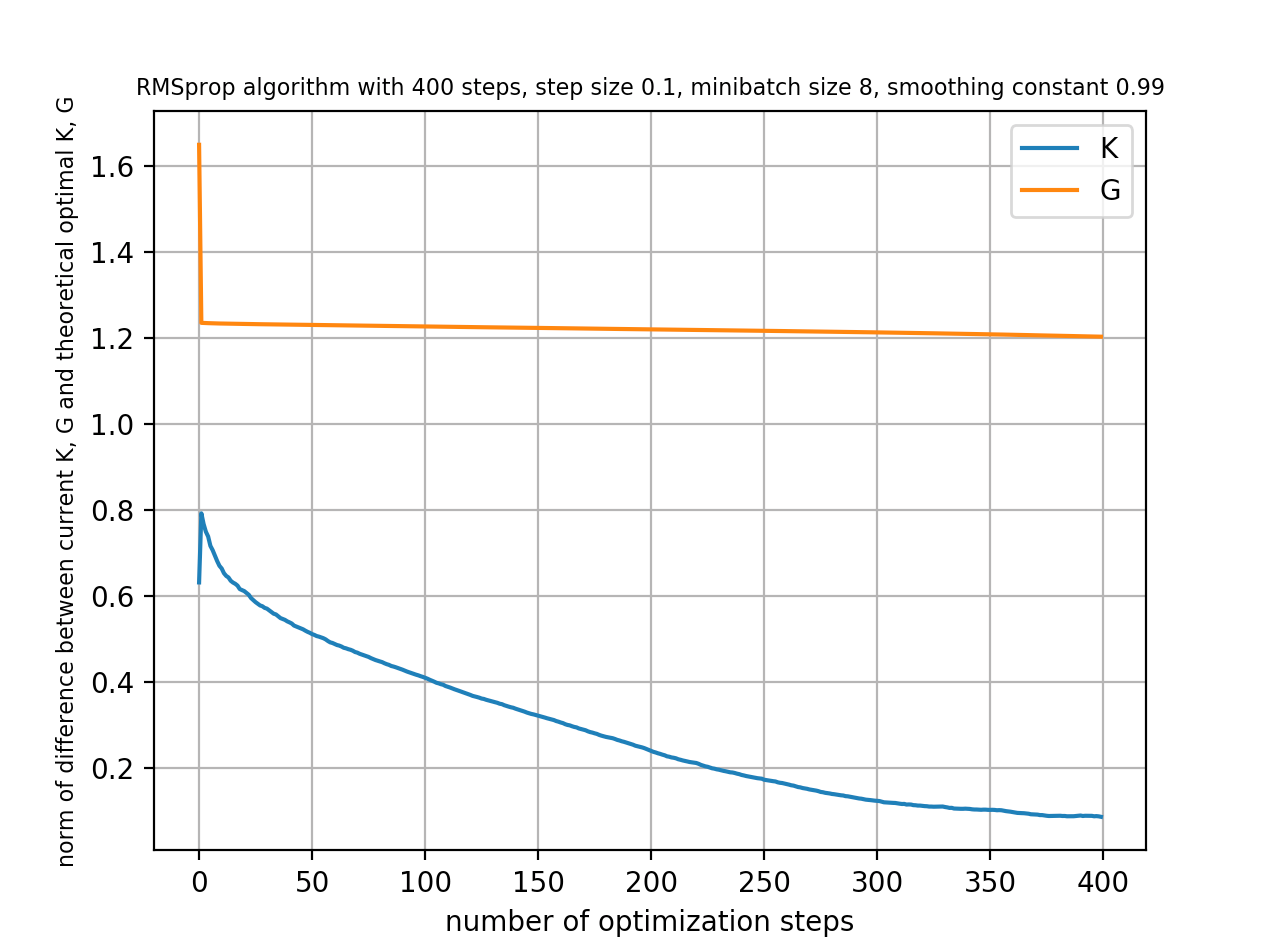
\includegraphics[width=1.0\textwidth]{Figures/d_beta_0_99.png}
		\caption{$\beta = 0.99$: difference between $K$, $G$ and theoretical steady state $K$, $G$ w.r.t $n$}
	\end{minipage}%
	\begin{minipage}[t]{.28\paperwidth}
		\centering
		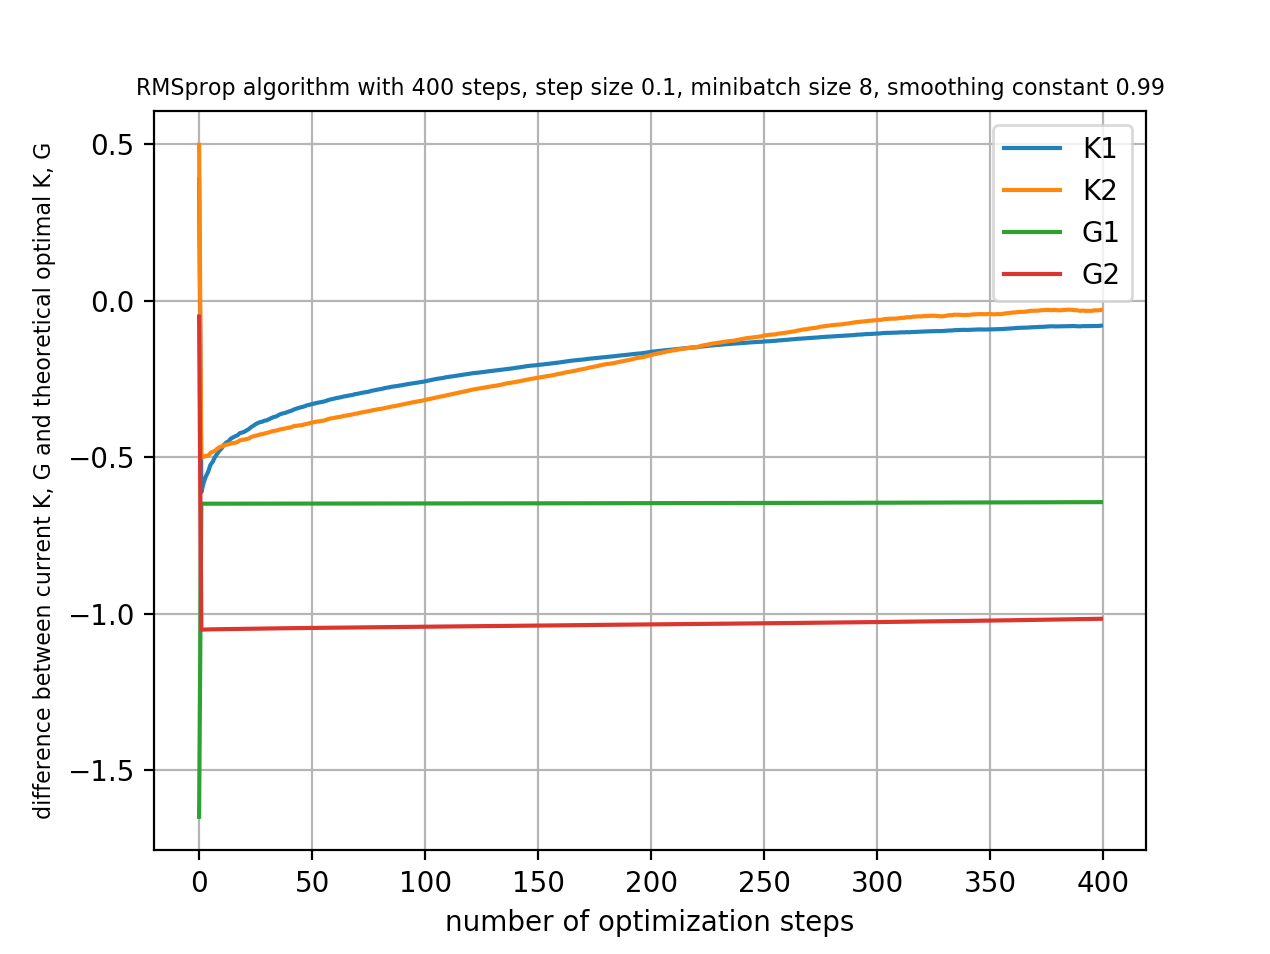
\includegraphics[width=1.0\textwidth]{Figures/d_beta_0_99_sep.png}
		\caption{$\beta = 0.99$: difference between $K$, $G$ and theoretical steady state $K$, $G$ w.r.t $n$ (element-wise)}
	\end{minipage}
\end{figure}
\begin{figure}[h!]
	\centering
	\begin{minipage}[t]{.28\paperwidth}
		\centering
		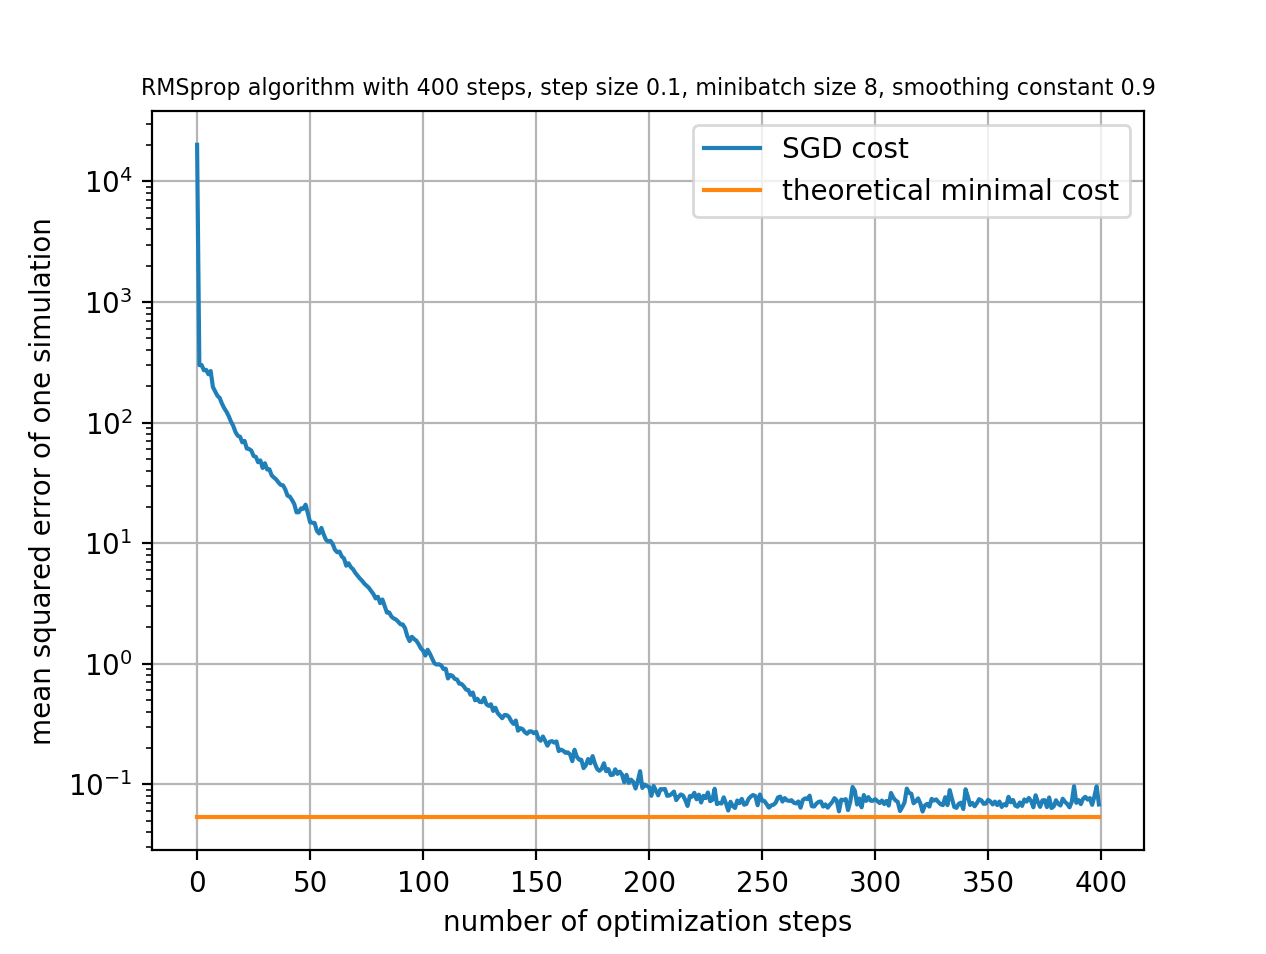
\includegraphics[width=1.0\textwidth]{Figures/beta0_9.png}
		\caption{$\beta = 0.9$: cost w.r.t $n$}
	\end{minipage}%
	\begin{minipage}[t]{.28\paperwidth}
		\centering
		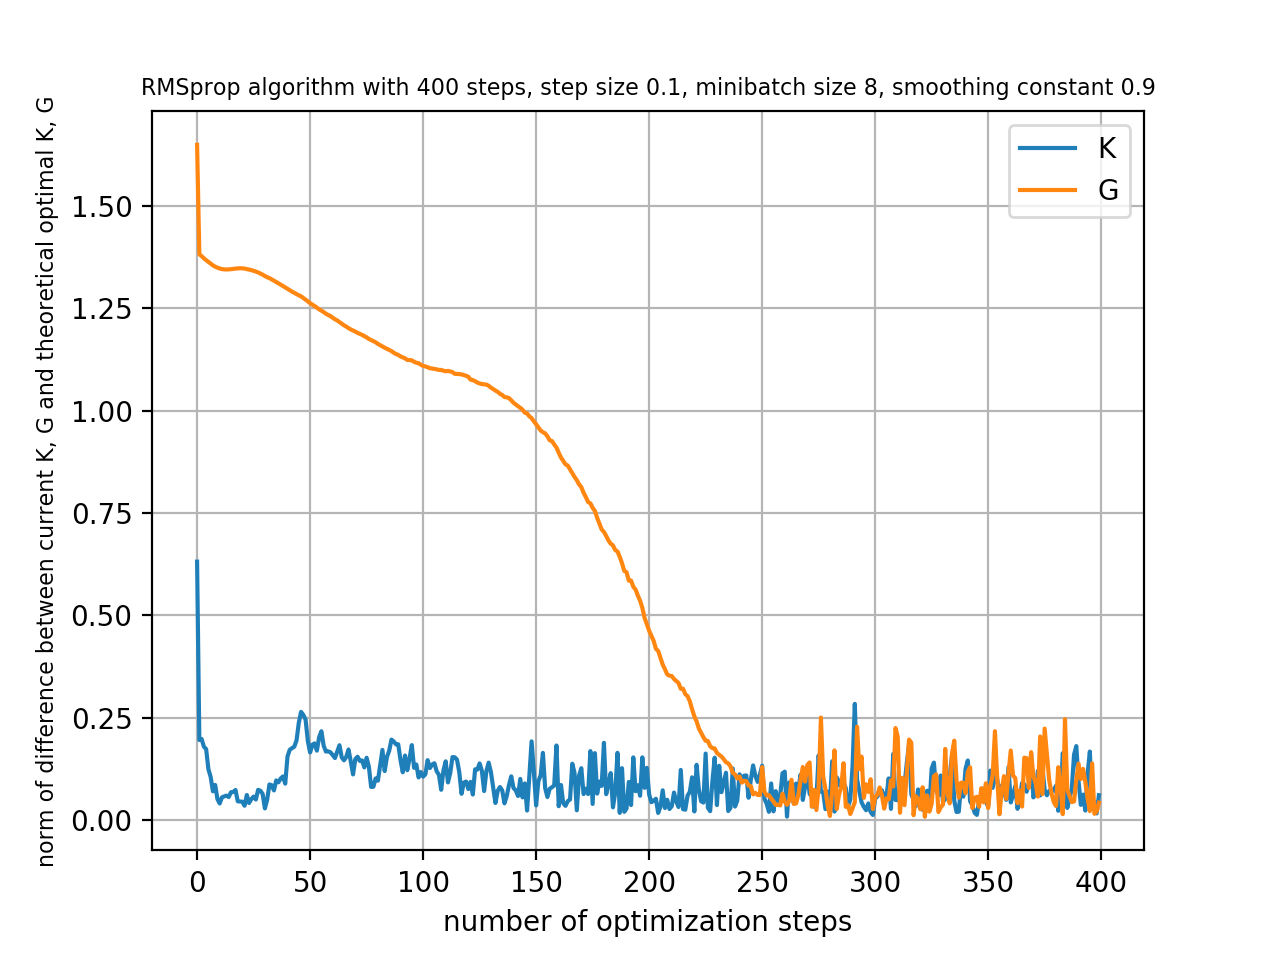
\includegraphics[width=1.0\textwidth]{Figures/d_beta_0_9.png}
		\caption{$\beta = 0.9$: difference between $K$, $G$ and theoretical steady state $K$, $G$ w.r.t $n$}
	\end{minipage}%
	\begin{minipage}[t]{.28\paperwidth}
		\centering
		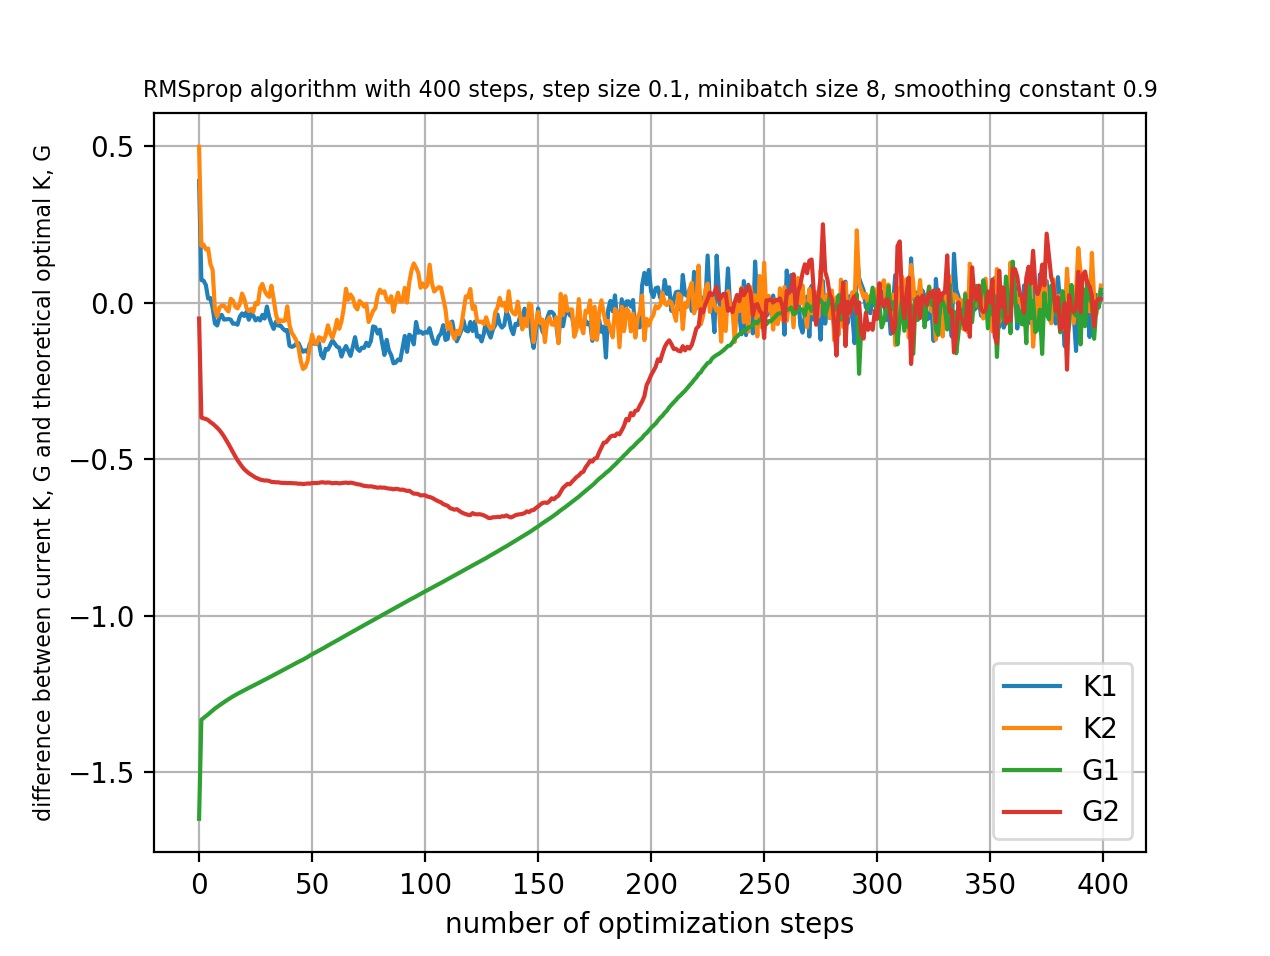
\includegraphics[width=1.0\textwidth]{Figures/d_beta_0_9_sep.png}
		\caption{$\beta = 0.9$: difference between $K$, $G$ and theoretical steady state $K$, $G$ w.r.t $n$ (element-wise)}
	\end{minipage}
\end{figure}
\begin{figure}[h!]
	\centering
	\begin{minipage}[t]{.28\paperwidth}
		\centering
		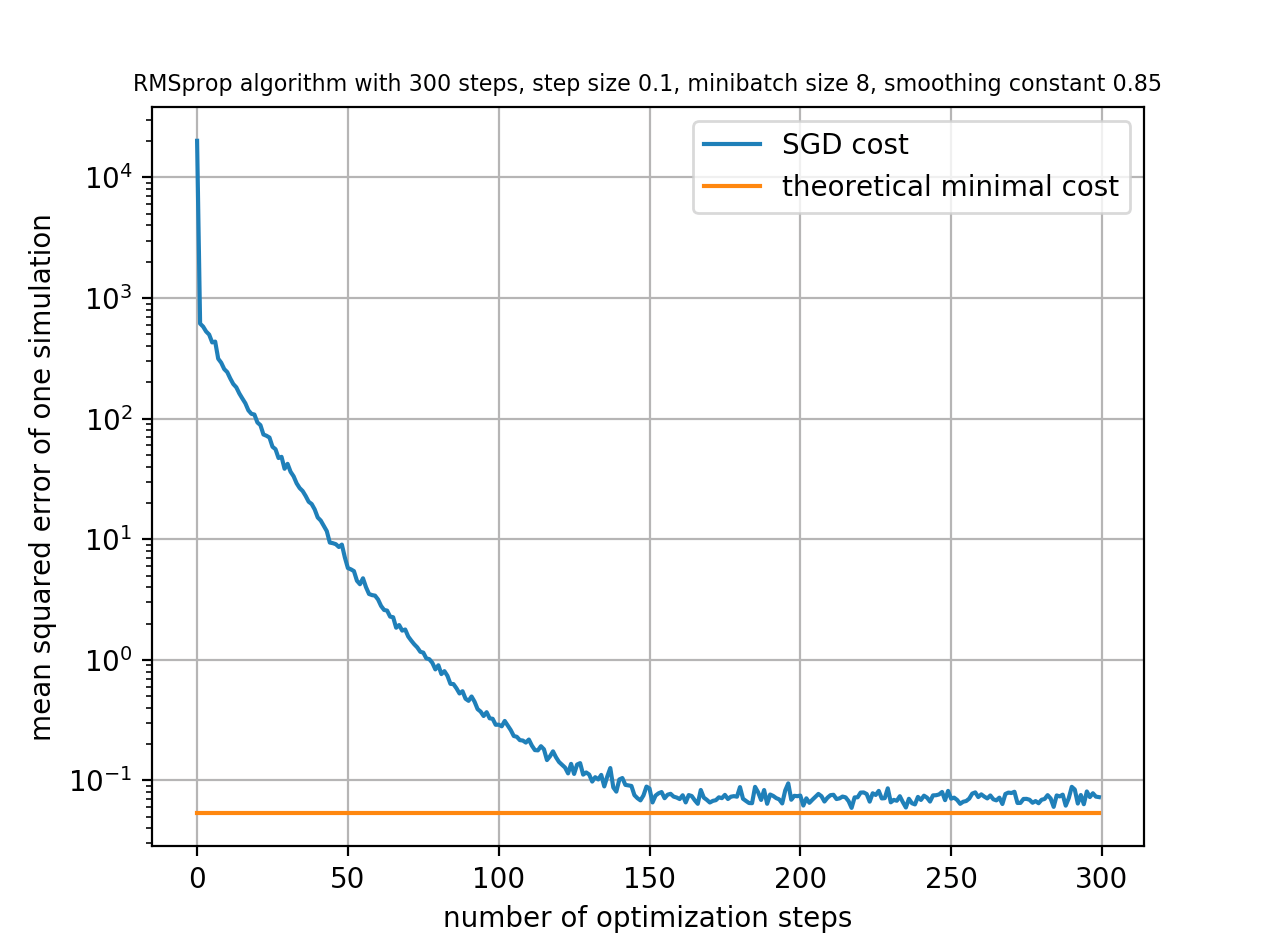
\includegraphics[width=1.0\textwidth]{Figures/beta0_85.png}
		\caption{$\beta = 0.85$: cost w.r.t $n$}
	\end{minipage}%
	\begin{minipage}[t]{.28\paperwidth}
		\centering
		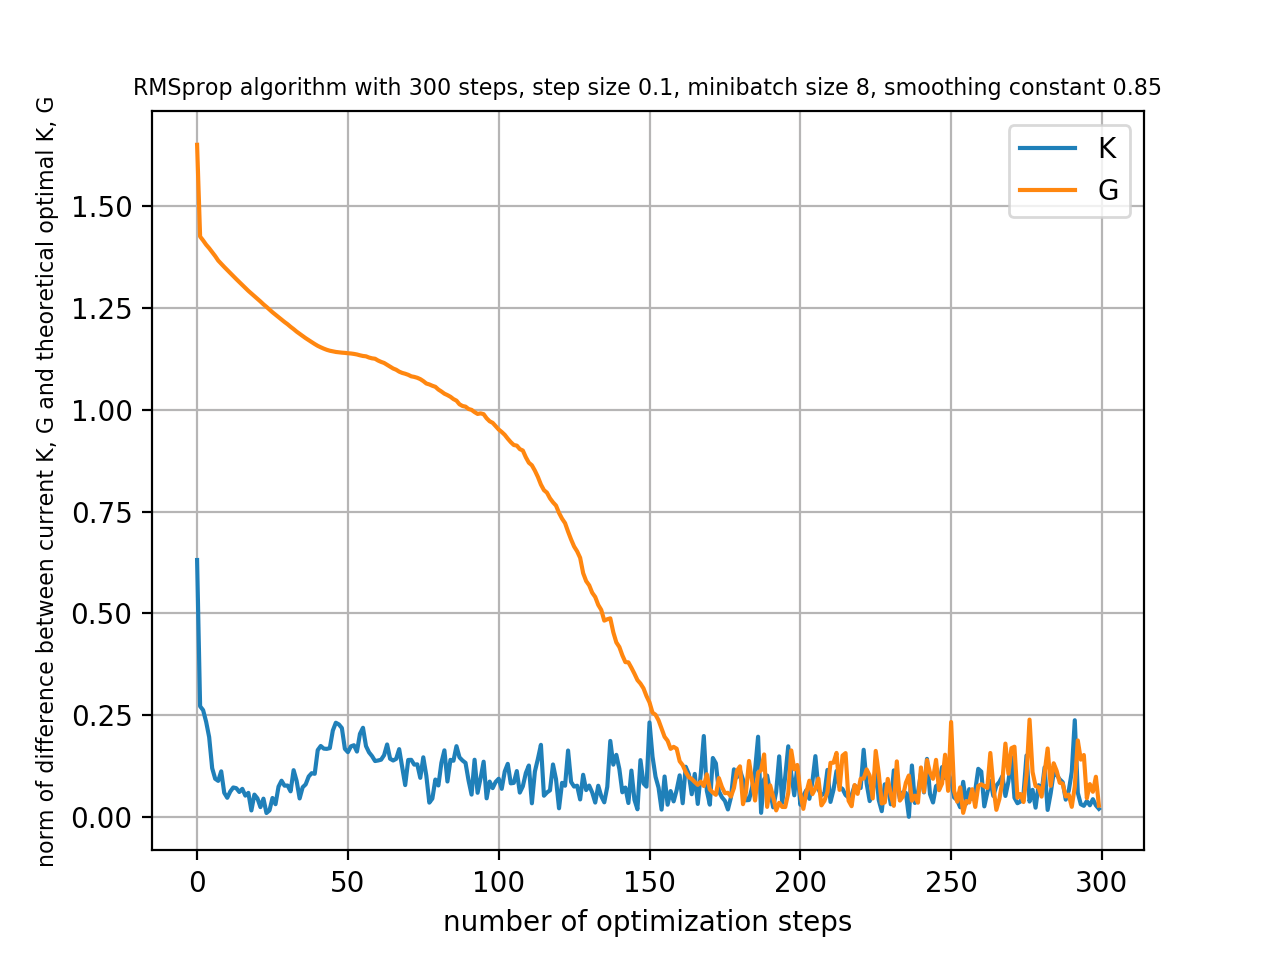
\includegraphics[width=1.0\textwidth]{Figures/d_beta_0_85.png}
		\caption{$\beta = 0.85$: difference between $K$, $G$ and theoretical steady state $K$, $G$ w.r.t $n$}
	\end{minipage}%
	\begin{minipage}[t]{.28\paperwidth}
		\centering
		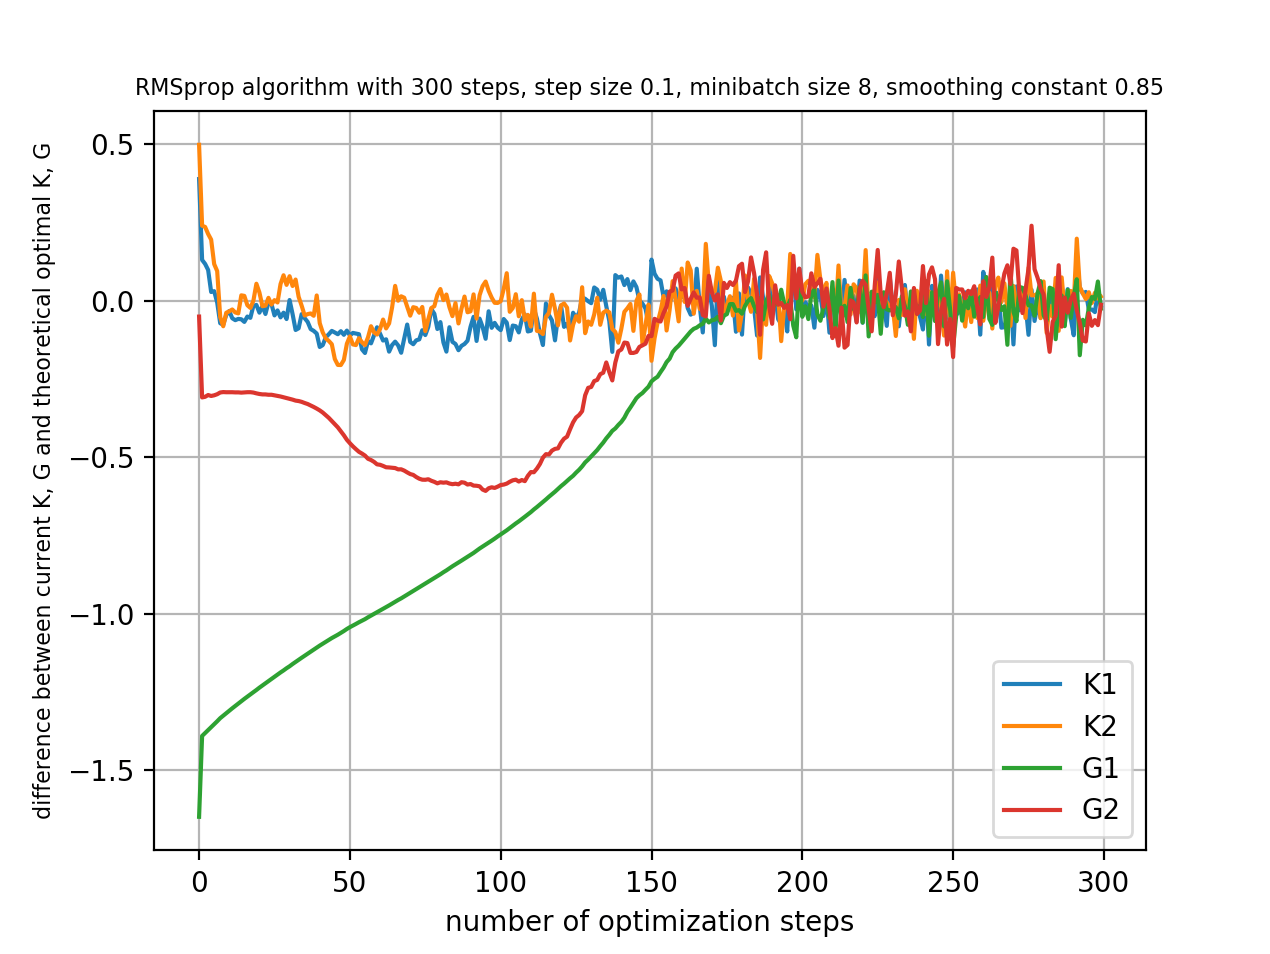
\includegraphics[width=1.0\textwidth]{Figures/d_beta_0_85_sep.png}
		\caption{$\beta = 0.85$: difference between $K$, $G$ and theoretical steady state $K$, $G$ w.r.t $n$ (element-wise)}
	\end{minipage}
\end{figure}
\begin{figure}[h!]
	\centering
	\begin{minipage}[t]{.28\paperwidth}
		\centering
		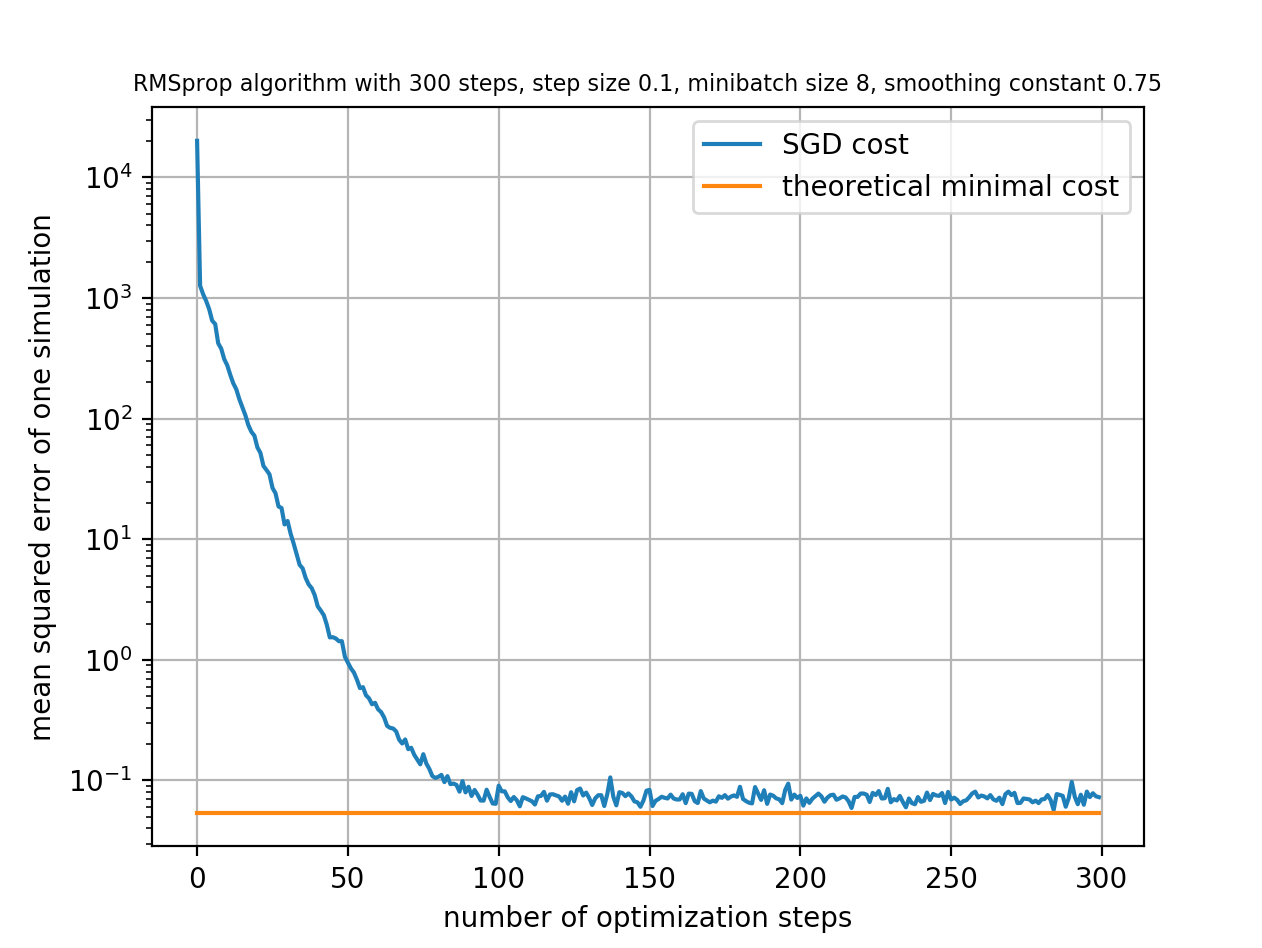
\includegraphics[width=1.0\textwidth]{Figures/beta_0_75.png}
		\caption{$\beta = 0.75$: cost w.r.t $n$}
	\end{minipage}%
	\begin{minipage}[t]{.28\paperwidth}
		\centering
		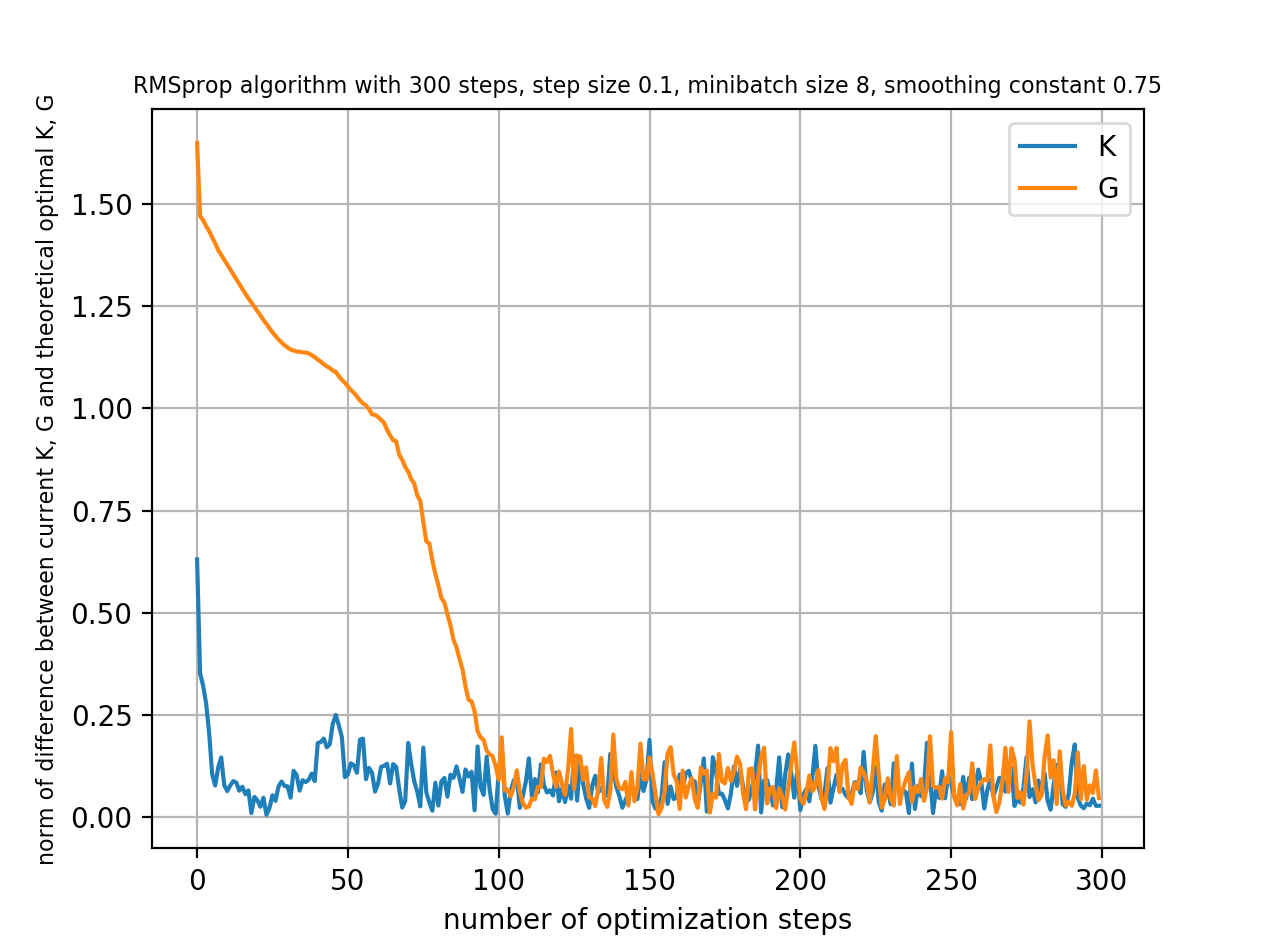
\includegraphics[width=1.0\textwidth]{Figures/d_beta_0_75.png}
		\caption{$\beta = 0.75$: difference between $K$, $G$ and theoretical steady state $K$, $G$ w.r.t $n$}
	\end{minipage}%
	\begin{minipage}[t]{.28\paperwidth}
		\centering
		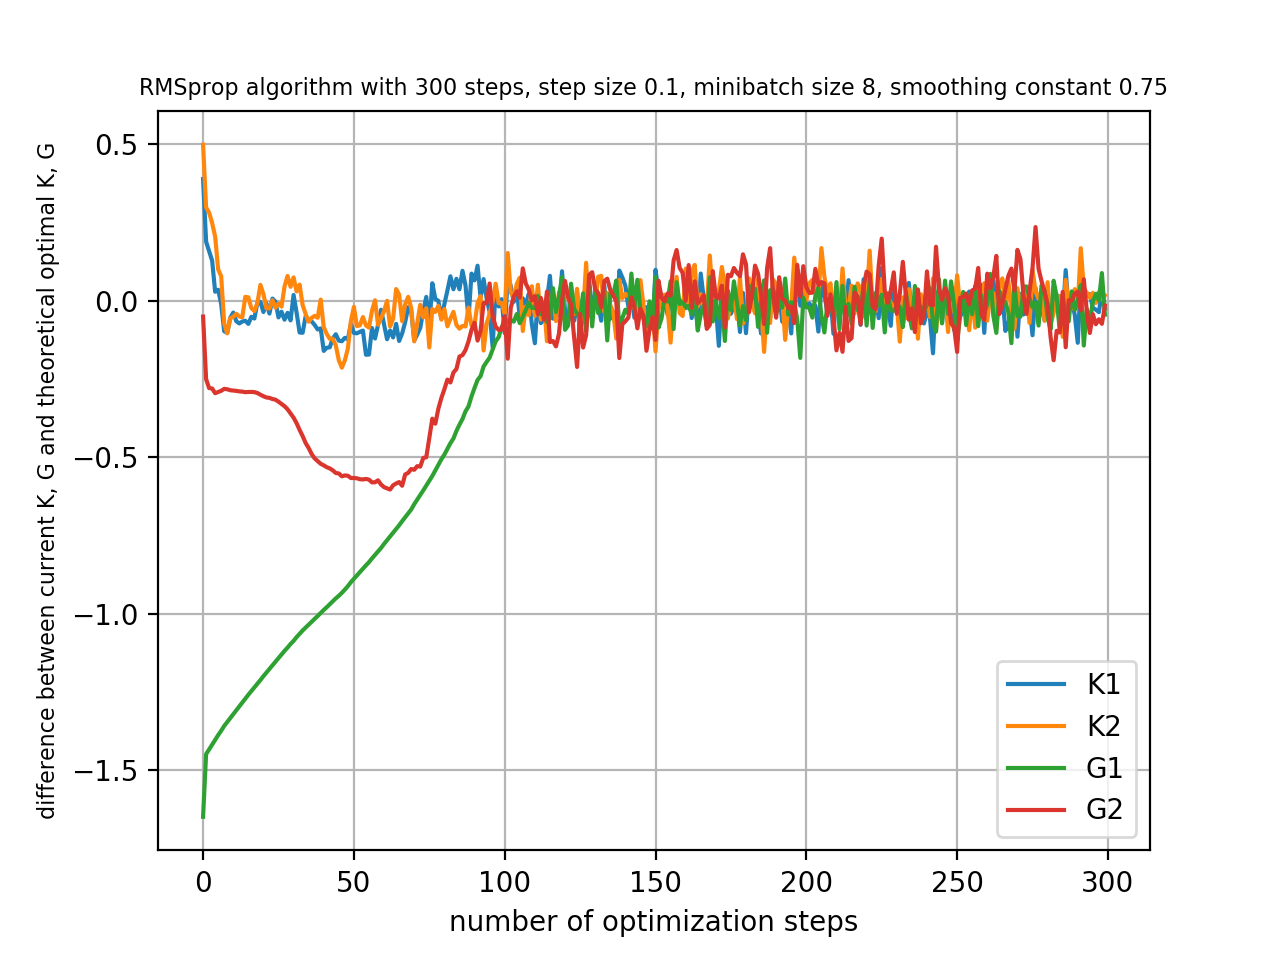
\includegraphics[width=1.0\textwidth]{Figures/d_beta_0_75_sep.png}
		\caption{$\beta = 0.75$: difference between $K$, $G$ and theoretical steady state $K$, $G$ w.r.t $n$ (element-wise)}
	\end{minipage}
\end{figure}
\begin{figure}[h!]
	\centering
	\begin{minipage}[t]{.28\paperwidth}
		\centering
		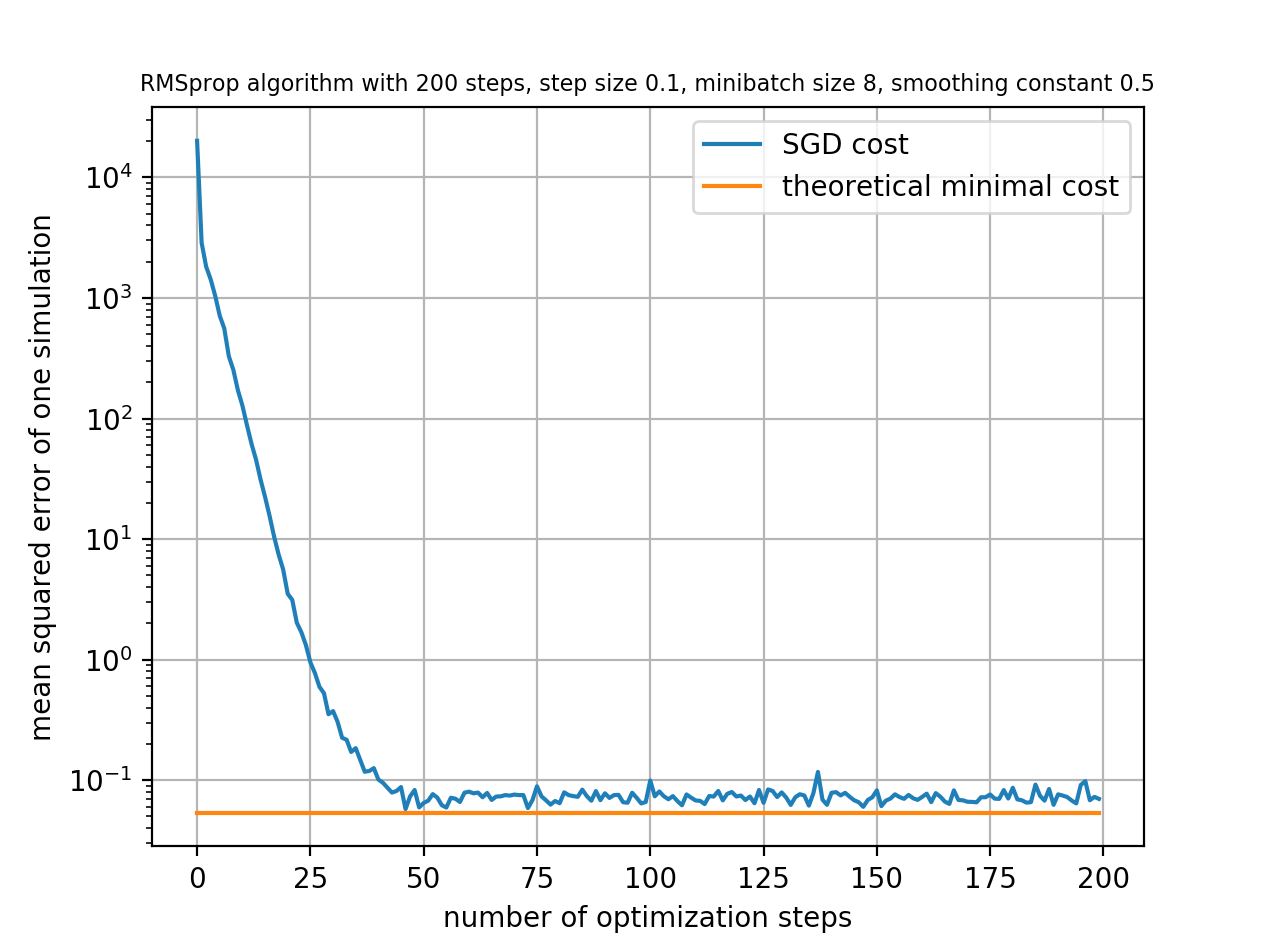
\includegraphics[width=1.0\textwidth]{Figures/beta_0_5.png}
		\caption{$\beta = 0.5$: cost w.r.t $n$}
	\end{minipage}%
	\begin{minipage}[t]{.28\paperwidth}
		\centering
		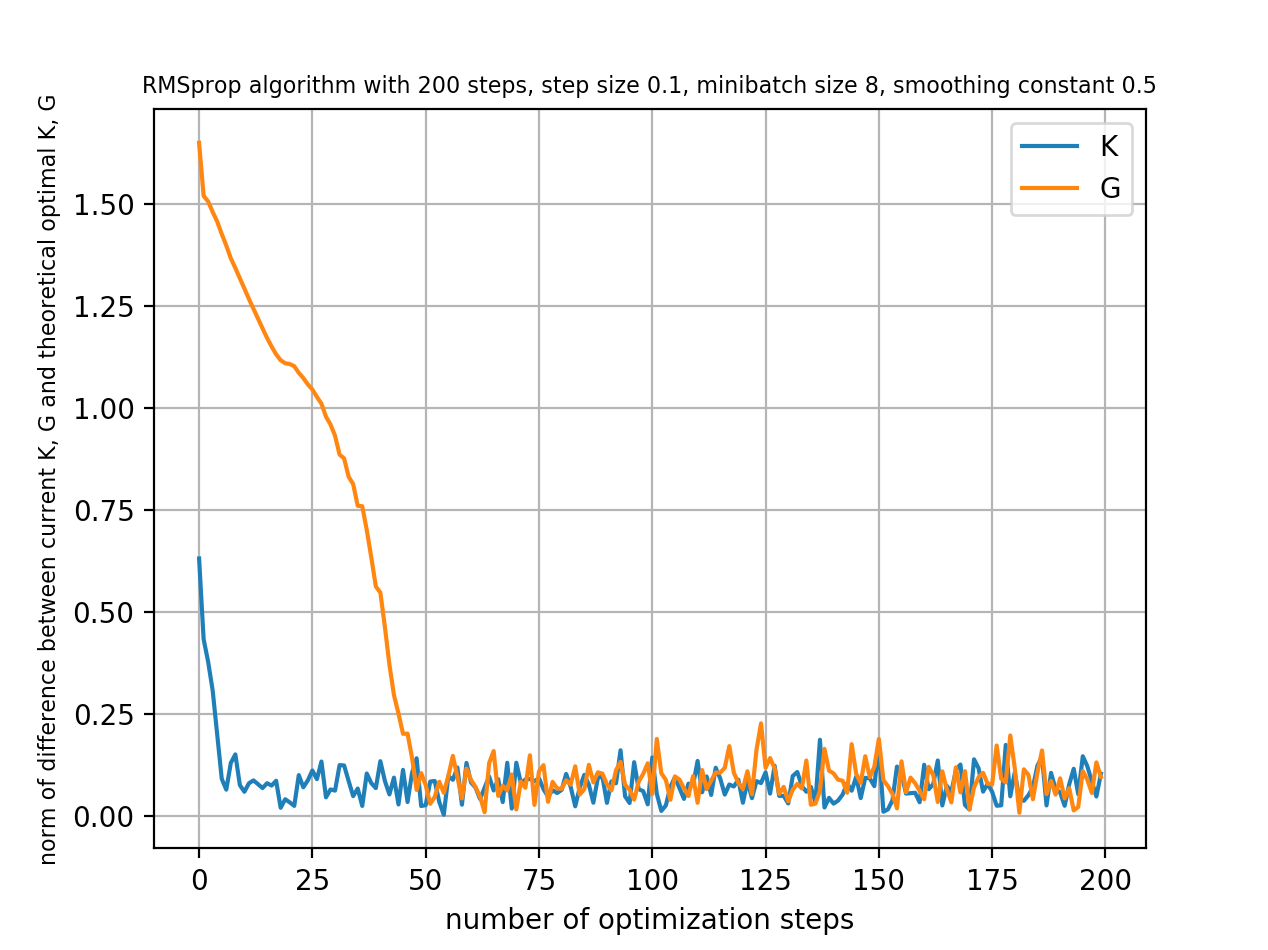
\includegraphics[width=1.0\textwidth]{Figures/d_beta_0_5.png}
		\caption{$\beta = 0.5$: difference between $K$, $G$ and theoretical steady state $K$, $G$ w.r.t $n$}
	\end{minipage}%
	\begin{minipage}[t]{.28\paperwidth}
		\centering
		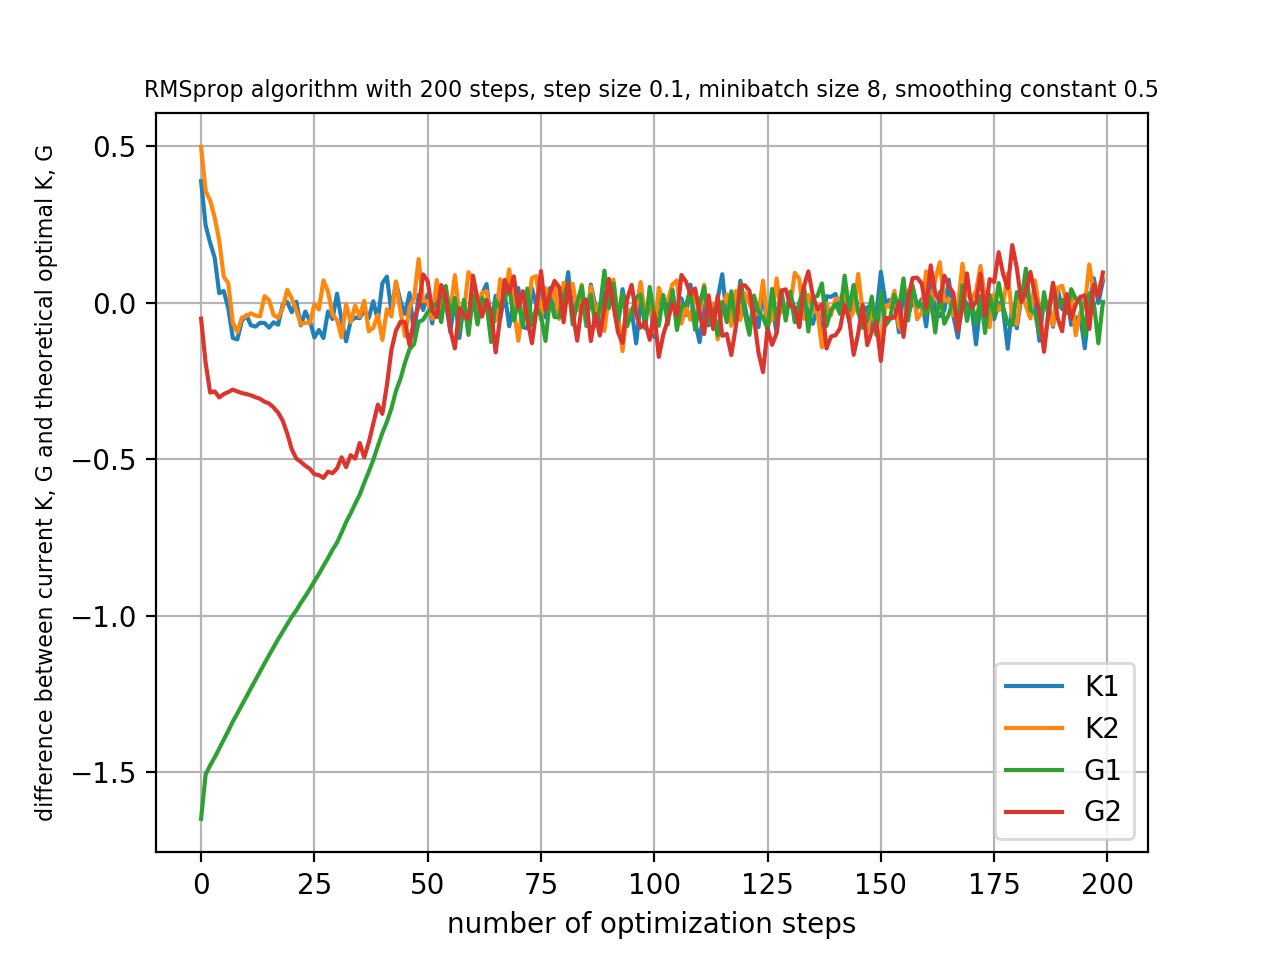
\includegraphics[width=1.0\textwidth]{Figures/d_beta_0_5_sep.png}
		\caption{$\beta = 0.5$: difference between $K$, $G$ and theoretical steady state $K$, $G$ w.r.t $n$ (element-wise)}
	\end{minipage}
\end{figure}
\begin{figure}[h!]
	\centering
	\begin{minipage}[t]{.28\paperwidth}
		\centering
		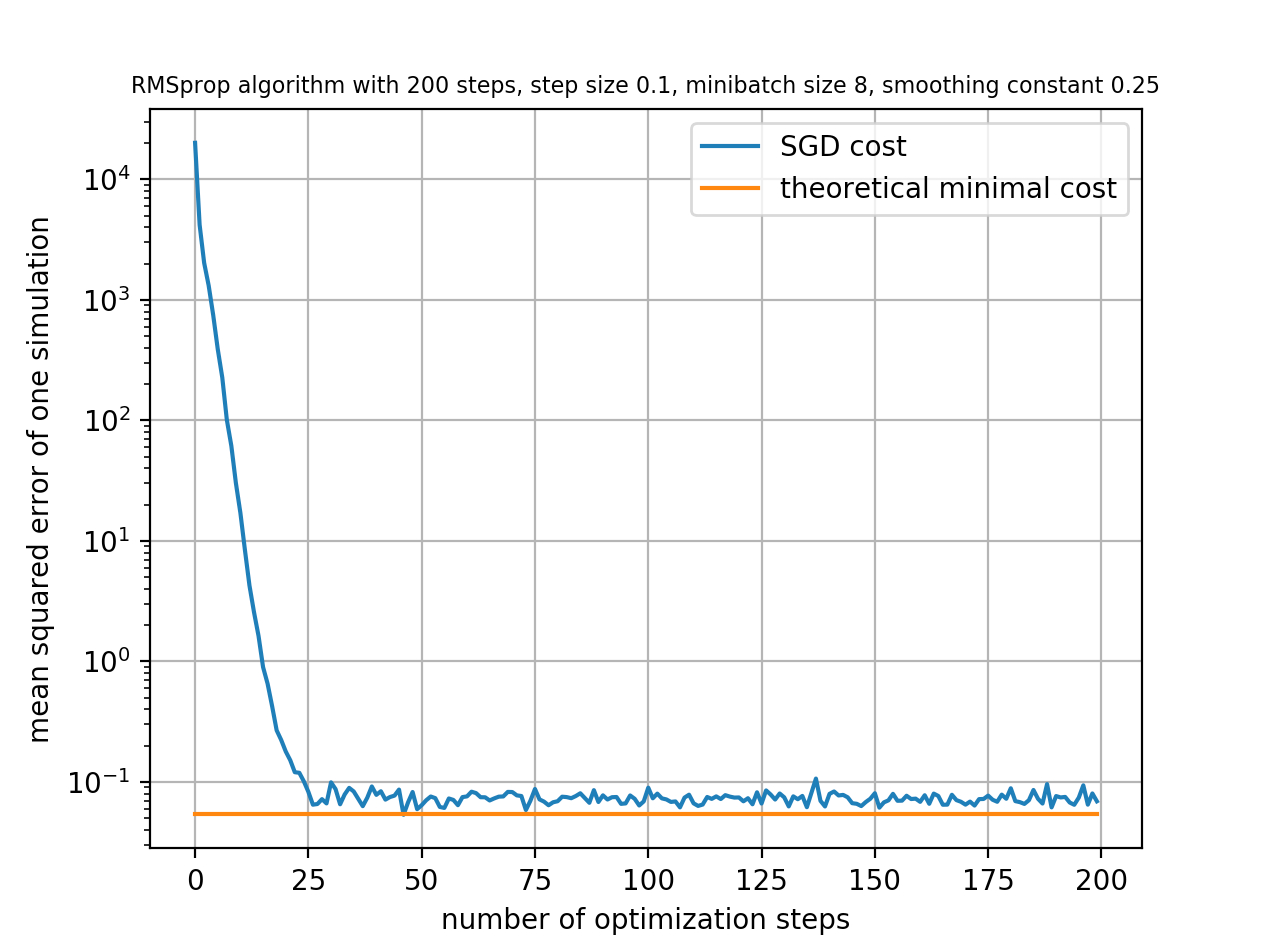
\includegraphics[width=1.0\textwidth]{Figures/beta_0_25.png}
		\caption{$\beta = 0.25$: cost w.r.t $n$}
	\end{minipage}%
	\begin{minipage}[t]{.28\paperwidth}
		\centering
		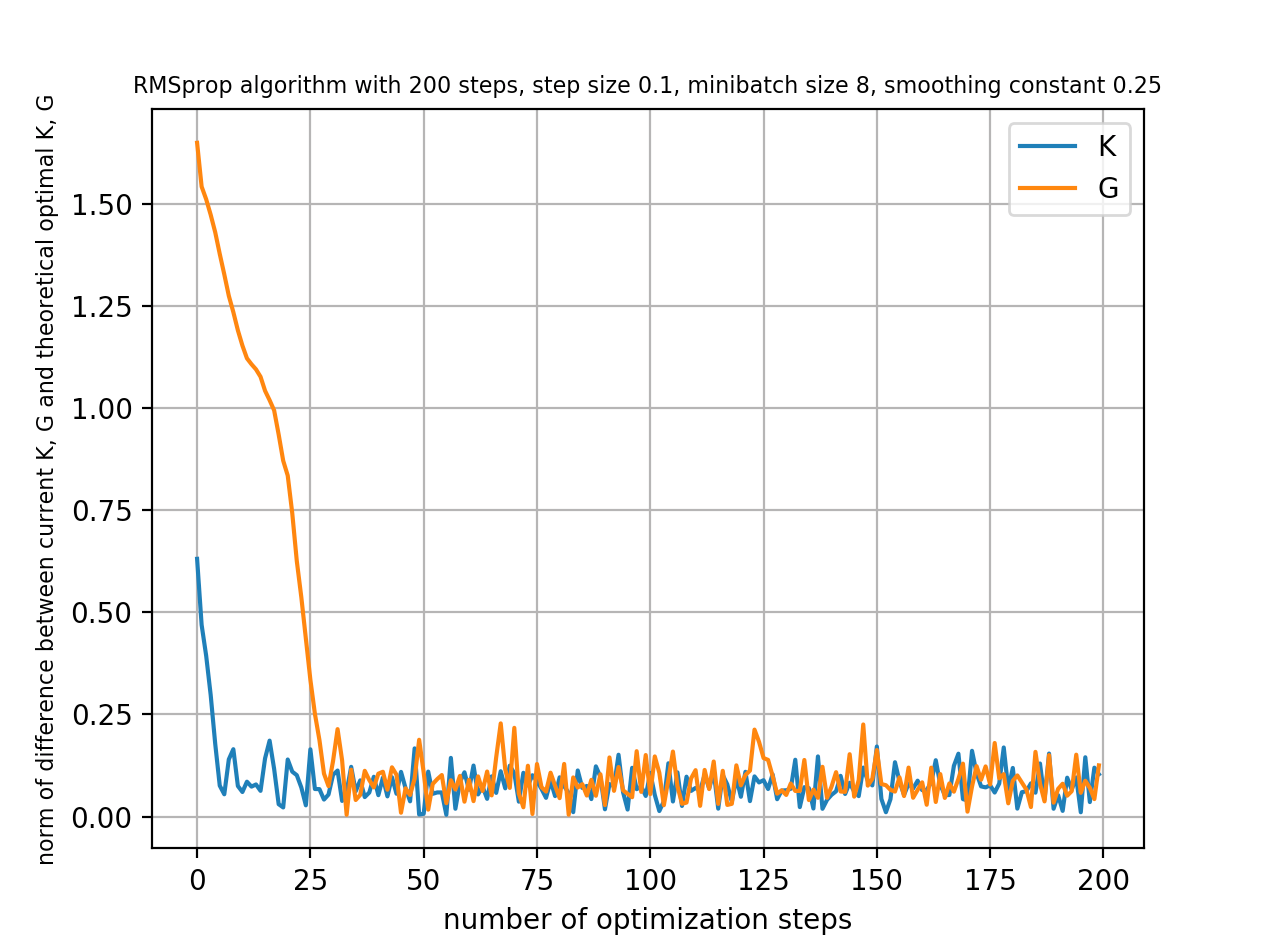
\includegraphics[width=1.0\textwidth]{Figures/d_beta_0_25.png}
		\caption{$\beta = 0.25$: difference between $K$, $G$ and theoretical steady state $K$, $G$ w.r.t $n$}
	\end{minipage}%
	\begin{minipage}[t]{.28\paperwidth}
		\centering
		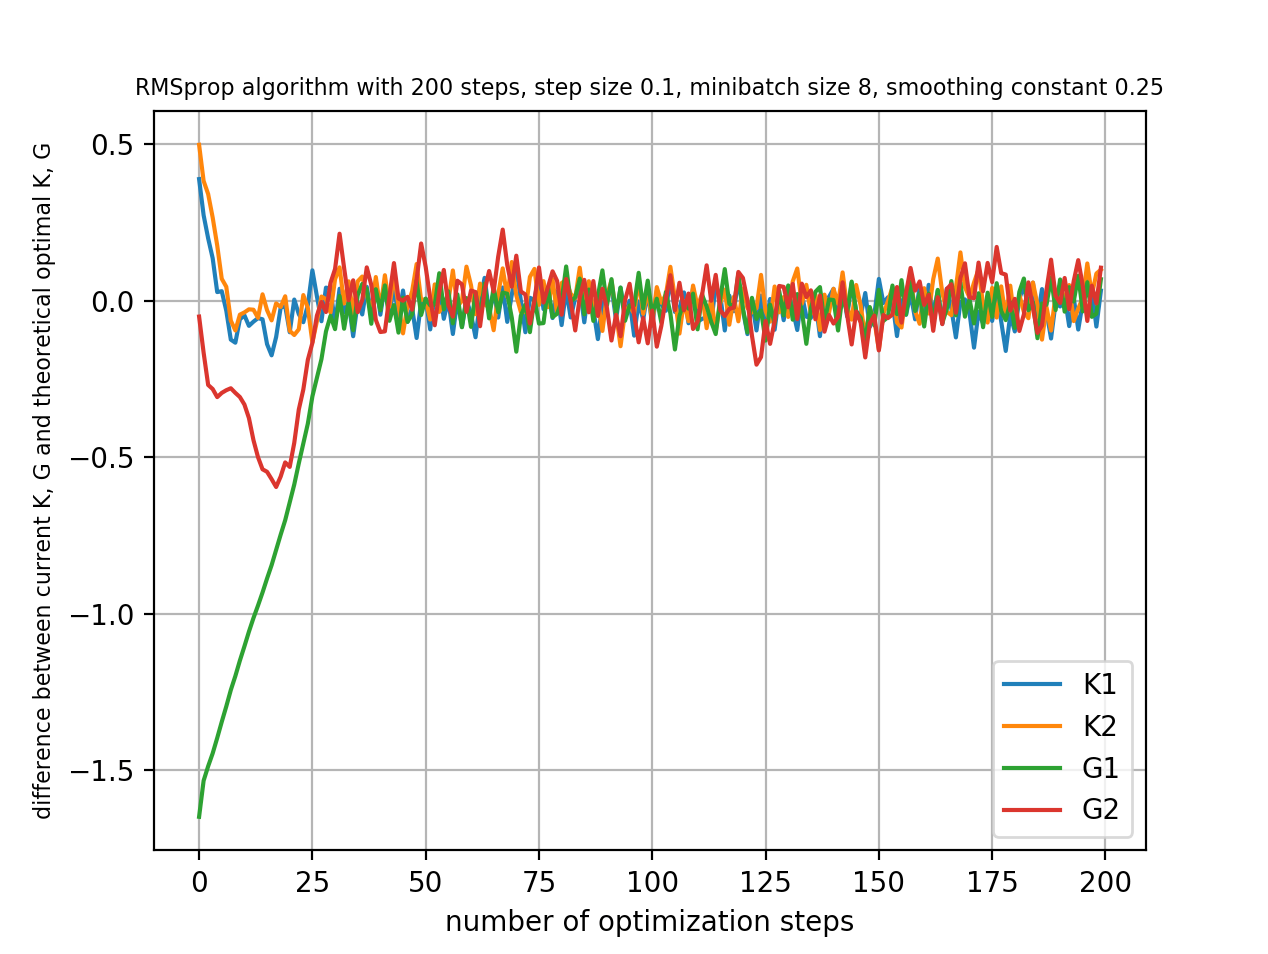
\includegraphics[width=1.0\textwidth]{Figures/d_beta_0_25_sep.png}
		\caption{$\beta = 0.25$: difference between $K$, $G$ and theoretical steady state $K$, $G$ w.r.t $n$ (element-wise) \label{fig:d_beta_0_25_sep}}
	\end{minipage}
\end{figure}
\begin{figure}[h!]
	\centering
	\begin{minipage}[t]{.28\paperwidth}
		\centering
		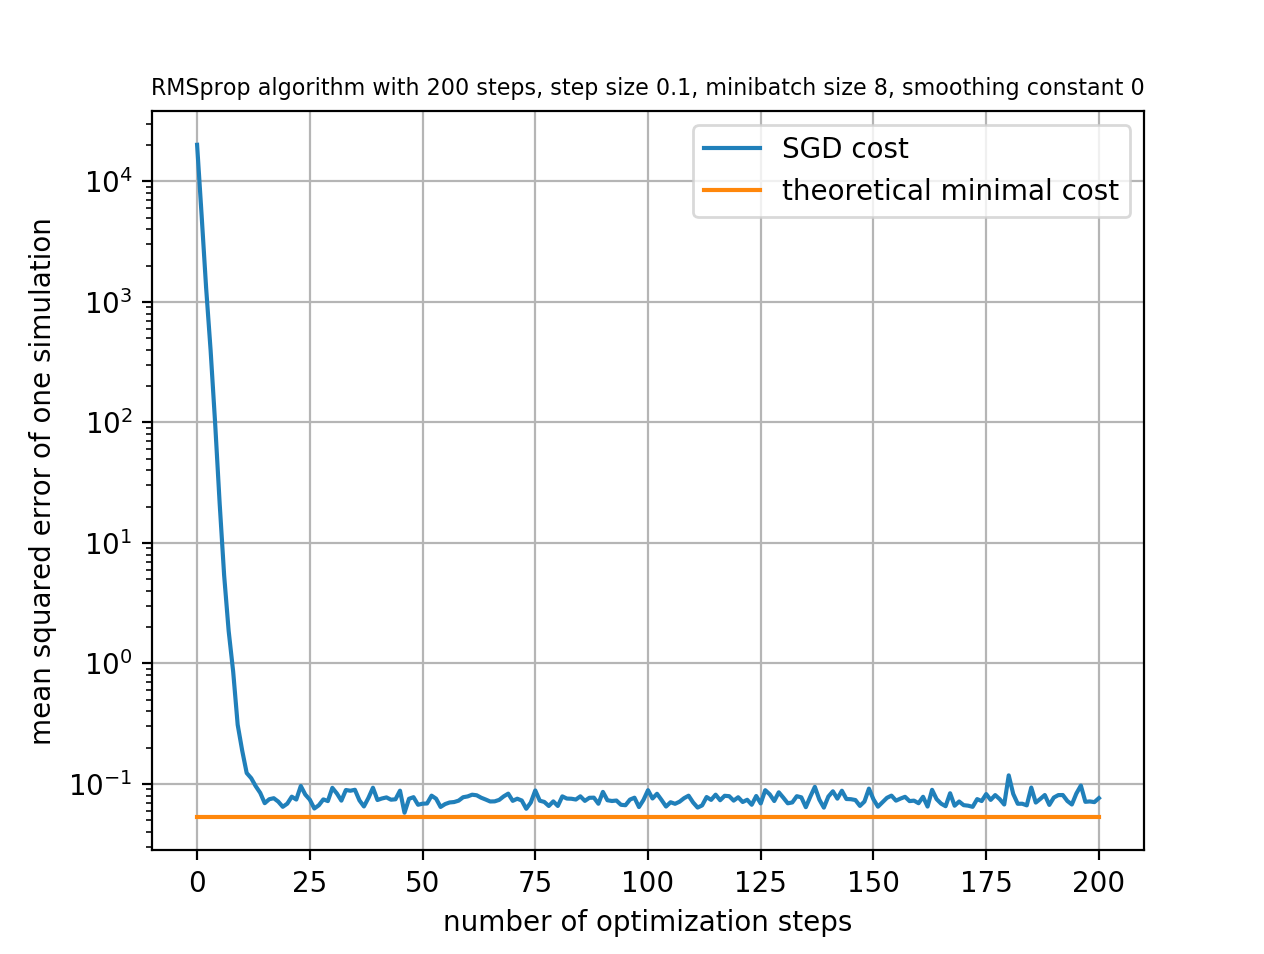
\includegraphics[width=1.0\textwidth]{Figures/beta_0.png}
		\caption{$\beta = 0.00$: cost w.r.t $n$}
	\end{minipage}%
	\begin{minipage}[t]{.28\paperwidth}
		\centering
		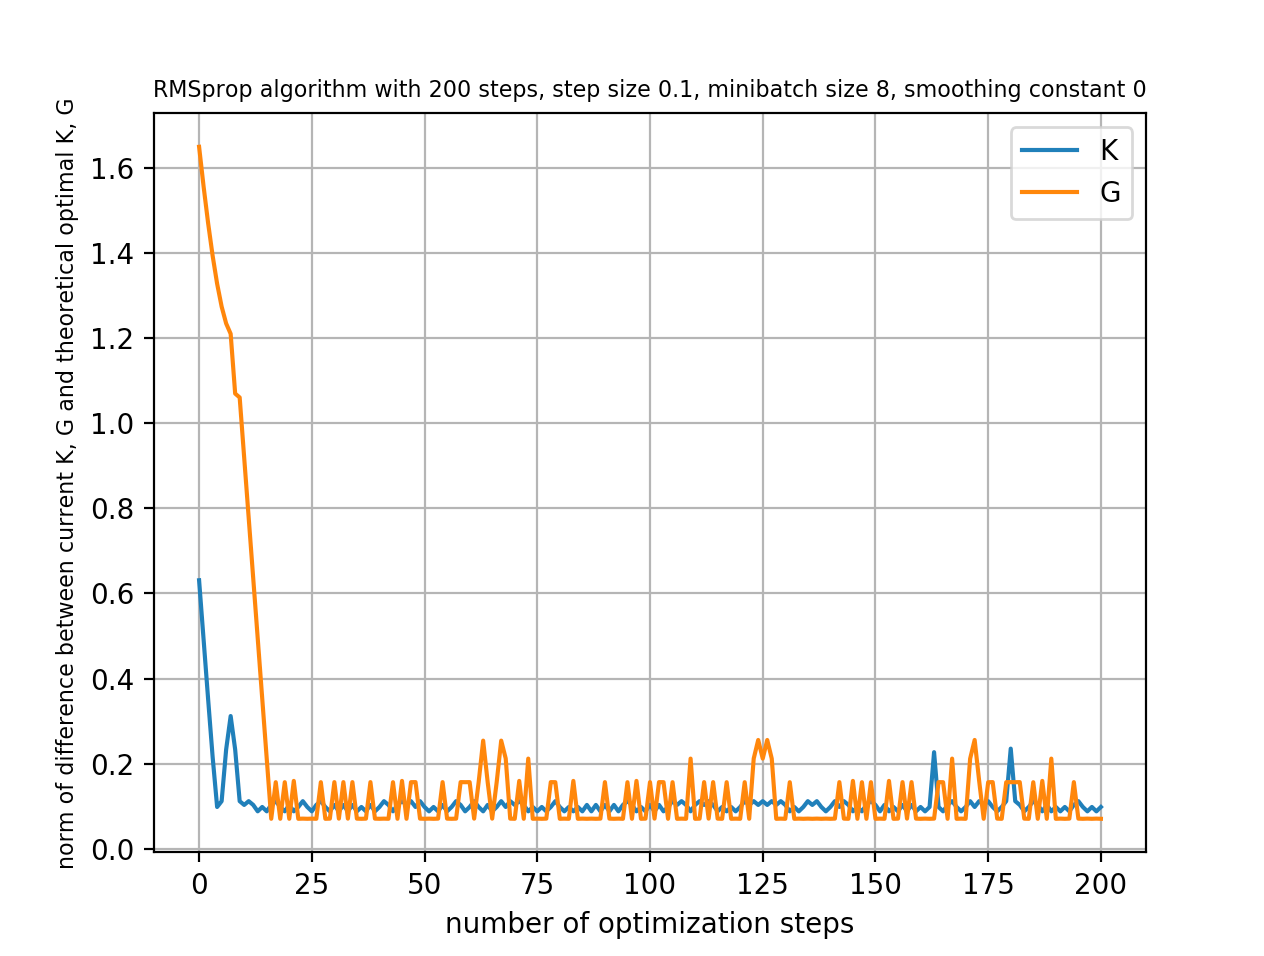
\includegraphics[width=1.0\textwidth]{Figures/d_beta_0.png}
		\caption{$\beta = 0.00$: difference between $K$, $G$ and theoretical steady state $K$, $G$ w.r.t $n$}
	\end{minipage}%
	\begin{minipage}[t]{.28\paperwidth}
		\centering
		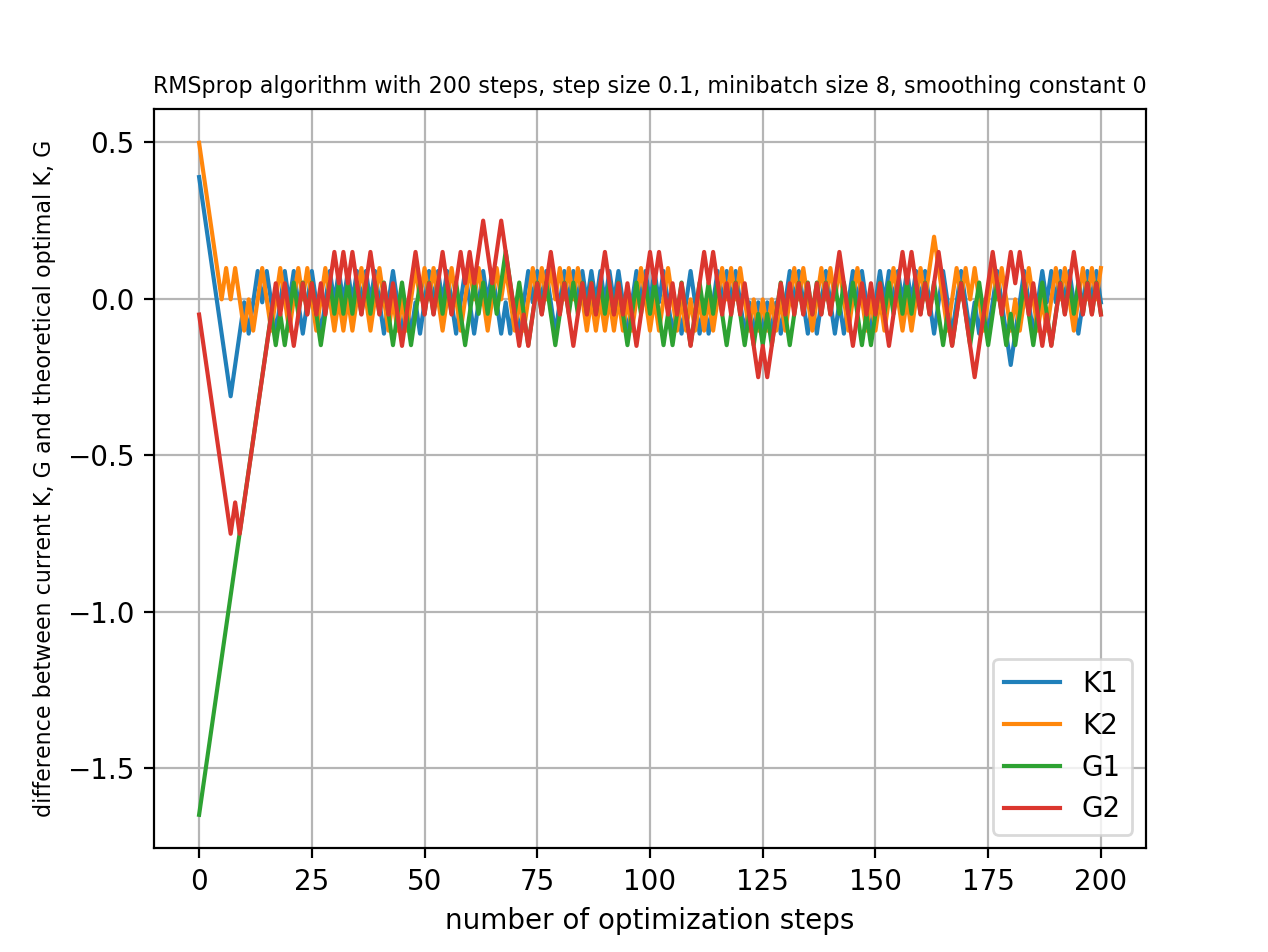
\includegraphics[width=1.0\textwidth]{Figures/d_beta_0_sep.png}
		\caption{$\beta = 0.00$: difference between $K$, $G$ and theoretical steady state $K$, $G$ w.r.t $n$ (element-wise) \label{fig:d_beta_0_sep}}
	\end{minipage}
\end{figure}
\begin{figure}[h!]
	\centering
	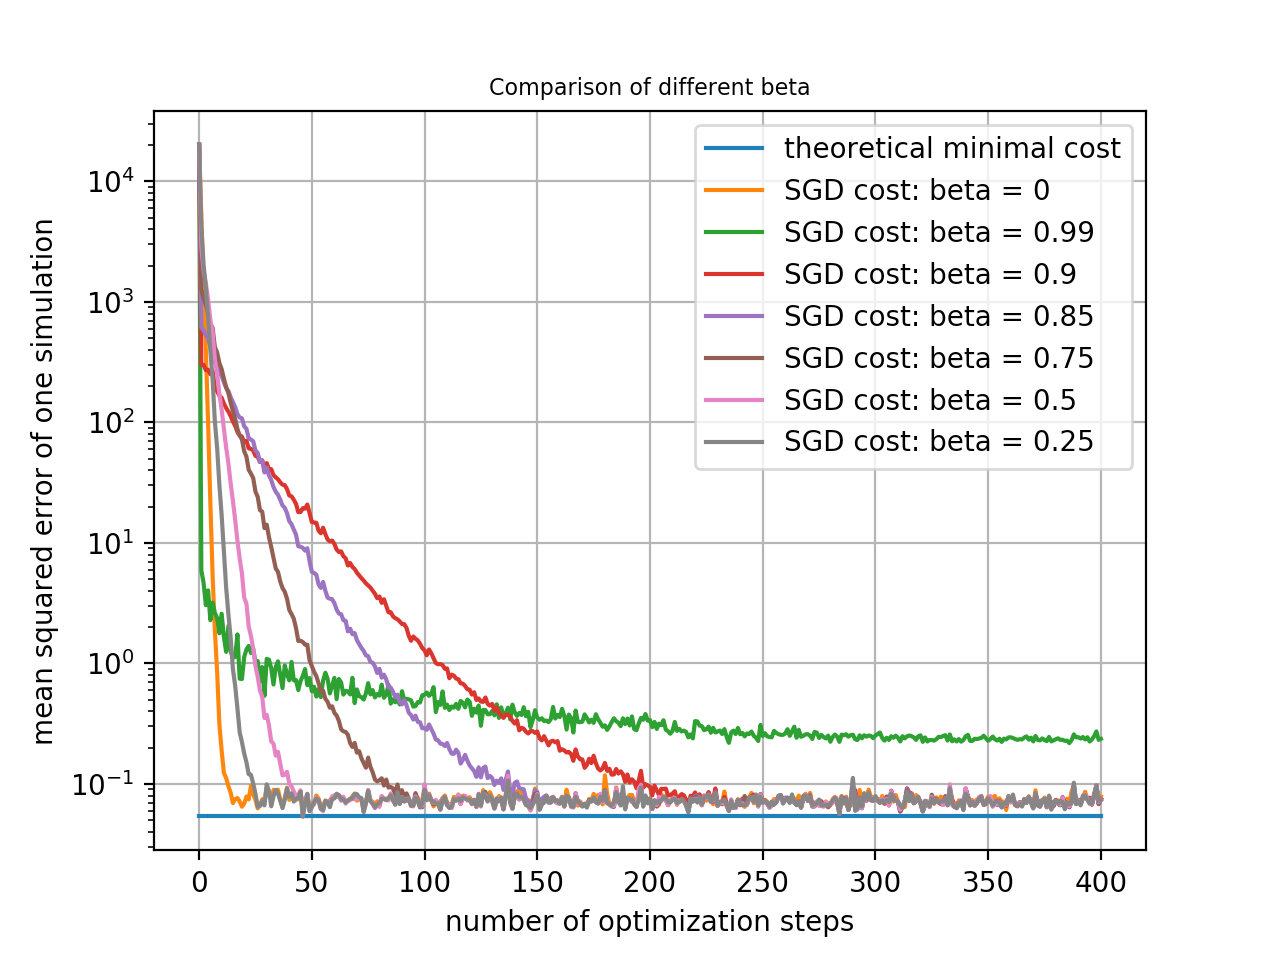
\includegraphics[width=0.5\textwidth]{Figures/comp_beta.png}
	\caption{Comparison of different $\beta$}
	\label{fig:comp_beta}
\end{figure}
\clearpage

\paragraph{Experiments with $M$}
Bearing a similar idea to the Sample Average Approximation algorithm, in the presence of the noise, mini-batch gradient descent is generally preferred over purely stochastic gradient descent in machine learning, as it is less prone to the noisiness of the samples. In our problem, we also investigate the influence of mini-batch sizes on the performance of the RMSprop algorithm through a series of experiments.

\noindent In the following experiments, $n = 400$ and $\beta = 0.9$. A comparison of the results is demonstrated in table \ref{table:1}. The first row in the table shows the theoretical result. Figures \ref{fig:M_1} to \ref{fig:d_M512_sep} plot the decay in the cost, the decay in the difference between $K$, $G$ and theoretical steady state $K$, $G$ in L2 norm, and the decay in the element-wise difference between $K$, $G$ and theoretical steady state $K$, $G$ w.r.t. $n$ for different $M$s. Figure \ref{fig:comp_M} offers a more intuitive comparison of the performances of different $M$s. From the results we can see that larger mini-batches can effectively reduce the noise in the gradient, as they produce smoother learning curves. However, whether increasing mini-batch size can improve numerical accuracy is not very clear. By comparing the results, it seems that $M = 8$ is able to achieve both relatively good accuracy as well as data efficiency.\\
\begin{table}[h!]
	\begin{center}
		\begin{tabular}{|c|m{3.3cm}|c|m{1.7cm}|m{1.7cm}|c|c|} 
			\hline
			$M$ & ultimate $K$ & ultimate $G$ & final $K$ difference & final $G$ difference & final cost & testing cost \\ 
			\hline
			- & $\begin{bmatrix}1.12\times 10^{-1} \\ 2.44\times 10^{-3}\end{bmatrix}$ & $[6.49\times 10^{-1}, -4.89\times 10^{-2}]$ & -- & -- & -- & $5.37\times 10^{-2}$\\
			\hline
			\hline
			1 & $\begin{bmatrix}2.57\times 10^{-1} \\ -1.34\times 10^{-1}\end{bmatrix}$ & $[6.01\times 10^{-1}, 1.69\times 10^{-3}]$ & $1.99\times 10^{-1}$ & $6.94\times 10^{-2}$ & $6.59\times 10^{-2}$ & $8.12\times 10^{-2}$\\ 
			\hline
			8 & $\begin{bmatrix}1.13\times 10^{-1} \\ 1.91\times 10^{-2}\end{bmatrix}$ & $[6.11\times 10^{-1}, -1.28\times 10^{-1}]$ & $1.67\times 10^{-2}$ & $8.81\times 10^{-2}$ & $7.45\times 10^{-2}$ & $7.01\times 10^{-2}$\\ 
			\hline
			16 & $\begin{bmatrix}8.80\times 10^{-2} \\ 2.72\times 10^{-2}\end{bmatrix}$ & $[6.58\times 10^{-1}, 8.83\times 10^{-3}]$ & $3.44\times 10^{-2}$ & $5.84\times 10^{-2}$ & $6.80\times 10^{-2}$ & $7.15\times 10^{-2}$\\ 
			\hline
			32 & $\begin{bmatrix}9.23\times 10^{-2} \\ 2.69\times 10^{-2}\end{bmatrix}$ & $[6.19\times 10^{-1}, 2.01\times 10^{-2}]$ & $3.14\times 10^{-2}$ & $7.52\times 10^{-2}$ & $6.68\times 10^{-2}$ & $7.05\times 10^{-2}$\\ 
			\hline
			64 & $\begin{bmatrix}9.92\times 10^{-2} \\ 4.59\times 10^{-2}\end{bmatrix}$ & $[6.55\times 10^{-1}, -7.56\times 10^{-2}]$ & $4.53\times 10^{-2}$ & $2.75\times 10^{-2}$ & $6.80\times 10^{-2}$ & $6.98\times 10^{-2}$\\
			\hline
			128 & $\begin{bmatrix}3.48\times 10^{-2} \\ 3.71\times 10^{-3}\end{bmatrix}$ & $[5.20\times 10^{-1}, -9.11\times 10^{-2}]$ & $7.72\times 10^{-2}$ & $1.36\times 10^{-1}$ & $7.39\times 10^{-2}$ & $7.30\times 10^{-2}$\\ 
			\hline
			256 & $\begin{bmatrix}2.10\times 10^{-1} \\ -4.35\times 10^{-3}\end{bmatrix}$ & $[7.19\times 10^{-1}, 3.44\times 10^{-2}]$ & $9.83\times 10^{-2}$ & $1.09\times 10^{-1}$ & $7.73\times 10^{-2}$ & $7.71\times 10^{-2}$\\ 
			\hline
			512 & $\begin{bmatrix}2.74\times 10^{-2} \\ -1.80\times 10^{-2}\end{bmatrix}$ & $[5.73\times 10^{-1}, -6.26\times 10^{-2}]$ & $8.70\times 10^{-2}$ & $7.66\times 10^{-2}$ & $7.33\times 10^{-2}$ & $7.26\times 10^{-2}$\\ 
			\hline
		\end{tabular}
	\end{center}
	\caption{Comparison of different mini-batch sizes}
	\label{table:1}
\end{table}
\begin{figure}[h!]
	\centering
	\begin{minipage}[t]{.28\paperwidth}
		\centering
		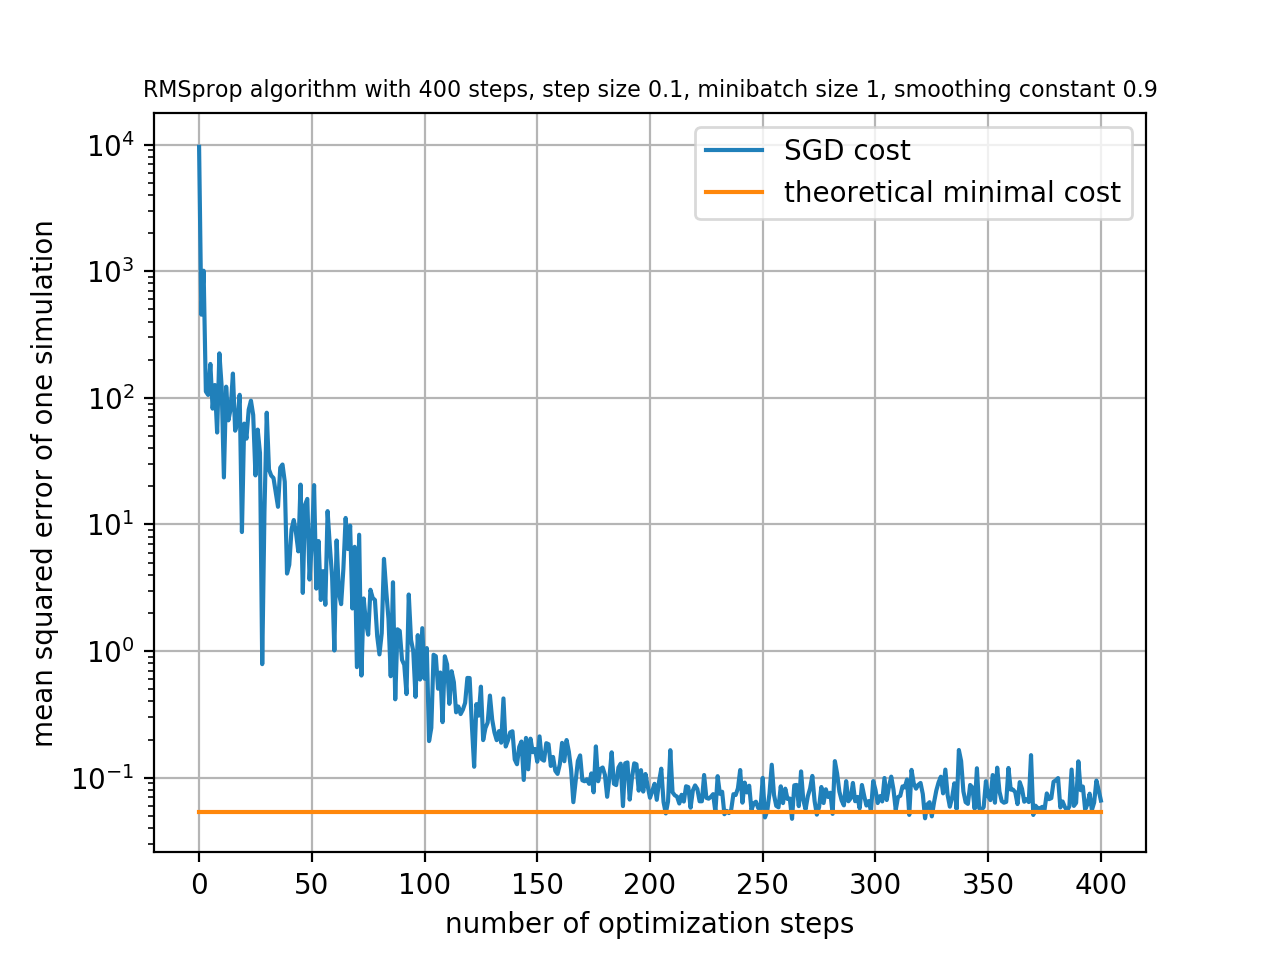
\includegraphics[width=1.0\textwidth]{Figures/M1.png}
		\caption{$M=1$: cost w.r.t $n$ \label{fig:M_1}}
	\end{minipage}%
	\begin{minipage}[t]{.28\paperwidth}
		\centering
		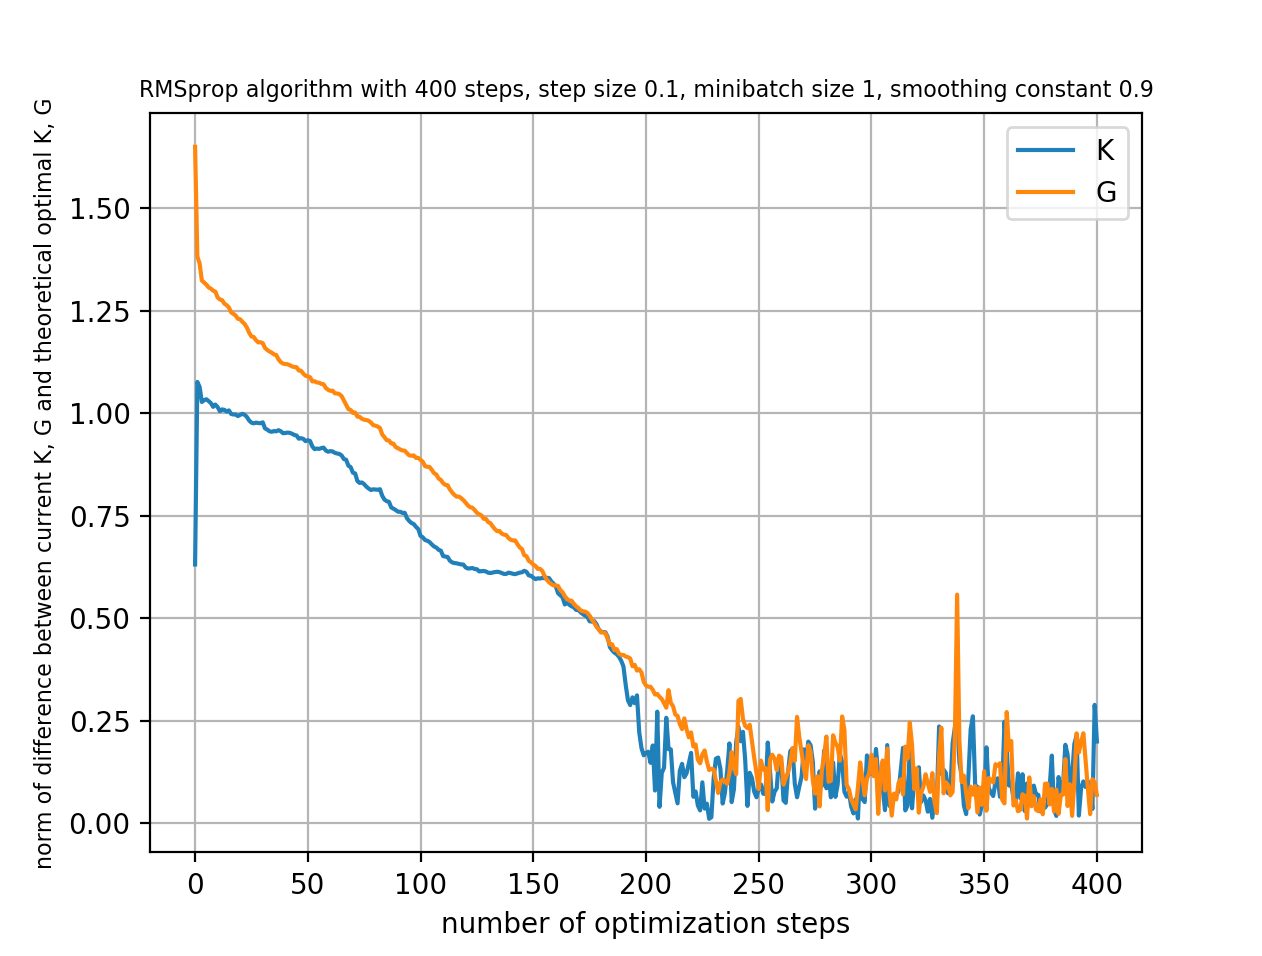
\includegraphics[width=1.0\textwidth]{Figures/d_M1.png}
		\caption{$M=1$: difference between $K$, $G$ and theoretical steady state $K$, $G$ w.r.t $n$}
	\end{minipage}%
	\begin{minipage}[t]{.28\paperwidth}
		\centering
		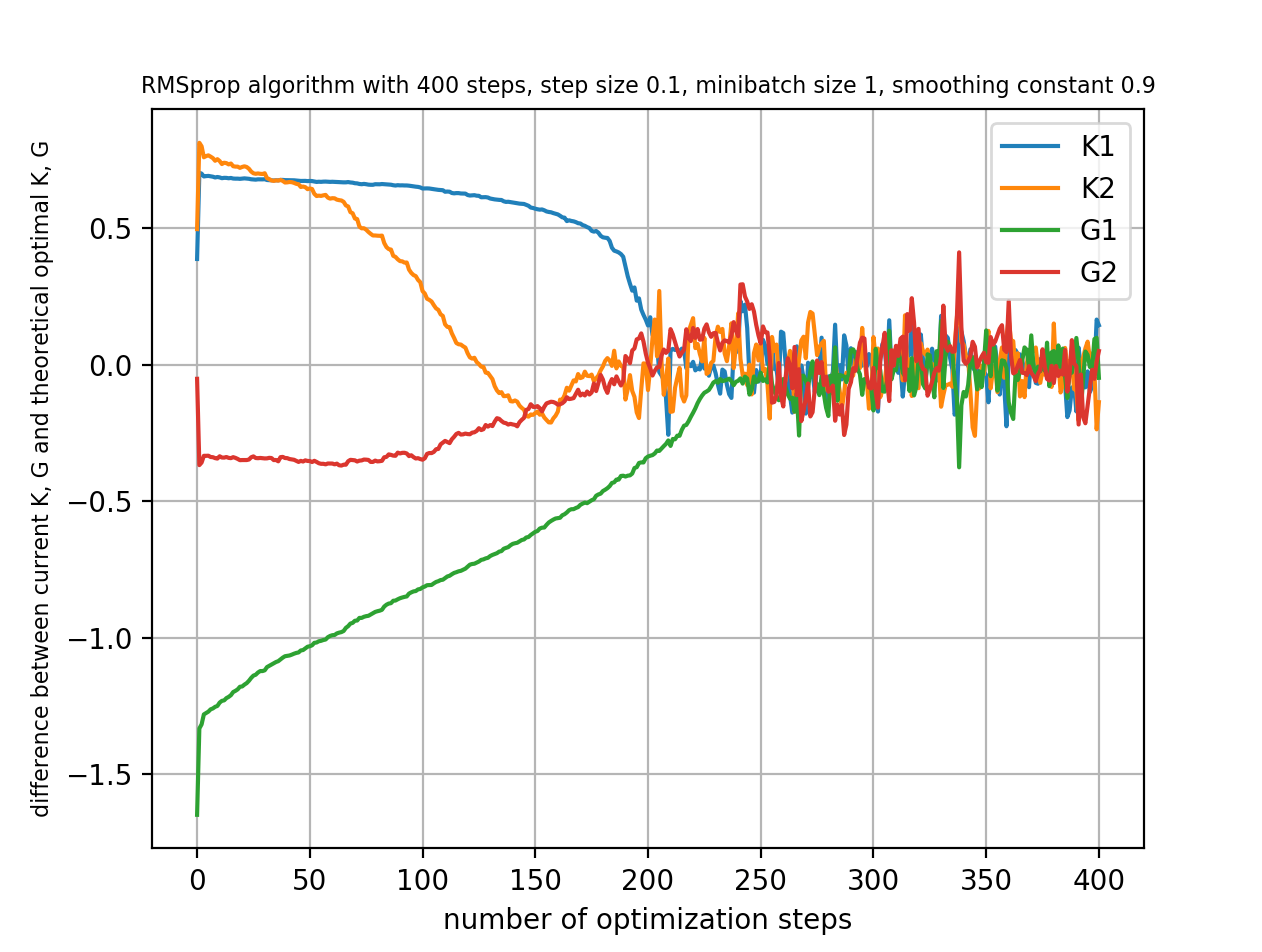
\includegraphics[width=1.0\textwidth]{Figures/d_M1_sep.png}
		\caption{$M=1$: difference between $K$, $G$ and theoretical steady state $K$, $G$ w.r.t $n$ (element-wise)}
	\end{minipage}
\end{figure}
\begin{figure}[h!]
	\centering
	\begin{minipage}[t]{.28\paperwidth}
		\centering
		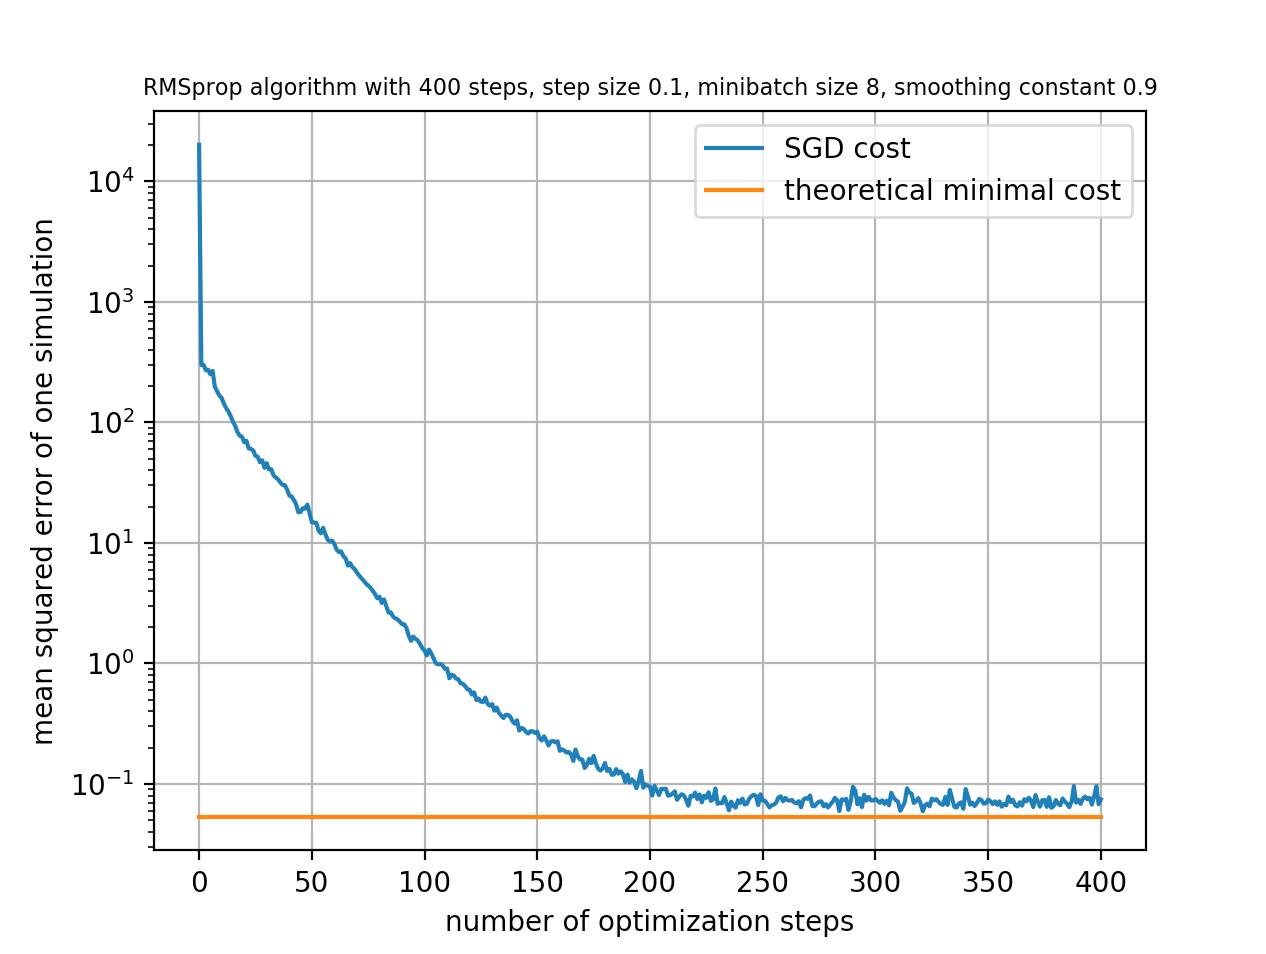
\includegraphics[width=1.0\textwidth]{Figures/M8.png}
		\caption{$M=8$: cost w.r.t $n$}
	\end{minipage}%
	\begin{minipage}[t]{.28\paperwidth}
		\centering
		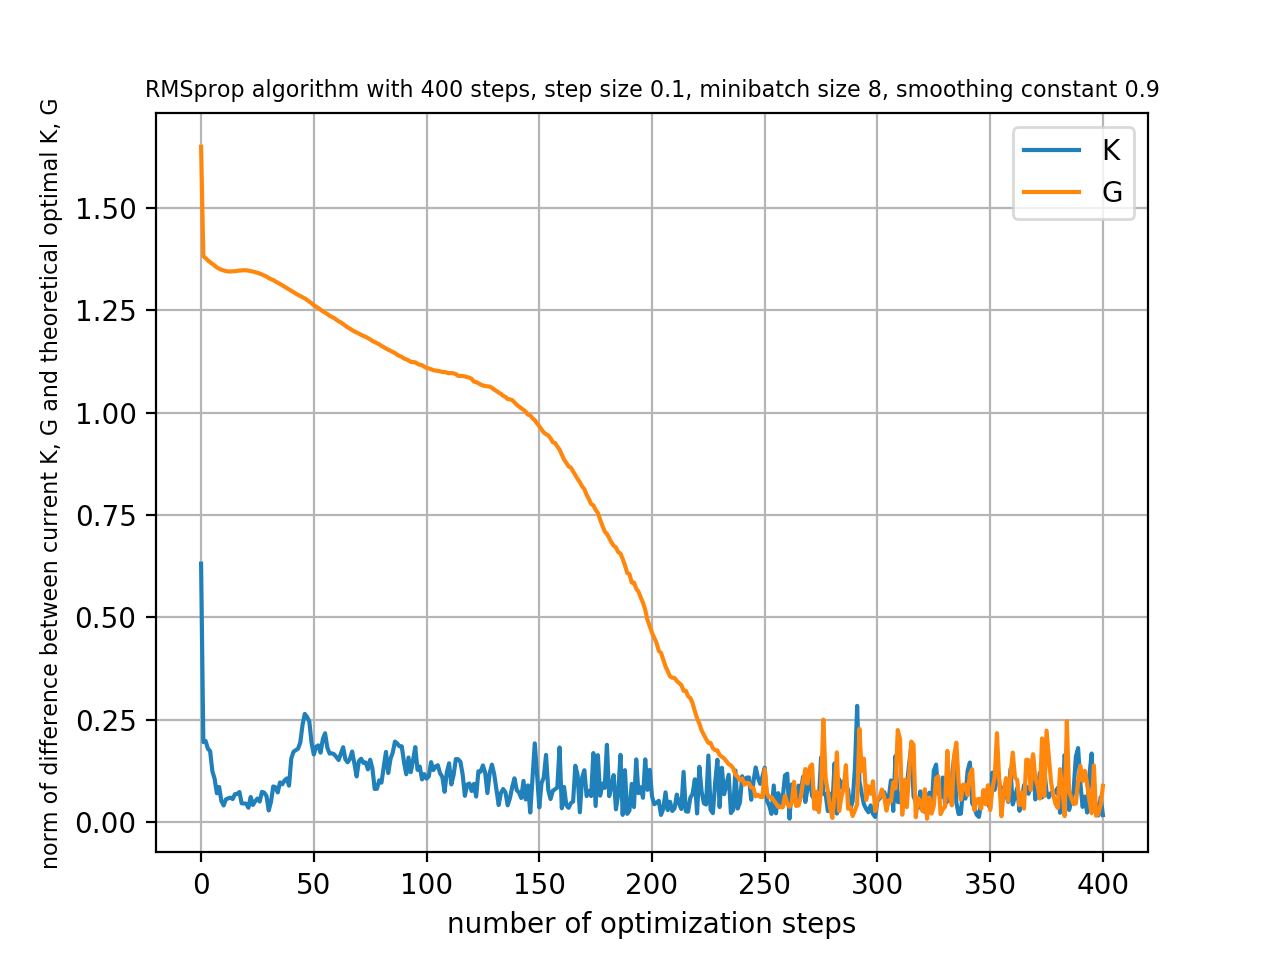
\includegraphics[width=1.0\textwidth]{Figures/d_M8.png}
		\caption{$M=8$: difference between $K$, $G$ and theoretical steady state $K$, $G$ w.r.t $n$}
	\end{minipage}%
	\begin{minipage}[t]{.28\paperwidth}
		\centering
		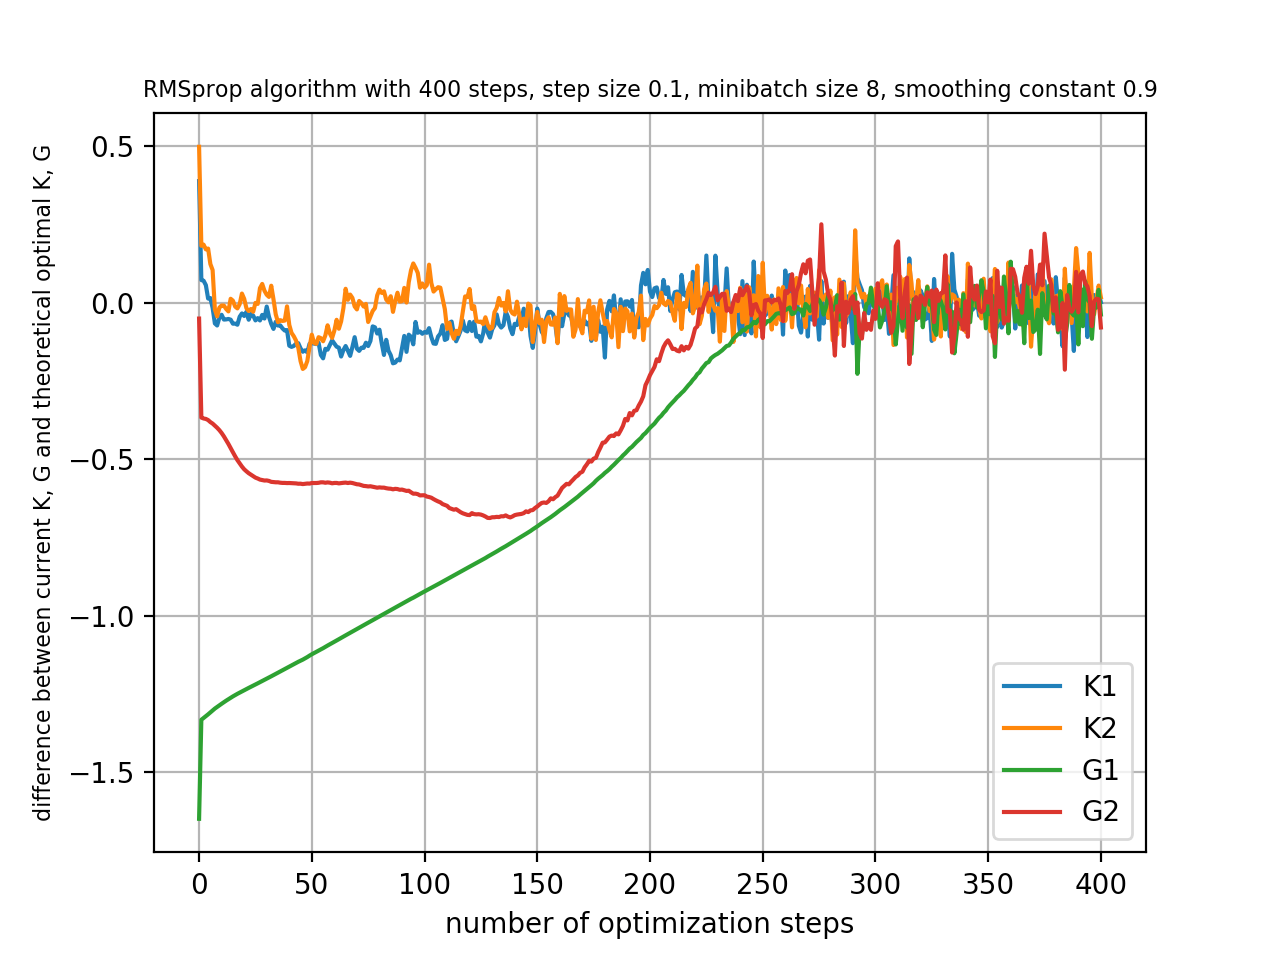
\includegraphics[width=1.0\textwidth]{Figures/d_M8_sep.png}
		\caption{$M=8$: difference between $K$, $G$ and theoretical steady state $K$, $G$ w.r.t $n$ (element-wise)}
	\end{minipage}
\end{figure}
\begin{figure}[h!]
	\centering
	\begin{minipage}[t]{.28\paperwidth}
		\centering
		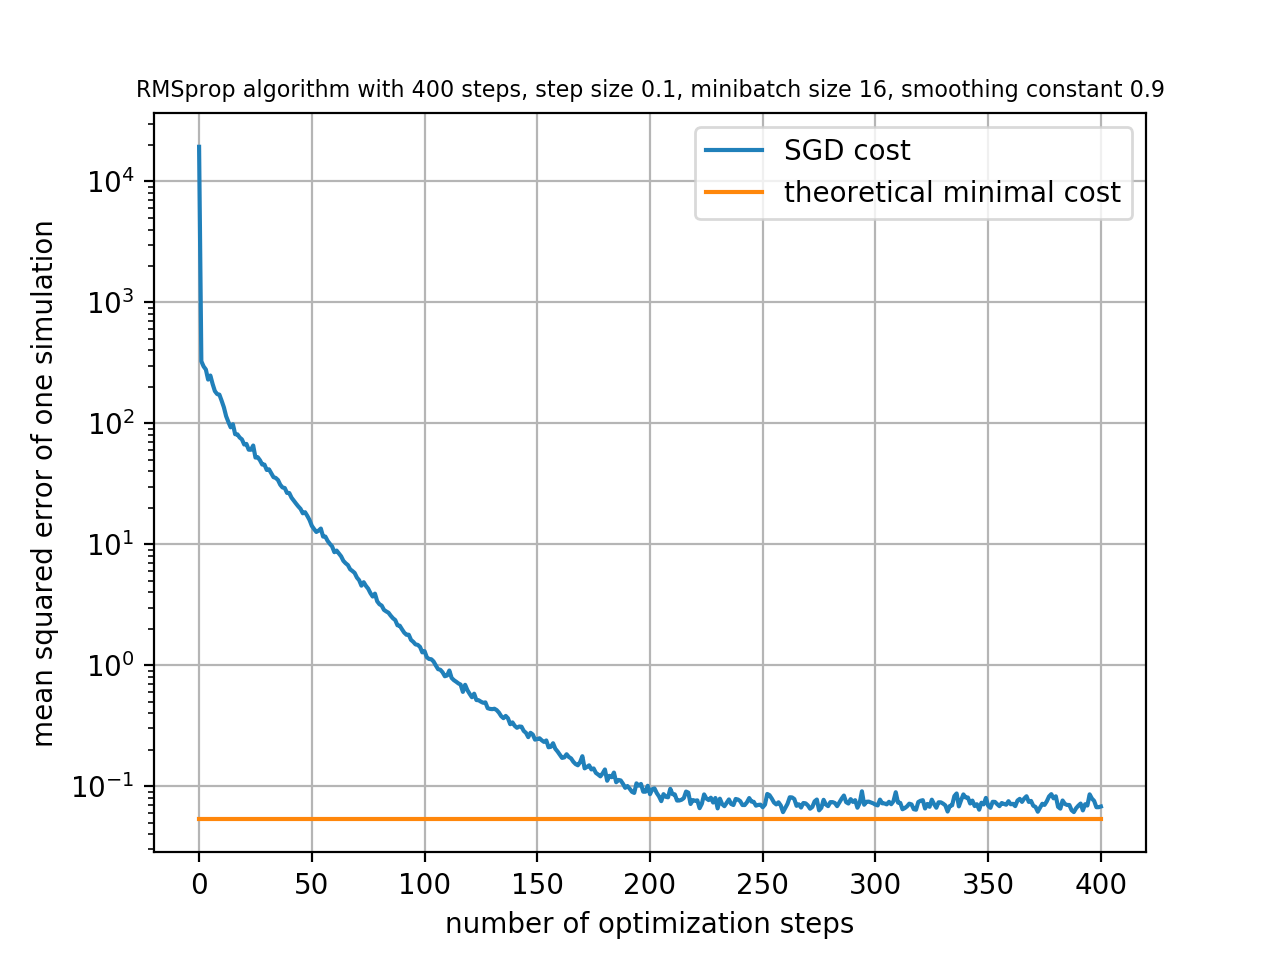
\includegraphics[width=1.0\textwidth]{Figures/M16.png}
		\caption{$M=16$: cost w.r.t $n$}
	\end{minipage}%
	\begin{minipage}[t]{.28\paperwidth}
		\centering
		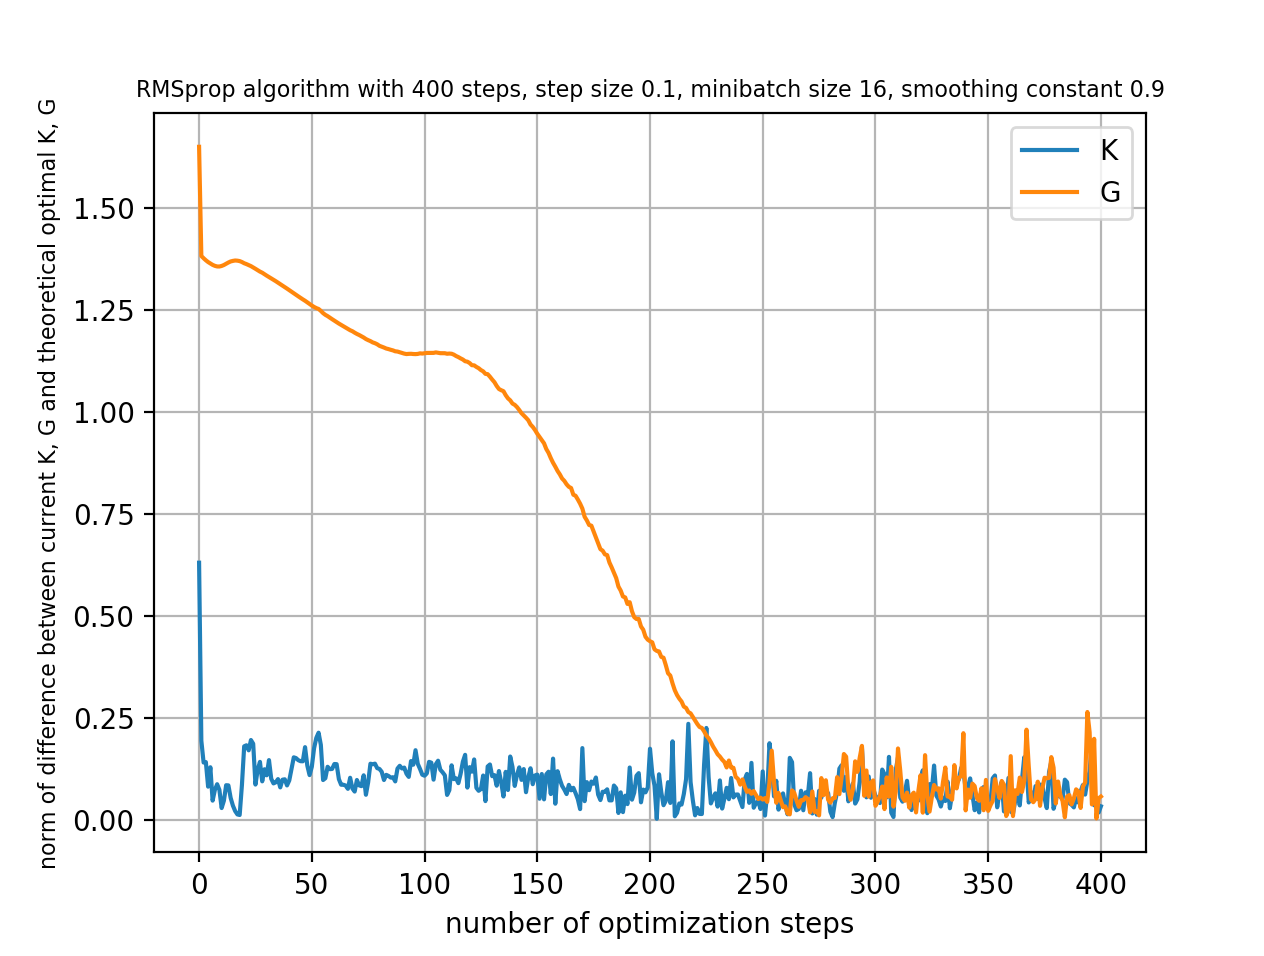
\includegraphics[width=1.0\textwidth]{Figures/d_M16.png}
		\caption{$M=16$: difference between $K$, $G$ and theoretical steady state $K$, $G$ w.r.t $n$}
	\end{minipage}%
	\begin{minipage}[t]{.28\paperwidth}
		\centering
		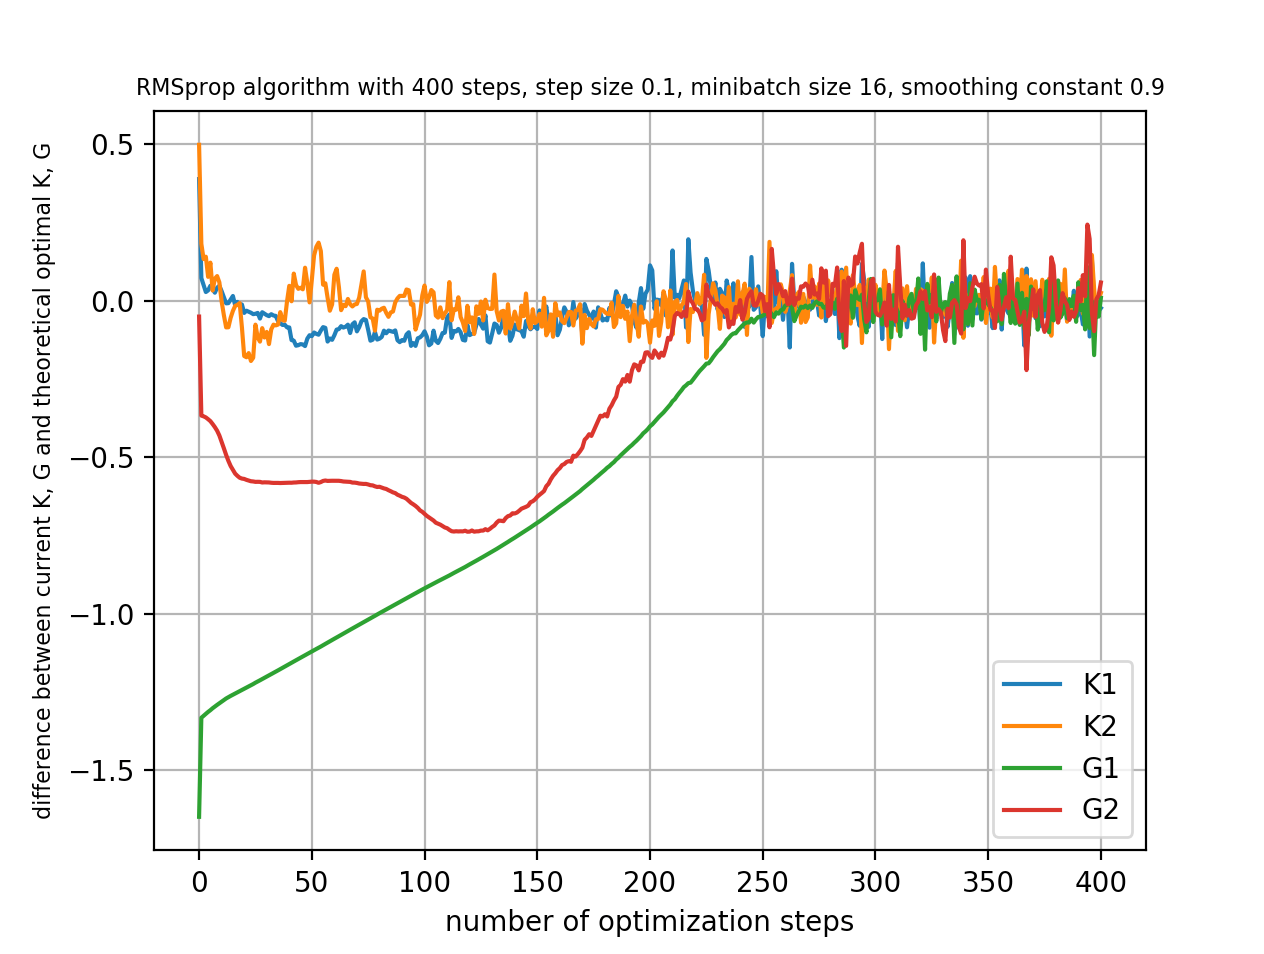
\includegraphics[width=1.0\textwidth]{Figures/d_M16_sep.png}
		\caption{$M=16$: difference between $K$, $G$ and theoretical steady state $K$, $G$ w.r.t $n$ (element-wise)}
	\end{minipage}
\end{figure}
\clearpage
\begin{figure}[h!]
	\centering
	\begin{minipage}[t]{.28\paperwidth}
		\centering
		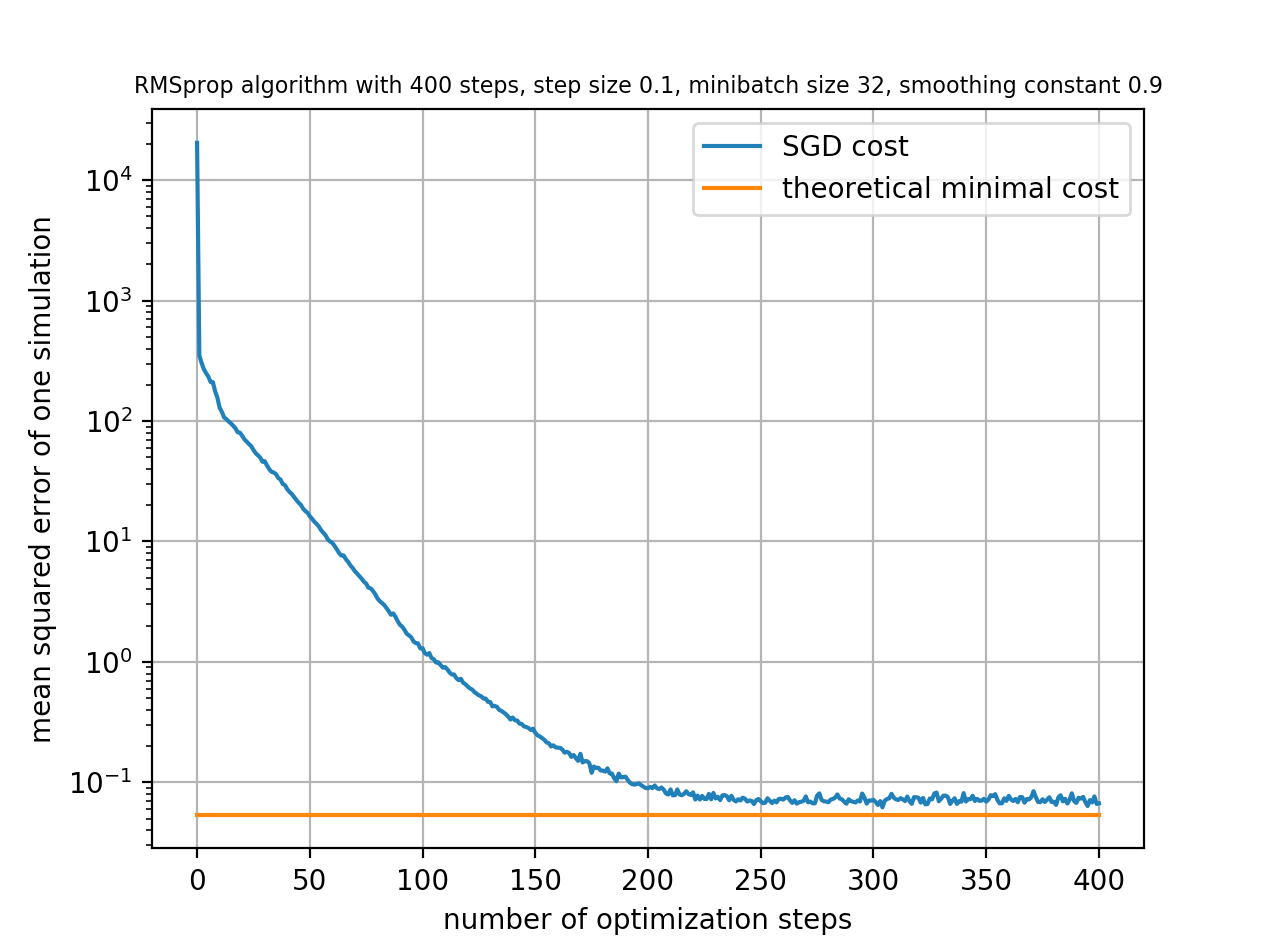
\includegraphics[width=1.0\textwidth]{Figures/M32.png}
		\caption{$M=32$: cost w.r.t $n$}
	\end{minipage}%
	\begin{minipage}[t]{.28\paperwidth}
		\centering
		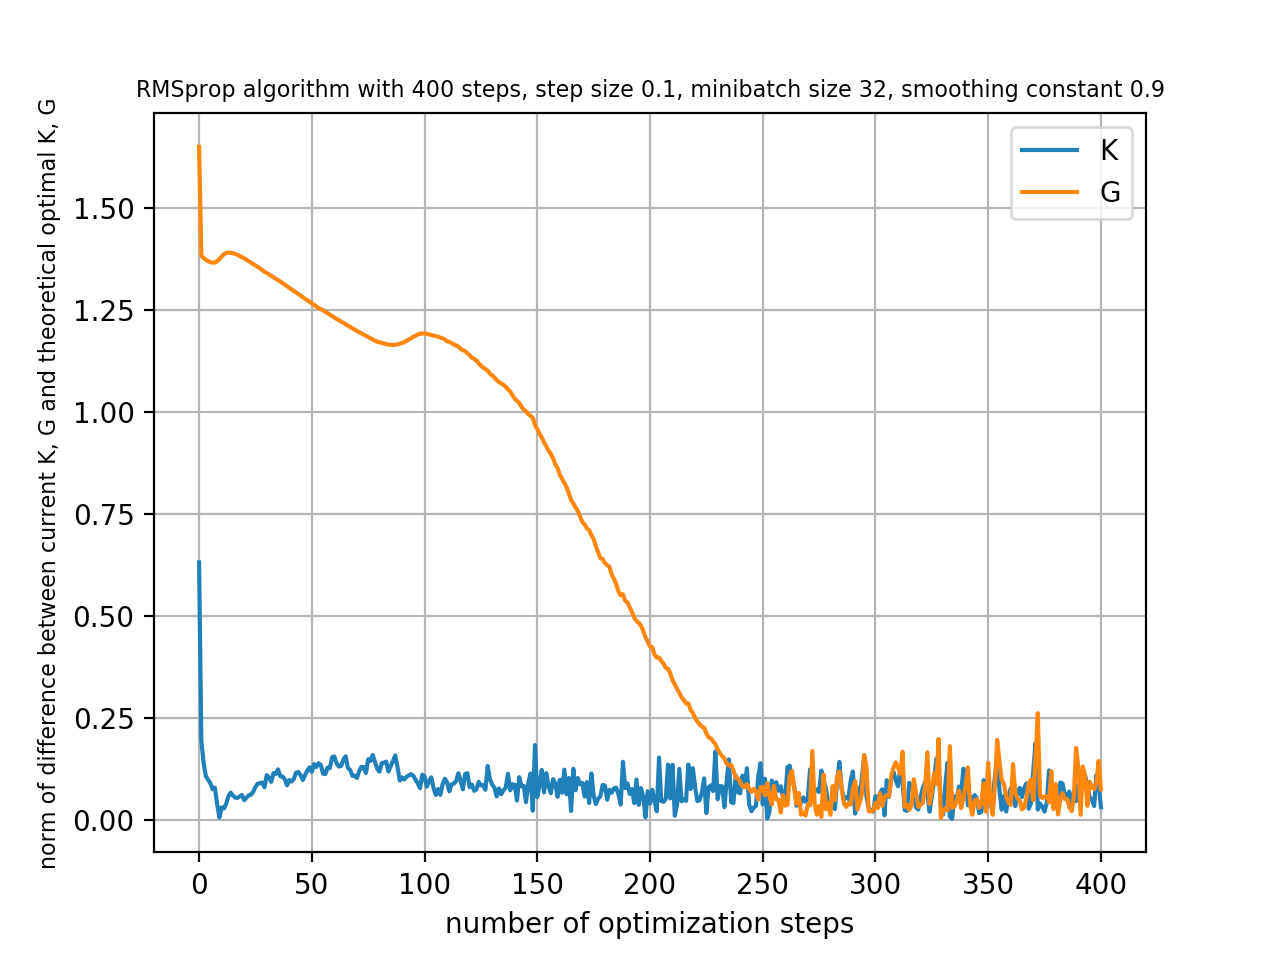
\includegraphics[width=1.0\textwidth]{Figures/d_M32.png}
		\caption{$M=32$: difference between $K$, $G$ and theoretical steady state $K$, $G$ w.r.t $n$}
	\end{minipage}%
	\begin{minipage}[t]{.28\paperwidth}
		\centering
		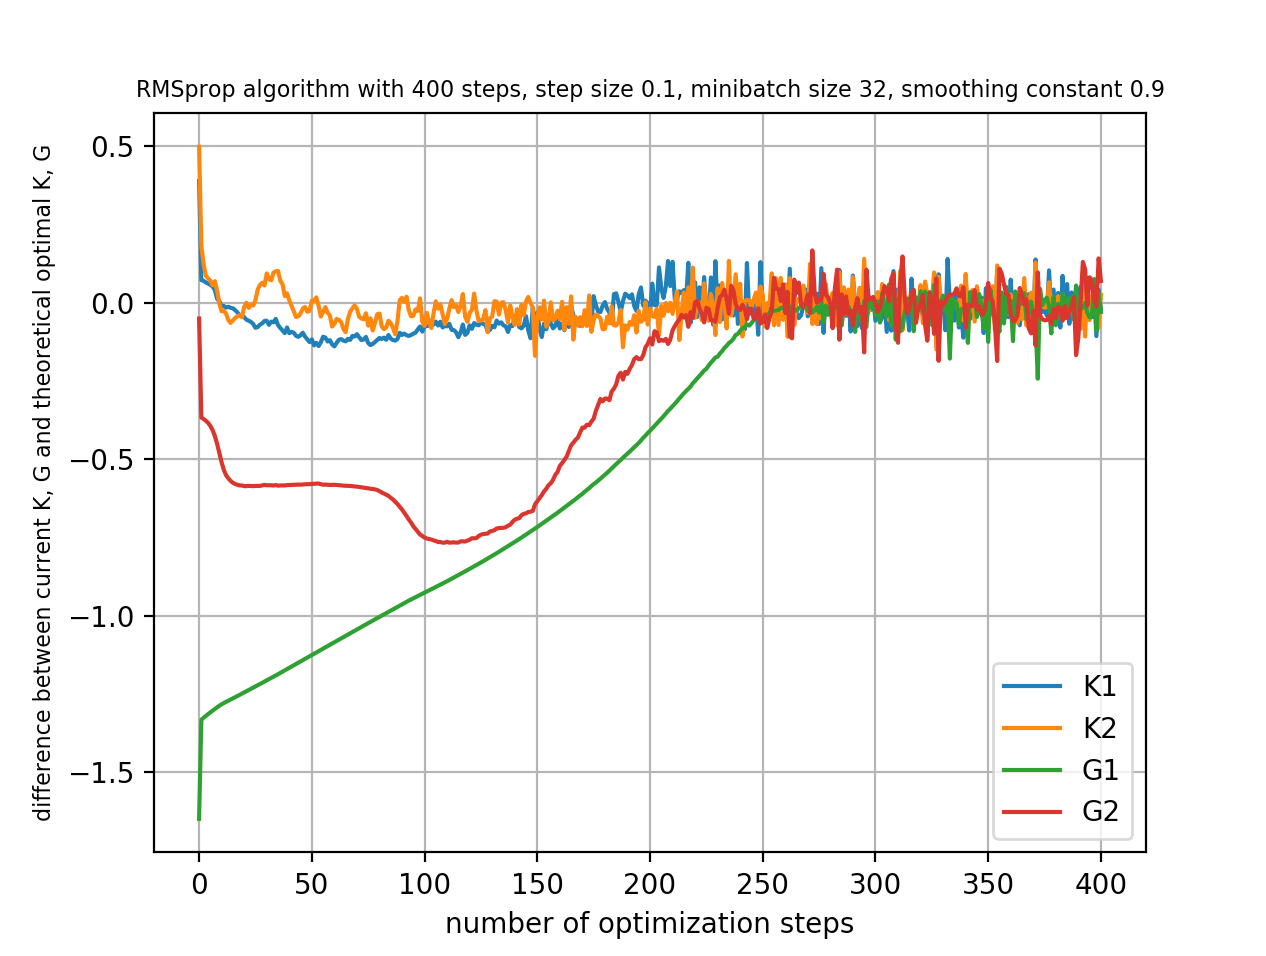
\includegraphics[width=1.0\textwidth]{Figures/d_M32_sep.png}
		\caption{$M=32$: difference between $K$, $G$ and theoretical steady state $K$, $G$ w.r.t $n$ (element-wise)}
	\end{minipage}
\end{figure}
\begin{figure}[h!]
	\centering
	\begin{minipage}[t]{.28\paperwidth}
		\centering
		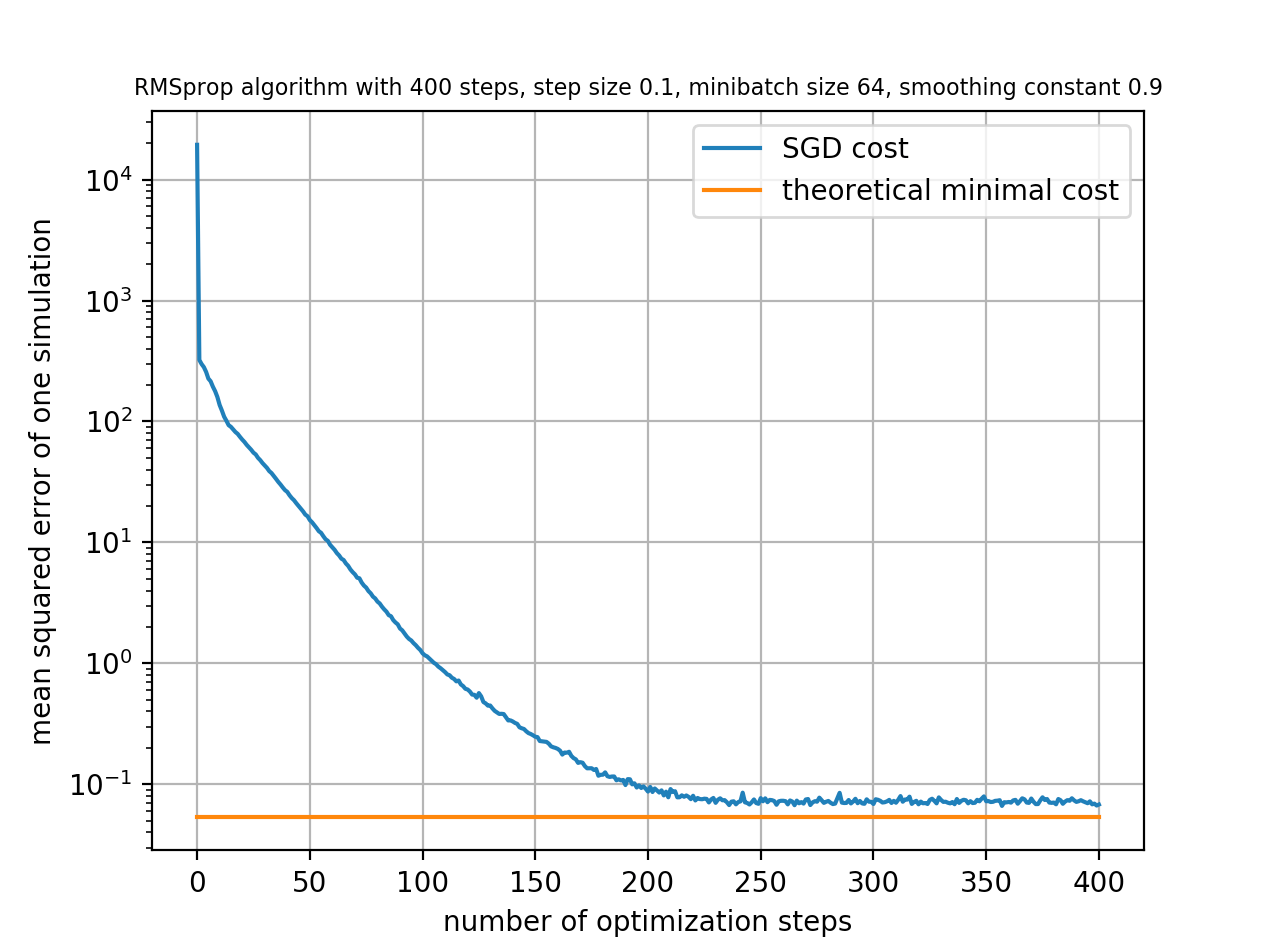
\includegraphics[width=1.0\textwidth]{Figures/M64.png}
		\caption{$M=64$: cost w.r.t $n$}
	\end{minipage}%
	\begin{minipage}[t]{.28\paperwidth}
		\centering
		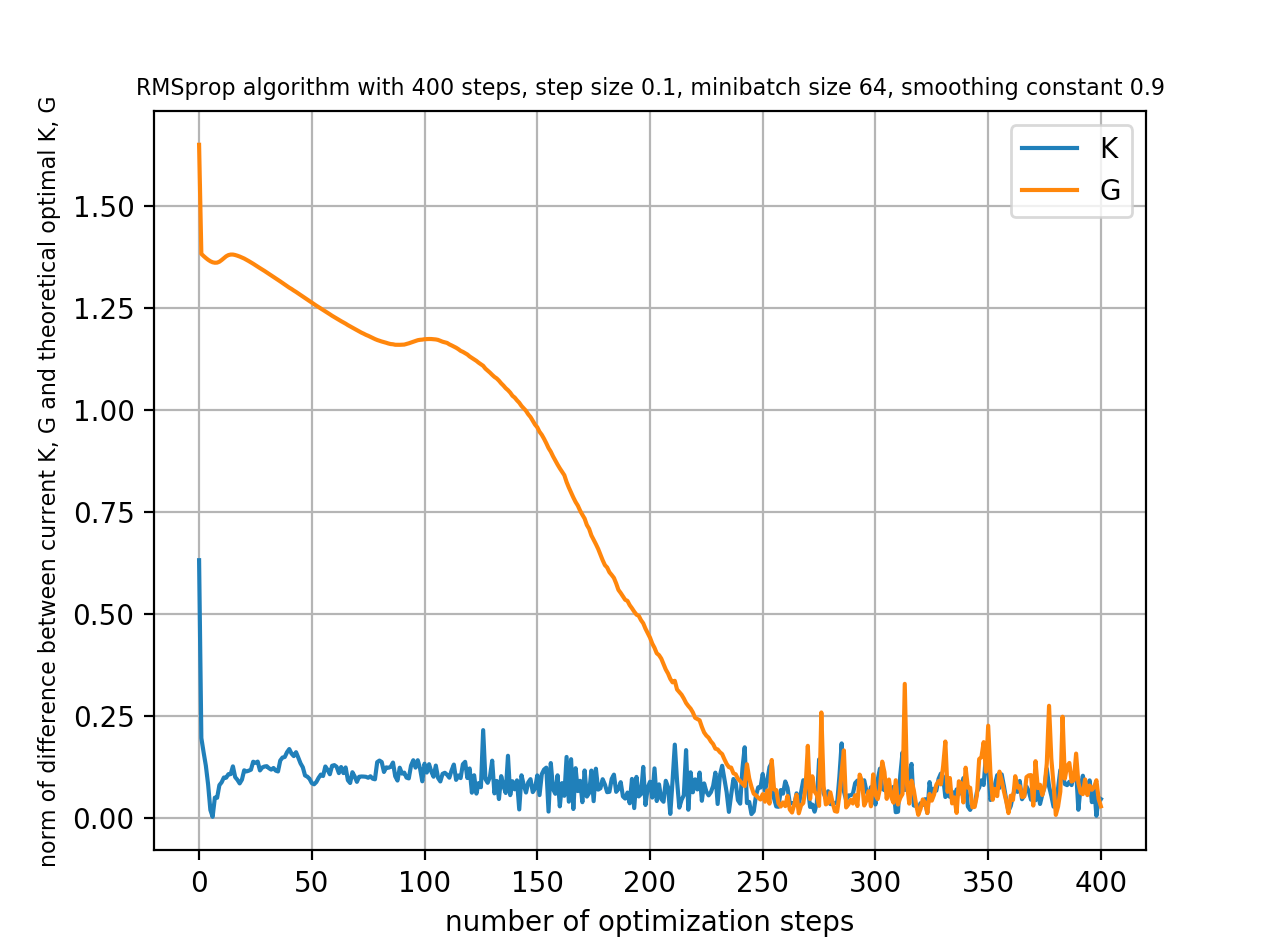
\includegraphics[width=1.0\textwidth]{Figures/d_M64.png}
		\caption{$M=64$: difference between $K$, $G$ and theoretical steady state $K$, $G$ w.r.t $n$}
	\end{minipage}%
	\begin{minipage}[t]{.28\paperwidth}
		\centering
		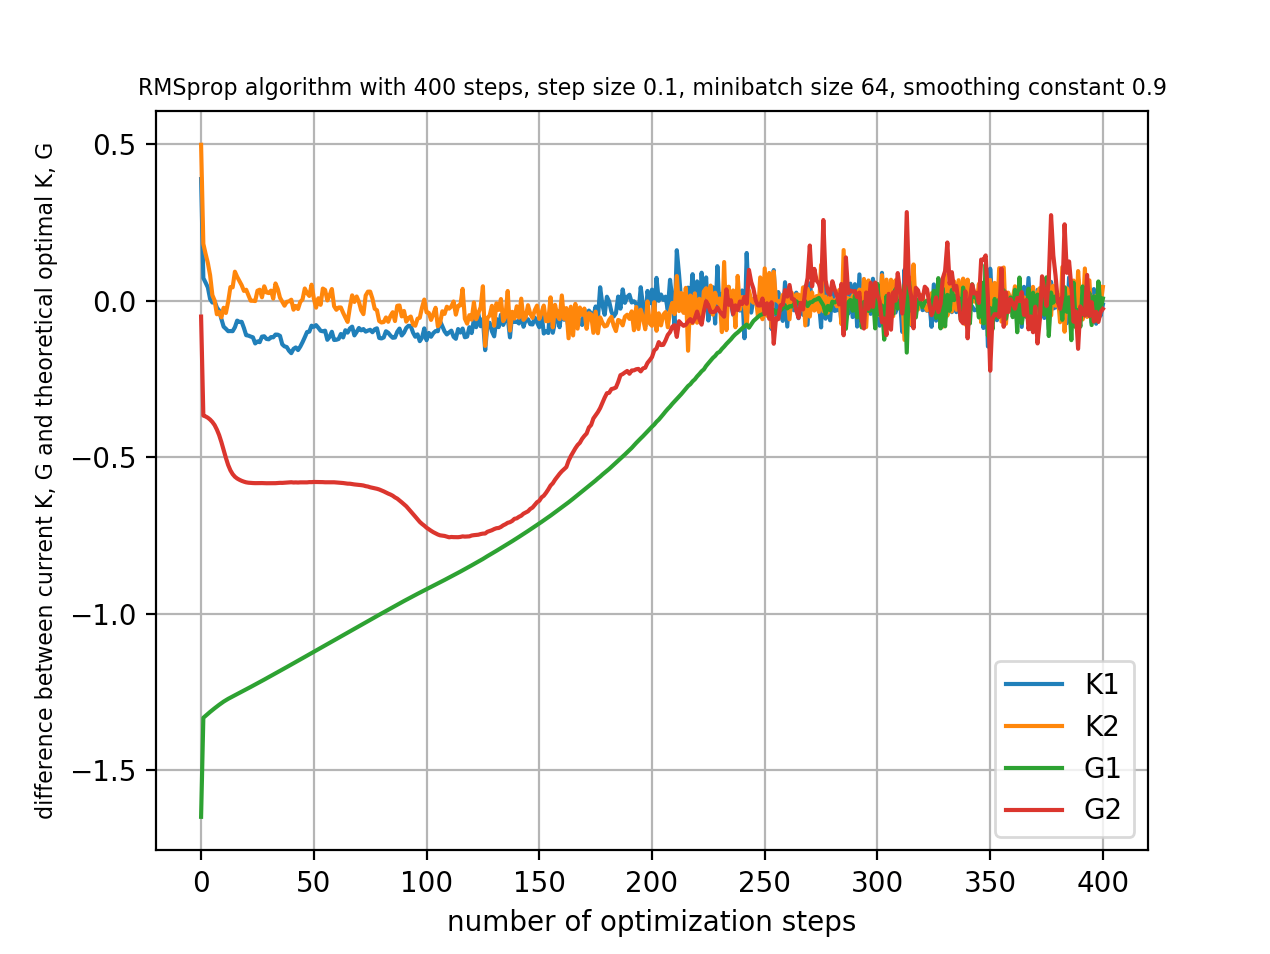
\includegraphics[width=1.0\textwidth]{Figures/d_M64_sep.png}
		\caption{$M=64$: difference between $K$, $G$ and theoretical steady state $K$, $G$ w.r.t $n$ (element-wise)}
	\end{minipage}
\end{figure}
\begin{figure}[h!]
	\centering
	\begin{minipage}[t]{.28\paperwidth}
		\centering
		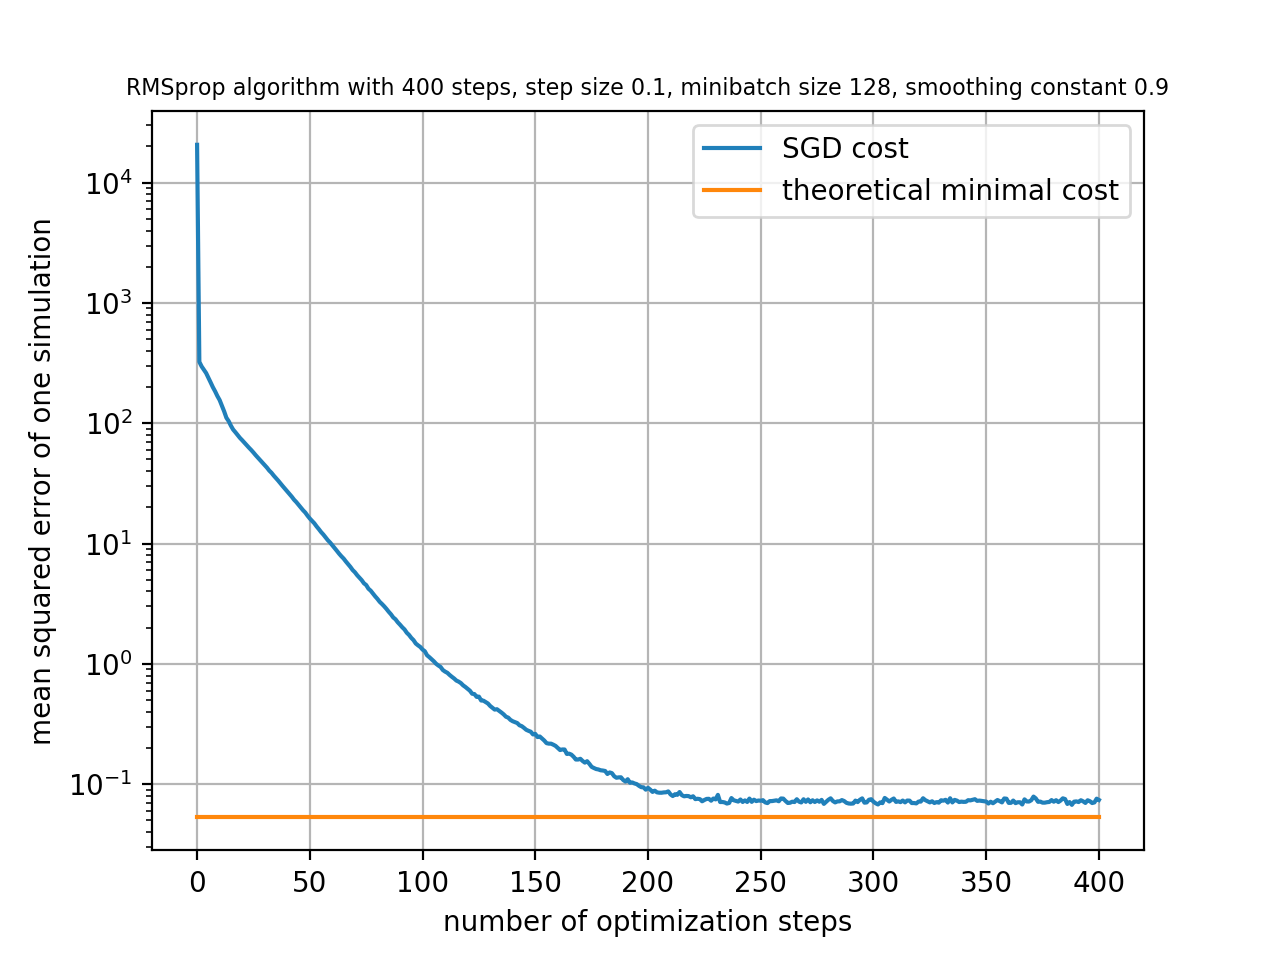
\includegraphics[width=1.0\textwidth]{Figures/M128.png}
		\caption{$M=128$: cost w.r.t $n$}
	\end{minipage}%
	\begin{minipage}[t]{.28\paperwidth}
		\centering
		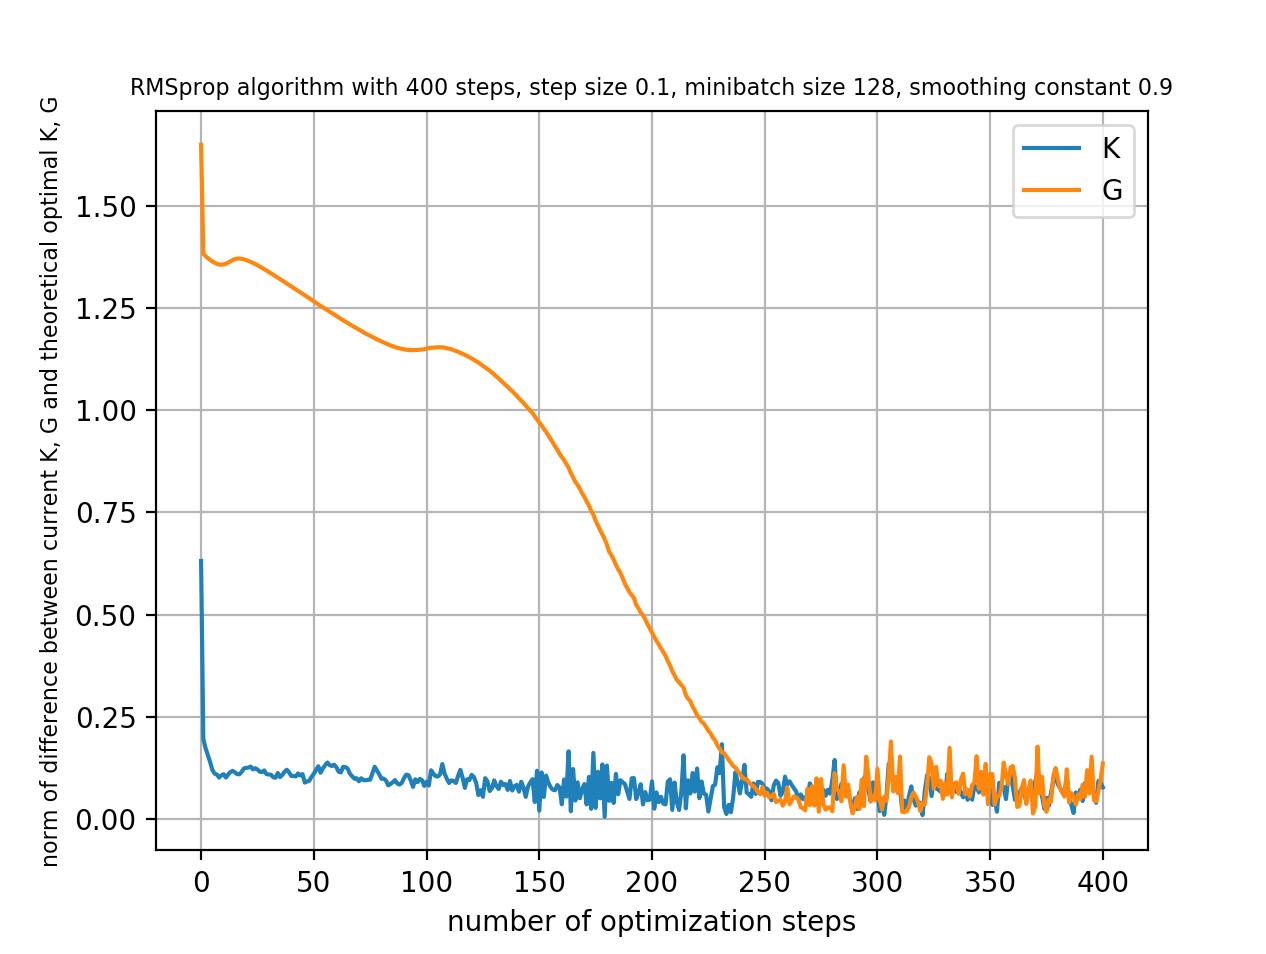
\includegraphics[width=1.0\textwidth]{Figures/d_M128.png}
		\caption{$M=128$: difference between $K$, $G$ and theoretical steady state $K$, $G$ w.r.t $n$}
	\end{minipage}%
	\begin{minipage}[t]{.28\paperwidth}
		\centering
		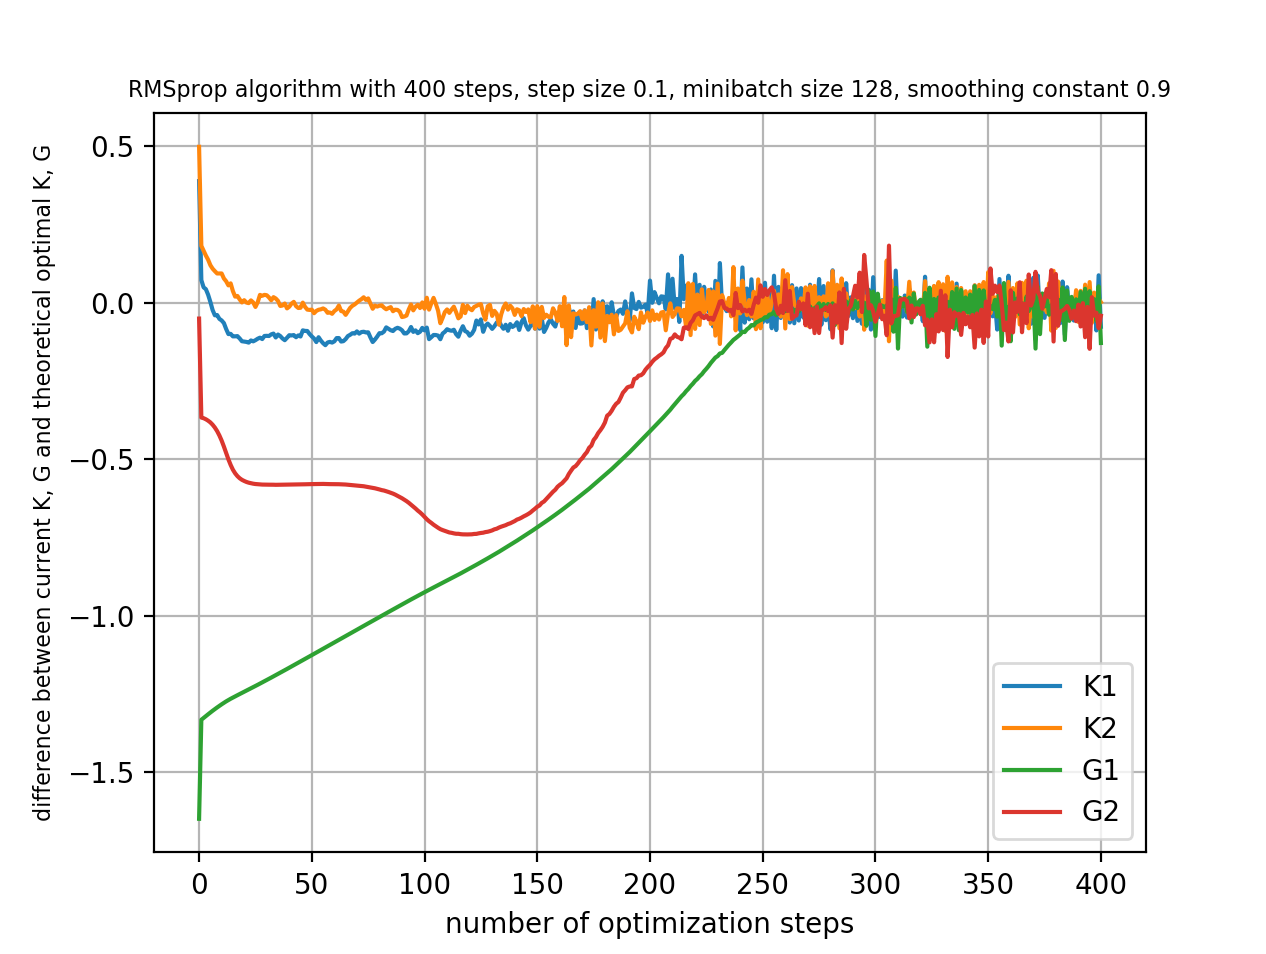
\includegraphics[width=1.0\textwidth]{Figures/d_M128_sep.png}
		\caption{$M=128$: difference between $K$, $G$ and theoretical steady state $K$, $G$ w.r.t $n$ (element-wise)}
	\end{minipage}
\end{figure}
\clearpage
\begin{figure}[h!]
	\centering
	\begin{minipage}[t]{.28\paperwidth}
		\centering
		\includegraphics[width=1.0\textwidth]{Figures/M256.png}
		\caption{$M=256$: cost w.r.t $n$}
	\end{minipage}%
	\begin{minipage}[t]{.28\paperwidth}
		\centering
		\includegraphics[width=1.0\textwidth]{Figures/d_M256.png}
		\caption{$M=256$: difference between $K$, $G$ and theoretical steady state $K$, $G$ w.r.t $n$}
	\end{minipage}%
	\begin{minipage}[t]{.28\paperwidth}
		\centering
		\includegraphics[width=1.0\textwidth]{Figures/d_M256_sep.png}
		\caption{$M=256$: difference between $K$, $G$ and theoretical steady state $K$, $G$ w.r.t $n$ (element-wise)}
	\end{minipage}
\end{figure}
\begin{figure}[h!]
	\centering
	\begin{minipage}[t]{.28\paperwidth}
		\centering
		\includegraphics[width=1.0\textwidth]{Figures/M512.png}
		\caption{$M=512$: cost w.r.t $n$}
	\end{minipage}%
	\begin{minipage}[t]{.28\paperwidth}
		\centering
		\includegraphics[width=1.0\textwidth]{Figures/d_M512.png}
		\caption{$M=512$: difference between $K$, $G$ and theoretical steady state $K$, $G$ w.r.t $n$}
	\end{minipage}%
	\begin{minipage}[t]{.28\paperwidth}
		\centering
		\includegraphics[width=1.0\textwidth]{Figures/d_M512_sep.png}
		\caption{$M=512$: difference between $K$, $G$ and theoretical steady state $K$, $G$ w.r.t $n$ (element-wise)\label{fig:d_M512_sep}}
	\end{minipage}
\end{figure}
\begin{figure}[h!]
	\centering
	\includegraphics[width=0.5\textwidth]{Figures/comp_M.png}
	\caption{Comparison of different $M$}
	\label{fig:comp_M}
\end{figure}
\clearpage

\paragraph{Experiments with Polyak averaging}
As mentioned in section 5.1, because of the presence of noise, instead of really converging to the optimum, it is more likely that after getting close to the optimum, the result of stochastic gradient descent oscillates around it. Inspired by the idea proposed in \cite{Polyak:1992:ASA:131092.131098}, instead of making the values of $K$ and $G$ at the last iteration as our final result, we keep track of the values of $K$, $G$ in the last $n_0$ iterations, and define the final $K$ as $\frac{1}{n_0}\sum_{i=n-n_0+1}^{n} K_i$, and the final $G$ as $\frac{1}{n_0}\sum_{i=n-n_0+1}^{n} G_i$, where $n_0$ is an additional hyper-parameter to choose. Intuitively, this can help reduce the effect of noise and make the final result closer to the optimum. Table \ref{table:3} compares the results of different $n$ and $n_0$ with $\beta = 0.9$, $\alpha = 0.1$, and $M = 8$. The first row in the table shows the theoretical result. We can see that by averaging, the difference between the ultimate $K$, $G$ from stochastic gradient descent and the theoretical solution is effectively narrowed. A closer look at the oscillation in last 200 iterations of gradient descent when $n$ is 400, 500, and 1000 is presented in figures \ref{fig:last200_n400} to \ref{fig:d_last200_n1000_sep}.\\
\begin{table}[h!]
	\begin{center}
		\begin{tabular}{|c|c|m{3.0cm}|m{3.0cm}|m{1.7cm}|m{1.7cm}|c|c|} 
			\hline
			$n$ & $n_0$ & ultimate $K$ & ultimate $G^T$ & final $K$ difference & final $G$ difference & final cost & testing cost \\ 
			\hline
			- & - & $\begin{bmatrix}1.12\times 10^{-1} \\ 2.44\times 10^{-3}\end{bmatrix}$ & $\begin{bmatrix}6.49\times 10^{-1} \\ -4.89\times 10^{-2}\end{bmatrix}$ & -- & -- & -- & $5.37\times 10^{-2}$\\
			\hline
			\hline
			400 & 1 & $\begin{bmatrix}1.13\times 10^{-1} \\ 1.91\times 10^{-2}\end{bmatrix}$ & $\begin{bmatrix}6.11\times 10^{-1} \\ -1.28\times 10^{-1}\end{bmatrix}$ & $1.67\times 10^{-2}$ & $8.81\times 10^{-2}$ & $7.45\times 10^{-2}$ & $7.01\times 10^{-2}$\\ 
			\hline
			400 & 10 & $\begin{bmatrix}1.08\times 10^{-1} \\ 1.65\times 10^{-2}\end{bmatrix}$ & $\begin{bmatrix}6.39\times 10^{-1} \\ -2.93\times 10^{-2}\end{bmatrix}$ & $1.47\times 10^{-2}$ & $2.18\times 10^{-2}$ & $7.63\times 10^{-2}$ & $7.03\times 10^{-2}$\\ 
			\hline
			400 & 100 & $\begin{bmatrix}1.05\times 10^{-1} \\ 8.66\times 10^{-3}\end{bmatrix}$ & $\begin{bmatrix}6.22\times 10^{-1} \\ -3.89\times 10^{-2}\end{bmatrix}$ & $9.17\times 10^{-3}$ & $2.83\times 10^{-2}$ & $7.64\times 10^{-2}$ & $7.03\times 10^{-2}$\\ 
			\hline
			500 & 1 & $\begin{bmatrix}1.35\times 10^{-1} \\ 1.40\times 10^{-2}\end{bmatrix}$ & $\begin{bmatrix}6.12\times 10^{-1} \\ -1.07\times 10^{-1}\end{bmatrix}$ & $2.59\times 10^{-2}$ & $6.87\times 10^{-2}$ & $5.86\times 10^{-2}$ & $7.12\times 10^{-2}$\\ 
			\hline
			500 & 100 & $\begin{bmatrix}1.06\times 10^{-1} \\ 8.00\times 10^{-3}\end{bmatrix}$ & $\begin{bmatrix}6.31\times 10^{-1} \\ -5.54\times 10^{-2}\end{bmatrix}$ & $7.80\times 10^{-3}$ & $1.87\times 10^{-2}$ & $5.71\times 10^{-2}$ & $7.05\times 10^{-2}$\\ 
			\hline
			1000 & 1 & $\begin{bmatrix}6.14\times 10^{-2} \\ 4.40\times 10^{-2}\end{bmatrix}$ & $\begin{bmatrix}6.00\times 10^{-1} \\ 4.85\times 10^{-2}\end{bmatrix}$ & $6.55\times 10^{-2}$ & $1.09\times 10^{-1}$ & $7.07\times 10^{-2}$ & $7.10\times 10^{-2}$\\ 
			\hline
			1000 & 200 & $\begin{bmatrix}1.06\times 10^{-1} \\ 3.45\times 10^{-3}\end{bmatrix}$ & $\begin{bmatrix}6.27\times 10^{-1} \\ -5.26\times 10^{-2}\end{bmatrix}$ & $6.50\times 10^{-3}$ & $2.16\times 10^{-2}$ & $6.93\times 10^{-2}$ & $7.00\times 10^{-2}$\\
			\hline
		\end{tabular}
	\end{center}
	\caption{Comparison of different $n$ and $n_0$}
	\label{table:3}
\end{table}
\begin{figure}[h!]
	\centering
	\begin{minipage}[t]{.28\paperwidth}
		\centering
		\includegraphics[width=1.0\textwidth]{Figures/last200_n400.png}
		\caption{$n = 400$: cost w.r.t $n$\label{fig:last200_n400}}
	\end{minipage}%
	\begin{minipage}[t]{.28\paperwidth}
		\centering
		\includegraphics[width=1.0\textwidth]{Figures/d_last200_n400.png}
		\caption{$n = 400$: difference between $K$, $G$ and theoretical steady state $K$, $G$ w.r.t $n$}
	\end{minipage}%
	\begin{minipage}[t]{.28\paperwidth}
		\centering
		\includegraphics[width=1.0\textwidth]{Figures/d_last_200_n400_sep.png}
		\caption{$n = 400$: difference between $K$, $G$ and theoretical steady state $K$, $G$ w.r.t $n$ (element-wise)}
	\end{minipage}
\end{figure}
\begin{figure}[h!]
	\centering
	\begin{minipage}[t]{.28\paperwidth}
		\centering
		\includegraphics[width=1.0\textwidth]{Figures/last200_n500.png}
		\caption{$n = 500$: cost w.r.t $n$}
	\end{minipage}%
	\begin{minipage}[t]{.28\paperwidth}
		\centering
		\includegraphics[width=1.0\textwidth]{Figures/d_last200_n500.png}
		\caption{$n = 500$: difference between $K$, $G$ and theoretical steady state $K$, $G$ w.r.t $n$}
	\end{minipage}%
	\begin{minipage}[t]{.28\paperwidth}
		\centering
		\includegraphics[width=1.0\textwidth]{Figures/d_last_200_n500_sep.png}
		\caption{$n = 500$: difference between $K$, $G$ and theoretical steady state $K$, $G$ w.r.t $n$ (element-wise)}
	\end{minipage}
\end{figure}
\begin{figure}[h!]
	\centering
	\begin{minipage}[t]{.28\paperwidth}
		\centering
		\includegraphics[width=1.0\textwidth]{Figures/last200_n1000.png}
		\caption{$n = 1000$: cost w.r.t $n$}
	\end{minipage}%
	\begin{minipage}[t]{.28\paperwidth}
		\centering
		\includegraphics[width=1.0\textwidth]{Figures/d_last200_n1000.png}
		\caption{$n = 1000$: difference between $K$, $G$ and theoretical steady state $K$, $G$ w.r.t $n$}
	\end{minipage}%
	\begin{minipage}[t]{.28\paperwidth}
		\centering
		\includegraphics[width=1.0\textwidth]{Figures/d_last_200_n1000_sep.png}
		\caption{$n = 1000$: difference between $K$, $G$ and theoretical steady state $K$, $G$ w.r.t $n$ (element-wise)\label{fig:d_last200_n1000_sep}}
	\end{minipage}
\end{figure}
\bibliographystyle{unsrt}
\bibliography{ref}
\end{document}